%
%================================================================%
%========================== AUTORES =============================%
% Eonay Barbosa Gurjão  email: eonay.web@gmail.com ==============%
% Klenilmar Lopes Dias  email: klenilmar@gmail.com ==============%
%================================================================% 
%================================================================%
%======================== Versão 2.3 ============================%
%================================================================%
\documentclass[12pt, % tamanho da fonte
	%openright,	% capítulos começam em pág ímpar
	oneside,		    % <twoside> para impressão em frente e verso
	a4paper,			% tamanho do papel
	english,			% Idioma adicional para hifenização
	brazil				% Idioma principal 
	]{abntex2}
	
%------------------------------------------------------------
%------------    Estrutura do texto   -----------------------         


\usepackage[small,bf]{caption} % captions e legends fonte reduzida

\usepackage{multirow} % Tabela mesclar linhas
\usepackage{multicol} % Tabela mesclar colunas

% Pacotes Básicos:
\usepackage{lmodern}			    % Usa a fonte Latin Modern			
\usepackage[T1]{fontenc}		  % Selecao de codigos de fonte.
\usepackage[utf8]{inputenc}		% Codificacao do documento (conversão automática dos acentos)
\usepackage{lastpage}			    % Usado pela Ficha catalográfica
\usepackage{indentfirst}		  % Indenta o primeiro parágrafo de cada seção.
\usepackage{color}				    % Controle das cores
\usepackage{graphicx}			    % Inclusão de gráficos
\usepackage{microtype} 		  	% para melhorias de justificação

% Pacotes Extras:

\usepackage{amsmath,amsthm}   %Símbolos Matemáticos
\usepackage{indentfirst} % Indenta primeiro parágrafo 
\usepackage[portuguese, ruled, linesnumbered,commentsnumbered, algo2e, vlined, lined, boxed, algochapter]{algorithm2e} % Algoritmos 
\usepackage{hyperref}
\usepackage[brazilian,hyperpageref]{backref}	 % Paginas com as citações na bibliograficas
\usepackage[alf]{abntex2cite}	% Citações padrão ABNT
\usepackage{etoolbox}
%\usepackage[num]{abntex2cite}  % Citações numéricas

%inclusao PDF
\usepackage{pdfpages}

% Defininfo Cores:
\definecolor{blue}{RGB}{25,25,112}

\makeatletter % informações do PDF
\hypersetup{ % pagebackref=true,
	pdftitle={\@title}, 
	pdfauthor={\@author},
    pdfsubject={\imprimirpreambulo},
	pdfcreator={LaTeX with abnTeX2},
	pdfkeywords={abnt}{latex}{abntex}{abntex2}{trabalho acadêmico}, 
	colorlinks=true,     % false: boxed links; true: colored links
    linkcolor=blue,          	% color of internal links
    citecolor=blue,        		% color of links to bibliography
    filecolor=magenta,      	% color of file links
    urlcolor=blue,
	bookmarksdepth=4 }
\makeatother
 

% -------------------------------------------- 
% Espaçamentos entre linhas e parágrafos 
\setlength{\parindent}{1.3cm} % O tamanho do parágrafo

% Controle do espaçamento entre um parágrafo e outro:
\setlength{\parskip}{0.2cm}  % tente também \onelineskip

% Definição de ambientes matemáticos em português 
\newtheorem{teorema}{Teorema}[chapter]
\newtheorem{axioma}{Axioma}[chapter]
\newtheorem{corolario}{Corolário}[chapter]
\newtheorem{lema}{Lema}[chapter]
\newtheorem{proposicao}{Proposição}[chapter]
\newtheorem{definicao}{Definição}[chapter]
\newtheorem{exemplo}{Exemplo}[chapter]
\newtheorem{observacao}{Observação}[chapter]

% Novos Comandos
\usepackage{tgtermes}
\renewcommand{\ABNTEXchapterfont}{\rmfamily\bfseries}

% Variáveis adicionais
\providecommand{\imprimirautorcite}{}
\newcommand{\autorcite}[1]{\renewcommand{\imprimirautorcite}{#1}} 
\providecommand{\imprimirsigla}{}
\newcommand{\sigla}[1]{\renewcommand{\imprimirsigla}{#1}}
\providecommand{\imprimiruf}{}
\newcommand{\uf}[1]{\renewcommand{\imprimiruf}{#1}}
\providecommand{\imprimircurso}{}
\newcommand{\curso}[1]{\renewcommand{\imprimircurso}{#1}}
\providecommand{\imprimirinstituto}{}
\newcommand{\instituto}[1]{\renewcommand{\imprimirinstituto}{#1}}
\providecommand{\imprimirdepartamento}{}
\newcommand{\departamento}[1]{\renewcommand{\imprimirdepartamento}{#1}}
\providecommand{\imprimirano}{}
\newcommand{\ano}[1]{\renewcommand{\imprimirano}{#1}}
\providecommand{\imprimirgrau}{}
\newcommand{\grau}[1]{\renewcommand{\imprimirgrau}{#1}}
\providecommand{\imprimirexaminadorum}{}
\newcommand{\examinadorum}[1]{
    \renewcommand{\imprimirexaminadorum}{#1}}
\providecommand{\imprimirexaminadordois}{}
\newcommand{\examinadordois}[1]{
    \renewcommand{\imprimirexaminadordois}{#1}}
\providecommand{\imprimirexaminadortres}{}
\newcommand{\examinadortres}[1]{
    \renewcommand{\imprimirexaminadortres}{#1}}
\providecommand{\imprimirexaminadorquatro}{}
\newcommand{\examinadorquatro}[1]{
    \renewcommand{\imprimirexaminadorquatro}{#1}}
\providecommand{\imprimirttorientador}{}
\newcommand{\ttorientador}[1]{
    \renewcommand{\imprimirttorientador}{#1}} 
\providecommand{\imprimirttcoorientador}{}
\newcommand{\ttcoorientador}[1]{
    \renewcommand{\imprimirttcoorientador}{#1}}
\providecommand{\imprimirttexaminadorum}{}
\newcommand{\ttexaminadorum}[1]{
    \renewcommand{\imprimirttexaminadorum}{#1}}
\providecommand{\imprimirttexaminadordois}{}
\newcommand{\ttexaminadordois}[1]{\renewcommand{
        \imprimirttexaminadordois}{#1}}
\providecommand{\imprimirttexaminadortres}{}
\newcommand{\ttexaminadortres}[1]{
    \renewcommand{\imprimirttexaminadortres}{#1}}
\providecommand{\imprimirttexaminadorquatro}{}
\newcommand{\ttexaminadorquatro}[1]{
    \renewcommand{\imprimirttexaminadorquatro}{#1}}

%----------------------------------------------------
\renewcommand{\imprimircapa}{  % Capa 
\begin{capa}

\hspace{-3cm}
\begin{tabular}{c c c}
    \centering
    
\includegraphics[scale=0.45]{figuras/profept_clean.jpg} &
    \large \imprimirinstituicao  &
    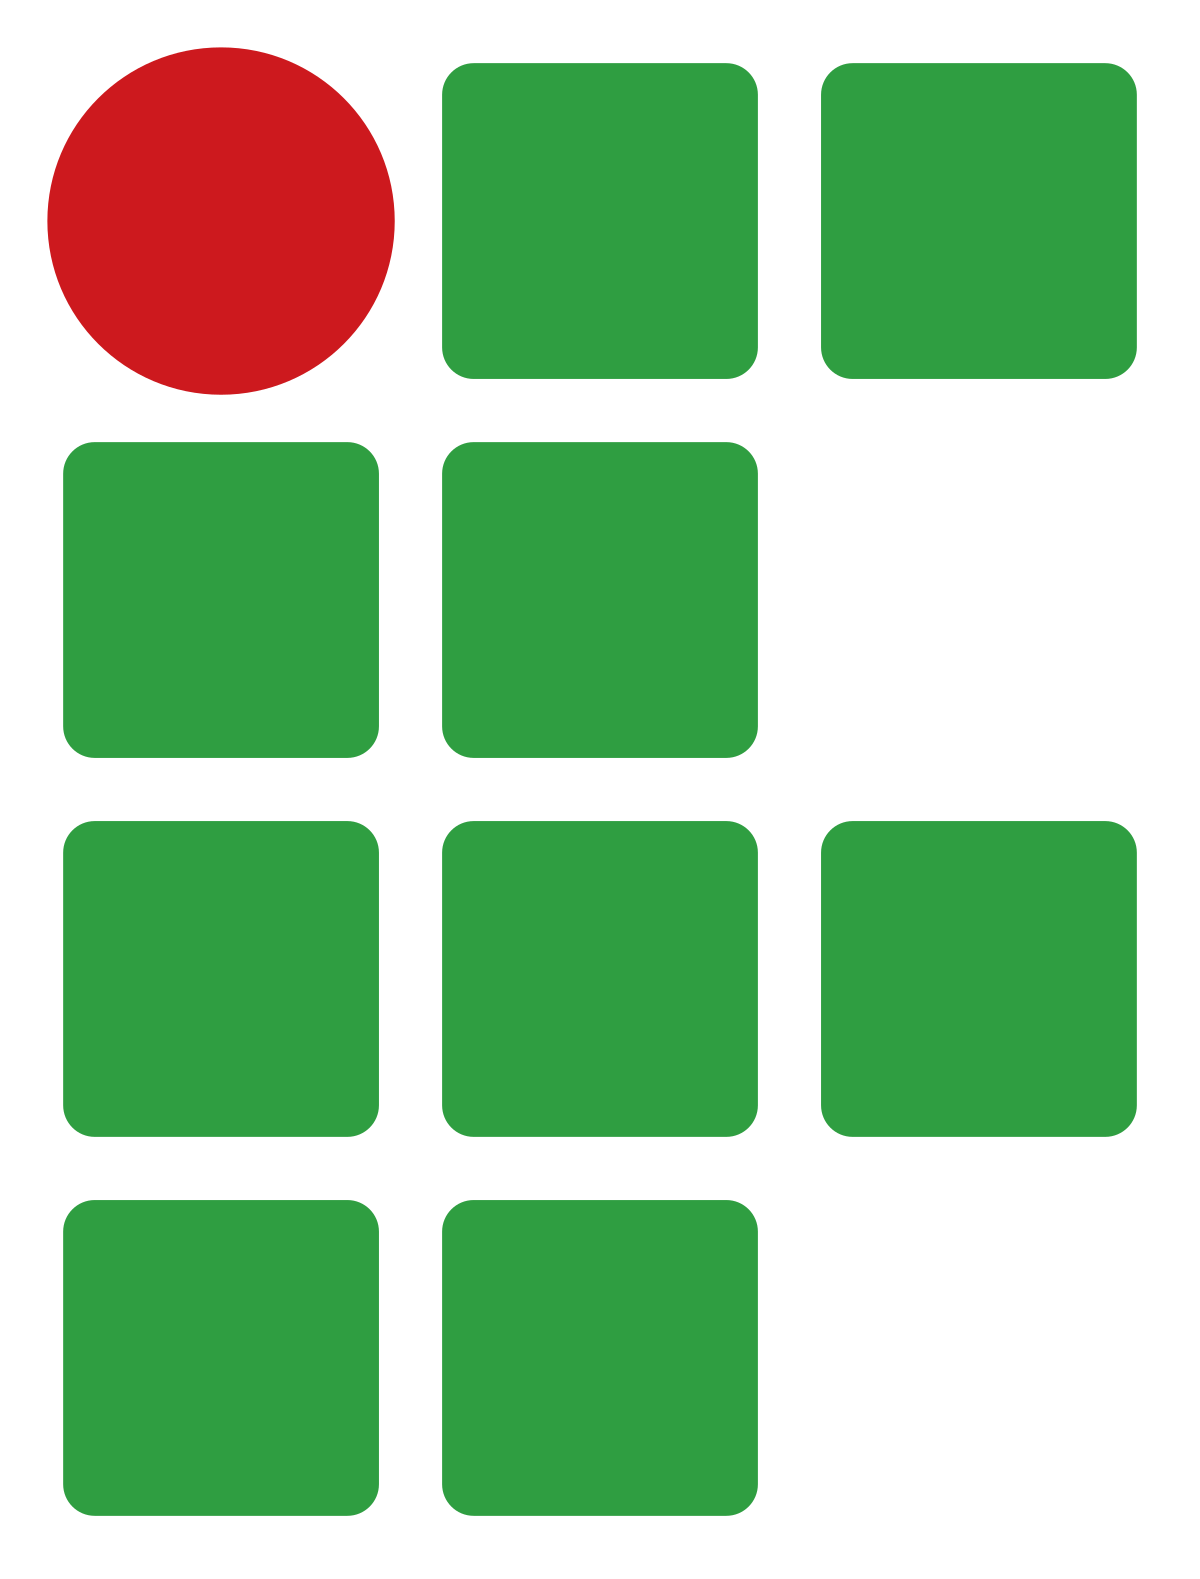
\includegraphics[scale=0.04]{figuras/ifap_clean.png}\\
    & \large \imprimirinstituto & \\
    & \large \imprimirdepartamento & \\
    
    
\end{tabular}






%\hspace{-1cm} \begin{minipage}[b]{0.19\linewidth}
%              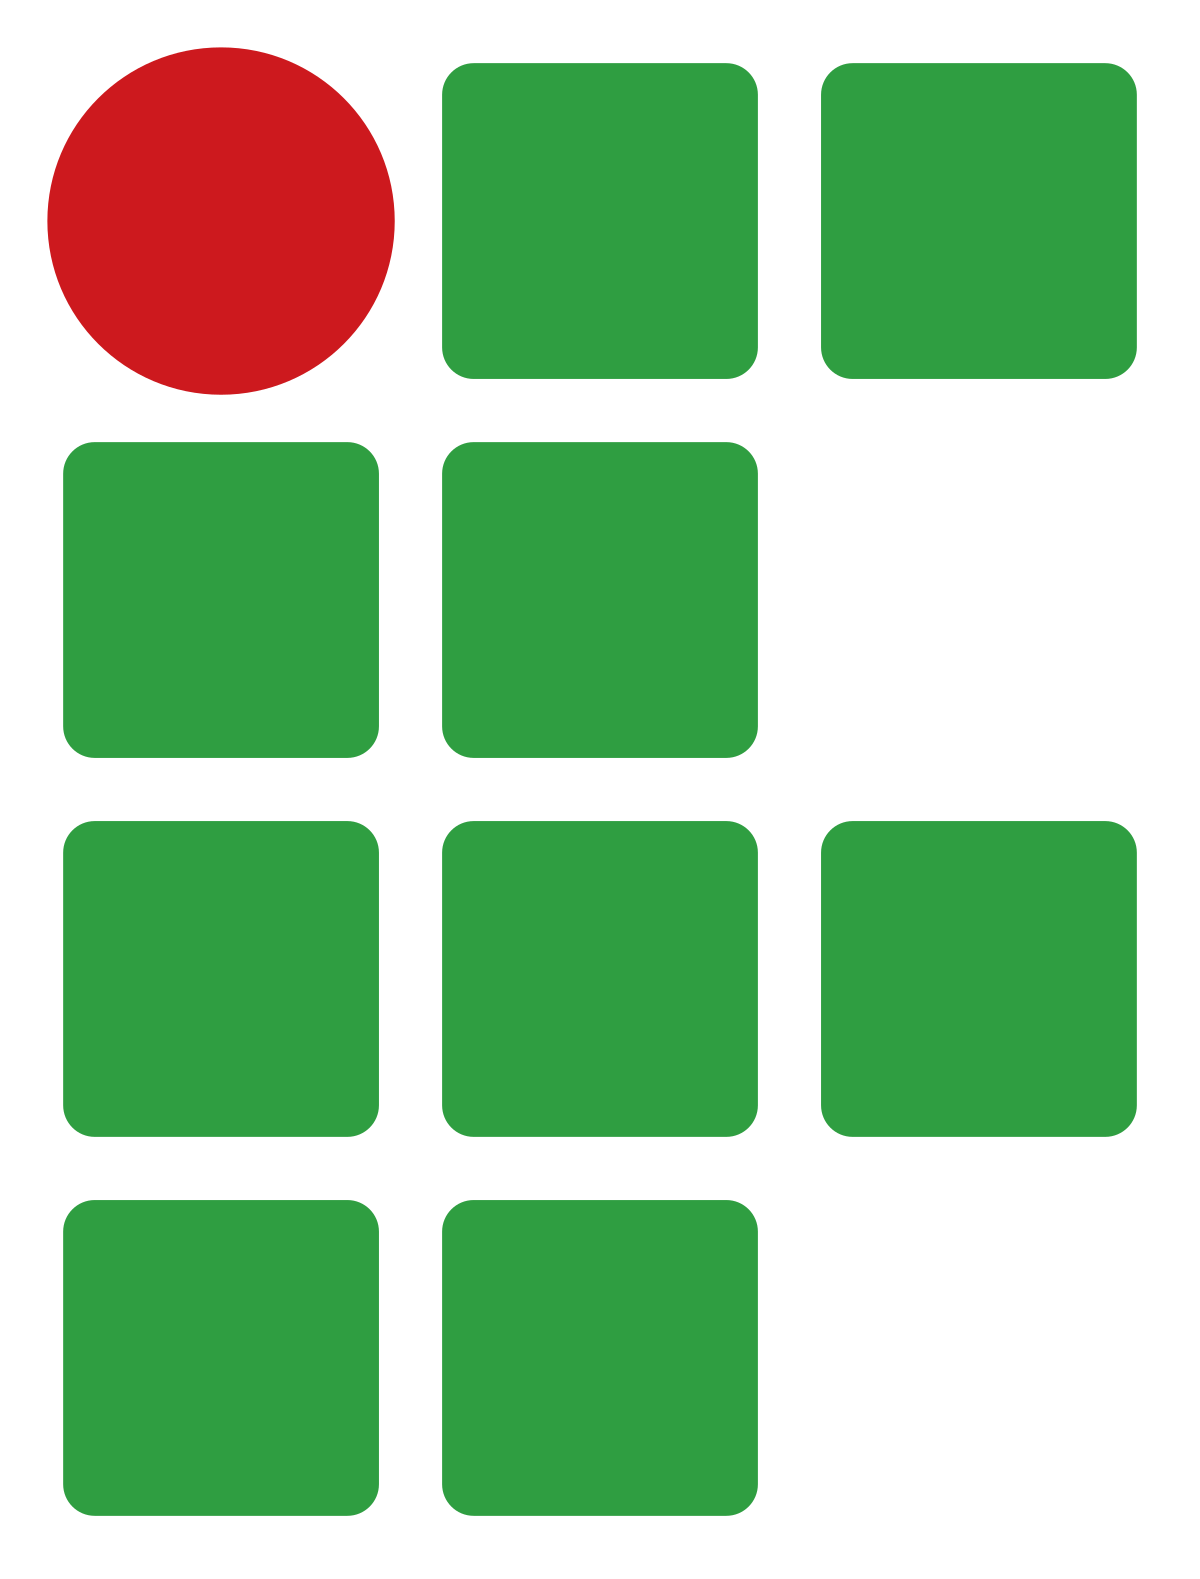
\includegraphics[scale=0.04]{figuras/ifap_clean.png}
%              \end{minipage}
%\hspace{-1cm} \begin{minipage}[b]{0.68\linewidth}
%              \begin{center}{\large
%              Ministério da Educação \\
%              \imprimirinstituicao \\
%              \imprimirinstituto \\
%              \imprimirdepartamento }\end{center}
%              \end{minipage} 
%\begin{minipage}[b]{0.15\linewidth}
%
\includegraphics[scale=0.45]{figuras/profept_clean.jpg}
%\end{minipage}


\vfill
        \begin{center}
        {\textsc{\huge \textbf{\imprimirtitulo}}}  \\
        
       
				\vspace{2cm}
				{\textsc {\large \imprimirautor}} 	
				\vfill
        {\large{\imprimirlocal~ - \imprimiruf \\ \imprimirano  }}
        \end{center}
\end{capa}   } % Capa

%----------------------------------------------------
\renewcommand{\imprimirfolhaderosto}{% folha de rosto
    \begin{center}
    {\textsc {\large \imprimirautor}}  \\
		\vfill
		{\textsc{\Huge \textbf{\imprimirtitulo}}}
    \end{center}
    \vfill 
    \begin{flushright} 
    \parbox{0.6\linewidth}{
		\imprimirtipotrabalho~ apresentada ao curso de \imprimircurso~ do \imprimirinstituicao~ como parte dos
		requisitos necessários para a obtenção do grau em \imprimirgrau. \\
		\vfill
		\textbf{\imprimirorientadorRotulo}~\imprimirorientador \\
		\vfill 
		\textbf{\imprimircoorientadorRotulo}~\imprimircoorientador}
   \end{flushright} 
   
	 \vfill
   \begin{center}
   {\large{\imprimirlocal~ - \imprimiruf \\ \imprimirdata}}
   \end{center} }  % folha de rosto

%----------------------------------------------------


  % Estrutura do Texto e Pacotes Principais

% -- Informações para Capa e Folha de Rosto: ---------------
\titulo{Práticas de ensino com matrizes}

% Ferramentas educacionais que auxiliam o ensino de Matrizes nos cursos de Licenciatura em Matemática no IFAP Campi Macapá


\autor{Eonay Barbosa Gurjão} \autorcite{Gurjão, Eonay Barbosa}
\local{Santana} \uf{AP}
\data{Dezembro de 2024} \ano{2024}
\orientador{Prof. Dr. Klenilmar Lopes Dias}  % Nome do orientador 
\ttorientador{Instituto Federal do Amapá - IFAP} % Instituição do orientador
%\coorientador{Prof. Dr. Nome do Coorientador} % Nome do coorientador
%\ttcoorientador{Universidade Federal de Ouro Preto} % Instituição do Coorientador
\instituicao{Instituto Federal do Amapá - Campus Santana} \sigla{IFAP}
\instituto{Pró-Reitoria de Extensão, Pesquisa e Inovação}
\departamento{Mestrado Profissional em Educação Profissional e Tecnológica}
\curso{Mestrado em Educação Profissional e Tecnológica}	
\tipotrabalho{Dissertação}
\grau{Mestre em Educação Profissional e Tecnológica}

%------Nomes dos examinadores.  
\examinadorum{Prof. Dr. Diego Armando Silva da Silva} \ttexaminadorum{Instituto Federal do Amapá - IFAP}
\examinadordois{Prof. Dr. Elivaldo Serrão Custódio} \ttexaminadordois{Universidade Federal do Amapá - UNIFAP}
%\examinadortres{Prof. Dr. Sérgio Orlando de Souza Batista} %\ttexaminadortres{Universidade Estadual do Amapá - UEAP}
%\examinadorquatro{Prof. Dr. Membro da Banca  4} \ttexaminadorquatro{Universidade Federal de ... - XXXX}

% ------------------------------------------------------
\makeindex   

\begin{document} % Início do documento

\frenchspacing  % Retira espaço obsoleto entre as frases.

% ----------------------------------------------------------
% -- Elementos Pré-Textuais: -------------------------------
\pagenumbering{roman}

\imprimircapa  % Capa
\imprimirfolhaderosto % Folha de rosto

% ---------------------------------------------------------------
% ----------------  Ficha Catalográfica  -------------------------
% ---------------------------------------------------------------
% Modelo de ficha catalográfica. Você deverá substituir esta
% folha na versão final da monografia por um pdf fornecido pela 
% biblioteca. Salve o modelo oficial como ficha_catalografica.pdf
% e use o comando abaixo para inseri-lo na versão final do texto.

%\begin{fichacatalografica}
%    \includepdf{ficha_catalografica.pdf}
%\end{fichacatalografica}



%% Modelo de Como fazer a Ficha Catalográfica:

\begin{fichacatalografica}
	\sffamily
	\vspace*{\fill}					% Posição vertical
	\begin{center}					% Minipage Centralizado
	\fbox{\begin{minipage}[c][8cm]{13.5cm}		% Largura
	\small
	\imprimirautorcite.
	%Sobrenome, Nome do autor
	
	\hspace{0.5cm}  \\
	\imprimirtitulo  / \imprimirautor. --, \imprimirano-
	
	\hspace{0.5cm} \pageref{LastPage} p. 1 :il. (colors; grafs; tabs).\\
	
	\hspace{0.5cm} \imprimirorientadorRotulo~\imprimirorientador\\
	
	\hspace{0.5cm}
	\parbox[t]{\textwidth}{\imprimirtipotrabalho~-~\imprimirinstituicao. ~\\
	\imprimirinstituto. \\ ~\imprimirdepartamento.}\\
	
	\hspace{0.5cm}
		1. EPT.
		2. Matrizes.
		3. Matemática.
        4. Ferramentas Educacionais.
        5. Construtivismo.			
	\end{minipage}}
	\end{center}
\end{fichacatalografica}



% ---------------------------------------------------------------
% ----------------  Folha de aprovação  -------------------------
% ---------------------------------------------------------------
% Modelo de Folha de aprovação. Você deverá substituir esta
% folha na versão final da monografia por um pdf fornecido pelo  
% colegiado do seu curso. Salve o modelo oficial como 
% folhadeaprovacao_final.pdf e use o comando abaixo para
% inseri-lo na versão final do texto.

%\begin{fichacatalografica}
%    \includepdf{folhadeaprovacao_final.pdf}
%\end{fichacatalografica} Esta folha será 


\begin{folhadeaprovacao}
\begin{center}
    {\large \textsc{\imprimirautor}} \\
   	\vspace{2cm}	
    {\textsc{\Large \textbf{\imprimirtitulo}}} \\
		\vspace{2cm}
\end{center}		


% defendida e aprovada em
\noindent \imprimirtipotrabalho~ apresentada em \imprimirlocal,~ \imprimirdata~,  pela banca examinadora constituída pelos professores:
\vspace{2cm}
\begin{center}

       \rule{10cm}{.1pt} \\
       {\imprimirorientador} \\
       {\imprimirttorientador} \\
			Orientador 
            \vfill
	   \ifdefvoid{\imprimircoorientador}{}{
       \rule{12cm}{.1pt} \\
       \imprimircoorientador \\
       \imprimirttcoorientador \\ 
           Coorientador 
	       \vfill}
       \rule{10cm}{.1pt} \\
       {\imprimirexaminadorum} \\ 
       {\imprimirttexaminadorum} \\
            Examinador Interno
            \vfill
        \ifdefvoid{\imprimirexaminadordois}{}{
        \rule{10cm}{.1pt} \\
        \imprimirexaminadordois \\
        \imprimirttexaminadordois \\
            Examinador Externo}
			\vfill
        \ifdefvoid{\imprimirexaminadortres}{}{
        \rule{10cm}{.1pt} \\
        \imprimirexaminadortres \\
        \imprimirttexaminadortres \\
            Examinador Externo}
			\vfill
        \ifdefvoid{\imprimirexaminadorquatro}{}{
        \rule{10cm}{.1pt} \\
        \imprimirexaminadorquatro \\
        \imprimirttexaminadorquatro \\
        Examinador Externo}
\end{center}
  
\end{folhadeaprovacao}
% --- 
\begin{dedicatoria}
   \vspace*{\fill}
   \centering
   \noindent
   \textit{Dedico este trabalho primeiramente a Deus, por ser essencial na minha vida em todos os momentos, ao meu pai Jose, minha mãe Ivanete e aos meus irmãos. A toda minha família que, com muito carinho e apoio, não mediram esforços para que eu chegasse até esta etapa de minha vida. Dedico também este trabalho aos meus avós paternos e maternos, ’In Memorian’, pela existência de meus pais, pois sem eles este trabalho e muitos dos sonhos não se realizariam.} 
	 \vspace*{\fill}
\end{dedicatoria}
\begin{agradecimentos}

Primeiramente, agradeço a Deus, por me guiar e fortalecer em cada passo desta jornada. Agradeço também à minha família, que me apoiou e incentivou, mesmo nos momentos mais desafiadores.

Em seguida, gostaria de expressar minha gratidão ao meu orientador, Professor Klenilmar Lopes Dias. Sua experiência, dedicação e constante incentivo foram fundamentais para o desenvolvimento deste trabalho. Sua orientação me proporcionou aprendizados valiosos.

Agradeço também meu colega Marcio Wendel de Lima Neri, que contribuíram significativamente para o aprimoramento desta pesquisa. Agradeço aos professores do ProfEPT, aos servidores do Campus Santana, em especial ao grupo de pesquisa GPTICAM, pelo indispensável apoio.

Aos professores envolvidos na pesquisa que, com sua participação ativa, possibilitaram a aplicação deste trabalho, favorecendo uma troca de conhecimentos riquíssima.

A todos que, de alguma forma, contribuíram para a realização deste trabalho, meu sincero agradecimento.

\end{agradecimentos}
\begin{epigrafe}
    \vspace*{\fill}
	\begin{flushright}
		\textit{"Há uma grande diferença entre saber o caminho e percorrer o caminho."\\
		        Matrix (1999).}
	\end{flushright}
\end{epigrafe}
%--------------------------------------------------------------------------
%--------------------- Resumo em Português --------------------------------
%--------------------------------------------------------------------------

\setlength{\absparsep}{18pt} % ajusta o espaçamento dos parágrafos do resumo
\begin{resumo}
O ensino mediado por elementos interativos em plataformas digitais tem como objetivo promover o engajamento dos estudantes e auxiliar na prática docente. Nesse contexto, a ferramenta \textbf{Mathix} foi desenvolvida para enfrentar as dificuldades recorrentes no ensino de matrizes, relacionadas à abstração matemática e à ausência de recursos interativos em métodos tradicionais. As tecnologias digitais educacionais têm demonstrado potencial para tornar o aprendizado mais dinâmico, acessível e alinhado às novas demandas tecnológicas, contribuindo para um ensino mais inclusivo. O \textbf{Mathix} oferece uma interface intuitiva e amigável, permitindo o uso de exercícios interativos e recursos visuais que auxiliam os docentes a explorar e manipular matrizes de forma prática e integrada ao aprendizado teórico. A metodologia de desenvolvimento incluiu uma revisão bibliográfica sobre o ensino de matrizes e o uso de tecnologias educacionais, além de entrevistas com professores para identificar as principais dificuldades enfrentadas no ensino desse tema. Após o desenvolvimento, o aplicativo foi submetido a testes com docentes, utilizando questionários para avaliar sua eficácia, interface e experiência do usuário antes e após o uso da ferramenta. O objetivo é consolidar o \textbf{Mathix} como um recurso inovador no ensino de matrizes, promovendo maior engajamento e aprendizado por meio da integração de práticas interativas e tecnológicas.


 \vspace{\onelineskip}
 \noindent
 \textbf{Palavras-chave}: EPT, Ferramentas Educacionais, Matrizes, Construtivismo, Matemática.
\end{resumo}

%--------------------------------------------------------------------------
%--------------------- Resumo em Inglês --------------------------------
%--------------------------------------------------------------------------
\begin{resumo}[Abstract]
 \begin{otherlanguage*}{english}
Teaching mediated by interactive elements on digital platforms aims to promote student engagement and assist teaching practice. In this context, the \textbf{Mathix} tool was developed to address the recurring difficulties in teaching matrices, related to mathematical abstraction and the lack of interactive resources in traditional methods. Digital educational technologies have shown potential to make learning more dynamic, accessible and aligned with new technological demands, contributing to more inclusive teaching. \textbf{Mathix} offers an intuitive and user-friendly interface, allowing the use of interactive exercises and visual resources that help teachers explore and manipulate matrices in a practical way that is integrated with theoretical learning. The development methodology included a literature review on the teaching of matrices and the use of educational technologies, as well as interviews with teachers to identify the main difficulties faced in teaching this subject. After development, the application was tested with teachers, using questionnaires to evaluate its effectiveness, interface and user experience before and after using the tool. The aim is to consolidate \textbf{Mathix} as an innovative resource for teaching matrices, promoting greater engagement and learning through the integration of interactive and technological practices.


   \vspace{\onelineskip}
   \noindent 
   \textbf{Keywords}: EFA, Educational Tools, Matrices, Constructivism, Mathematics.
 \end{otherlanguage*}
\end{resumo}

\renewcommand{\listfigurename}{Lista de figuras}
\pdfbookmark[0]{\listfigurename}{lof}
\listoffigures*   % Cria a Lista de Figuras
\cleardoublepage

\pdfbookmark[0]{\listtablename}{lot}
\listoftables*  % Cria a lista de Tabelas
\cleardoublepage

%\renewcommand{\listalgorithmcfname}{Lista de algoritmos}
%\pdfbookmark[0]{\listalgorithmcfname}{lof}
%\listofalgorithmes   % Cria a lista de Tabelas
%\cleardoublepage

% ---------------------------------------------------
% ------ Lista de abreviaturas e siglas -------------
% ---------------------------------------------------
\begin{siglas}
\item[ABNT] Associação Brasileira de Normas Técnicas
\item[IFAP] Instituto Federal do Amapá
\item[IHC] Interação Humano-Computador
\item[BNCC] Base Nacional Comum Curricular
\item[PE] Produto Educacional
\item[UI] Interface do Usuário
\item[UX] Experiência do Usuário
\item[EPT] Educação Profissional e Tecnológica
\item[TDIC] Tecnologia Digitais da Informação e Comunicação 
\item[TIC] Tecnologias de Informação e Comunicação
\item[CEFET] Centros Federais de Educação Tecnológica
\item[UTFPR] Universidade Tecnológica Federal do Paraná
\item[CONIF] Conselho Nacional dos Institutos Federais
\item[LDB]  Lei de Diretrizes e Bases da Educação Nacional
\item[CONSUP] Conselho Superior 
\item[TCLE] Termo de Esclarecimento Livre Esclarecido 
\item[CEP] Comitê de Ética em Pesquisa 
\item[CONEP] Comissão Nacional de Ética em Pesquisa 
\item[CNS] Conselho Nacional de Saúde 
\item[PMV] Produto Mínimo Viável 
\item[REA] Recurso Educacional Aberto 
\item[NIT] Núcleo de Inovação Tecnológica 
\item[PPC] Plano Pedagógico de Curso
\item[SBM] Sociedade Brasileira de Matemática
\item[SBMAC] Sociedade Brasileira de Matemática Aplicada e Computacional 
\item[PWA] Aplicações Web Progressivas
\item[GPTICAM] Grupo de Pesquisa em Tecnologias da Informação e Comunicação na Amazônia 
\item[AVA] Ambiente Virtual de Aprendizagem 
\item[EAD] Educação a Distância 
\item[CNMAC] Congresso Nacional de Matemática Aplicada e Computacional 
\item[SENACEM] Seminário Nacional do Ensino Médio 
\end{siglas}
%% ---------------------------------------------------
% ----------- Lista de símbolos ---------------------
% ---------------------------------------------------

\begin{simbolos}
  \item[$ \Gamma $] Letra grega Gama
  \item[$ \Lambda $] Lambda
  \item[$ \zeta $] Letra grega minúscula zeta
  \item[$ \in $] Pertence
\end{simbolos}


\pdfbookmark[0]{\contentsname}{toc}
\tableofcontents*
\cleardoublepage




% ----------------------------------------------------------
% -- Capítulos do Trabalho: --------------------------------
\pagenumbering{arabic} \setcounter{page}{1}
\textual 
\chapter{Introdução}
\label{introducao}


No cenário atual da educação, a incorporação de tecnologias inovadoras é fundamental para aprimorar as práticas docentes e enriquecer a experiência de aprendizado. Nesse contexto, este trabalho apresenta o desenvolvimento de um software específico para auxiliar no ensino da matemática, com foco no ensino profissional e tecnológico, especialmente na introdução ao conteúdo de matrizes. O produto educacional foi projetado para aumentar a eficácia no aprendizado dos estudantes, simplificando conceitos complexos. Além disso, serve como uma ferramenta de apoio para que os educadores explorem e ampliem suas abordagens pedagógicas.

Por meio de uma interface intuitiva e recursos interativos, o software busca oferecer uma nova perspectiva para o ensino e a compreensão do conteúdo de matrizes, em ambientes acadêmicos formais e informais. Desde o ensino de conceitos fundamentais até a aplicação em contextos de exercícios, cada aspecto do software foi meticulosamente projetado para promover a compreensão profunda conceitual dos princípios matemáticos do uso de matrizes.

A ferramenta oferece uma ampla variedade de exercícios automatizados e dinâmicos, permitindo que os educadores personalizem as atividades de acordo com as necessidades específicas de suas turmas e currículos. Dessa forma, não só se fortalece o aprendizado individualizado, como também se fomenta um ambiente de sala de aula invertida que estimula e proporciona uma descoberta entre alunos e professores.

Com a adoção do software no ensino da matemática, os educadores terão acesso a uma ferramenta poderosa que simplifica a preparação de aulas e potencializa o impacto no desenvolvimento dos alunos, promovendo um aprendizado mais atrativo e interativo.





%Uma abordagem de aprendizagem ativa é uma técnica de ensino baseada em atividades que permite aos alunos participar e, de fato, tornar-se protagonistas no processo de construção de seu próprio conhecimento. Ou seja, são abordagens baseadas menos na transferência de informações e mais no desenvolvimento de habilidades.


%Segundo \citeonline{wenglinsky2005using}, a tecnologia educacional não deve ser observada como um fenômeno isolado, mas deve sim ser considerada uma peça do quebra-cabeça de como os professores ensinam e os alunos aprendem. Assim, muitos pesquisadores educacionais indicam que a integração de tecnologia na sala de aula pode ser vantajosa para alunos e professores. Por exemplo, a tecnologia pode auxiliar a motivar os alunos e proporcionar-lhes habilidades importantes para reforçar seu aprendizado \cite{silva2021integraccao}.



%Dentre as metodologias ativas mais comuns, podemos citar a aprendizagem baseada em problemas, a aprendizagem baseada em equipes, a aprendizagem baseada em projetos, a aprendizagem baseada em letramento informacional, a instrução por colegas e a gamificação. Entretanto, todas elas têm o mesmo fundamento na problematização e visam a aprendizagem significativa \cite{moreira2016accoes}.



%Um diagnóstico inicial focou no plano de curso de Licenciatura em Matemática em face da análise dos documentos públicos do curso, onde algumas características foram levantadas, como os documentos de criação e autorização de curso, informações dos currículos dos docentes, documentos públicos da coordenação e plano pedagógico com os instrumentos ementários assim como os próprios conteúdos.

%No estudo preliminar em análise do plano de curso apenas uma única ferramenta educacional é citada, o MatLab e, com intuito de aprofundar na investigação, partiu-se para procura dos planos de aula, ou seja, o planejamento em detalhes da prática docente onde foi identificado que o mesmo não encontra-se disponível à publico encontra-se é de caráter público assim impossibilitando uma análise completa para afirmar ou aferir o fato, apenas algumas poucas evidências.

%\url{http://www.uel.br/projetos/matessencial/basico/medio/matrizes.html#menu}


%O projeto de pesquisa é na área de educação na subárea de ensino com a temática de ferramentas educacionais aplicadas no currículo do curso e voltado para a componente de matrizes no curso de Licenciatura em Matemática do Instituto Federal do Amapá (IFAP) no Câmpus Macapá na perspectiva docente para adoção nas aulas.


%Busca-se auxiliar na aplicação de Metodologias Ativas com Gameficação no ensino da Matemática. Desenvolver uma aplicação sobre uma plataforma web para utilização na prática do ensino de matrizes e aplicar técnica de Inteligência Artificial com foco em aprendizagem por reforço para uma aprendizagem significativa mediadas por tecnologia digitais da informação e comunicação (TDIC).

%A proposta de pesquisa busca identificar, propor e aplicar metodologias inovativas e tecnológicas na prática docente para uso de ferramentas no ensino, buscando alternativas para as práticas tradicionais na Educação Profissional e Tecnológica (EPT). Nessa concepção de EPT, o ambiente virtual e as novas tecnologias são utilizados para disponibilizar diferentes possibilidades de aprendizagens, para se adaptar às mudanças e atender ao "novo estudante" da era digital, que participa ativamente da construção do conhecimento e frente a isso, o docente deverá rever sua prática pedagógica.


\section{Problemática}

Quais são as características de ferramentas educacionais eficazes para o ensino presencial do conteúdo de matrizes nos cursos de Licenciatura em Matemática?



\section{Hipóteses}
\label{sec:hipoteses}

\begin{itemize}
    \item A aplicação de ferramentas educacionais promove maior engajamento em sala de aula no ensino de matrizes;
    \item Recursos visuais interativos podem melhorar a compreensão do conteúdo e dinamizar a prática docente no ensino de matrizes;
    \item O uso de ferramentas tecnológicas em ambientes virtuais de aprendizagem contribui significativamente para o ensino e a aprendizagem de matrizes;
\end{itemize}



\section{Objetivos}
\label{objetivos}

%O objetivo geral é analisar as ferramentas aplicadas pelos docentes no ensino de matrizes. Os objetivos específico do projeto segue:

O objetivo geral é identificar metodologias inovativas e tecnológicas aplicadas pelos docentes no currículo do curso e voltado para ao componente de matrizes no curso de Licenciatura em Matemática do Instituto Federal do Amapá (IFAP) no Campus Macapá. Os objetivos específico do projeto segue:

\begin{itemize}
    \item Identificar ferramentas educacionais utilizadas no ensino de matrizes na Licenciatura em Matemática do IFAP - Campus Macapá;

    \item Classificar os recursos utilizados para o ensino de matrizes, com foco em metodologias inovadoras e tecnológicas;

    \item Propor uma aplicação baseada em plataforma web com gamificação para o ensino de matrizes;
    
    \item Avaliar o impacto de ferramentas tecnológicas aplicadas ao ensino de matrizes;
    
    \item Propor um modelo de relatório acadêmico em formato LaTeX para o ProfEPT, simplificando a aplicação das normas ABNT, abstraindo suas complexidades.
\end{itemize}




            
\section{Justificativa}
\label{sec:justificativa}

Conteúdo de matrizes é aplicado em diversas disciplinas e cursos, abordado sob diferentes perspectiva e de diferentes aspectos incluindo a aplicação como estrutura de dados, assim tem o potencial de ser trabalhado de forma transdisciplinar. A matriz se aplica em diversas áreas de conhecimento sendo de ciências exatas ou não, onde pode-se aplicar a aprendizagem significativa com outras técnicas em sala e metodologias ativas e criativas dentre outras.

\citeonline{levy1999cibercultura} argumenta que as novas tecnologias devem ser empregadas para enriquecer o ambiente educacional. Para dar conta dessa inserção no cenário educacional é solicitado aos professores novos saberes e competências para lidar criticamente com as Tecnologias de Informação e Comunicação (TIC) em seu dia a dia docente.

Na mesma perspectiva \citeonline{kenski2001direccao} assegura ser necessário ao docente conhecer o computador, os suportes midiáticos e todas as possibilidades educacionais e interativas para aproveitá-las nos suportes midiáticos nas mais variadas situações de ensino-aprendizagem e nas mais diferentes realidades educacionais. O professor passa a ser o encarregado de uma grande responsabilidade de utilizar as TIC como recurso para construir e difundir conhecimentos em sua prática docente.

O uso de ferramentas tecnológicas na educação profissional potencializa o ensino, especialmente para alunos já familiarizados com essas tecnologias, papel docente é mediar o conhecimento aplicando diversos recursos, assim expandido as ações de reflexão e autonomia dos alunos. A prática docente deve adaptar a diferentes possibilidades, formas e formatos e, neste contexto a proposta é voltada a prática inovativa docente adotando elementos para intermediar o ensino.

A proposta tem potencialidade de trabalhar com aprendizagem combinada a sala de aula invertida (\textit{Blended Learning e Flipped Classroom}) podendo ser aplicado para dentro e fora da sala de aula, ou seja, nos espaços tradicionais formais e não formais. Assim podendo viabilizar também de forma a dar autonomia aos estudantes, colocando-os no centro do processo como protagonista das ações, estimulando a pensar e resolver problemas de forma independente.

As metodologias de \textit{blended learning} (no formato híbrido) e \textit{flipped classroom} (ensino invertido) formam perfis de profissionais mais engajados e menos dependentes ou autodidatas para certas atividades, resultando em uma aprendizagem personalizada e efetiva. Restando ao professor a tarefa trivial de mediar o uso e o planejamento dos objetivos de aprendizagem.




















\section{Trabalhos Relacionados}
\label{trabalhos_relacionados}

No trabalho de \citeonline{florencio2021perspectivas} é proposto o uso de uma ferramenta digital (Jamboard) para mediação em aulas remotas na perspectiva docente de caráter qualitativo, aplicado em um estudo de caso. A experiência trouxe mecanismos para vivenciar o ensino remoto utilizando ferramentas tecnológicas por meio de metodologias ativas, ressaltando comparações entre o ensino presencial e o remoto \cite{florencio2021perspectivas}.

Diferentemente do trabalho supracitado a proposta é investigar a prática docente com o uso de ferramentas tecnológicas no ensino presencial e híbrido, com intervenção para avaliar a proposta em conjunto com a componente de matrizes. Assim para uso de novos recursos que favorecem   a   ampliação   das   técnicas   didáticas   pelos   educadores.

Corroborando com a proposta de pesquisa no trabalho de \citeonline{ferramenta_padlet} foca na ferramenta digital Padlet como recurso visual e alternativo para organização de conteúdos para as apresentações de seminários avaliativos como metodologia ativa que promove autonomia e a interação.

Correlacionado com trabalho supracitado, o o uso de matrizes como recurso visual em plataformas web, promovendo autonomia e integração com o conteúdo e de apoio ao docente como recurso educacional aberto. As características do Produto Educacional (PE) abstraem características dos projetos retratados nesta relatório.









\section{Organização do Texto}
\label{organizacao_texto}

Este trabalho está organizado da seguinte forma: inicialmente no Capitulo \ref{introducao} uma breve introdução, seguida do referencial teórico, que apresenta a fundamentação histórica da educação profissional e tecnológica, as tecnologias digitais da informação e comunicação aplicadas a prática docente e a BNCC no Capítulo \ref{fundamentacao}. No Capítulo \ref{metodologia} com percurso metodológico e métodos utilizados. Os resultados e discussões serão tratados no  Capítulo \ref{resultados} e, por fim as considerações finais e limitações no Capítulo \ref{conclusao}.


\chapter{Fundamentação}
\label{fundamentacao}


\section{Bases da Educação Profissional e Tecnológica}
\label{ept}

As instituições que compõem atualmente a Rede Federal de Educação Profissional, Científica e Tecnológica têm origem, em sua maioria, nas 19 escolas de aprendizes artífices criadas por decreto presidencial em 1909, durante o governo de Nilo Peçanha. \cite{silva2009institutos}. Originalmente subordinadas ao Ministério dos Negócios da Agricultura, Indústria e Comércio, essas escolas passaram, em 1930, a ser supervisionadas pelo recém-criado Ministério da Educação e Saúde Pública.


Em janeiro de 1937, a Lei nº 378 extinguiu as escolas de aprendizes artífices, substituindo-as pelos liceus industriais \cite{candido2019era}. Um ano após o ensino profissional ser considerado de nível médio, em 1942, os liceus passam a se chamar escolas industriais e técnicas, e, em 1959, escolas técnicas federais, configuradas como autarquias.

Ao longo desse mesmo tempo vai se constituindo uma rede de escolas agrícolas – Escolas Agrotécnicas Federais, com base no modelo escola fazenda e vinculadas ao Ministério da Agricultura \cite{silva2009institutos}. Em 1967, essas escolas fazendas passam para o então Ministério da Educação e Cultura tornando-se escolas agrícolas. Em 1978, três escolas federais, do Rio de Janeiro, Minas Gerais e Paraná são transformadas em Centros Federais de Educação Tecnológica (CEFET) equiparando-se, no âmbito da educação superior, aos centros universitários \cite{silva2009institutos}.

Em 29 de dezembro de 2008, a publicação da Lei 11.892, que no âmbito do Ministério da Educação criou os Institutos Federais de Educação, Ciência e Tecnologia, os quais apresentam um novo modelo de Educação Profissional, estruturados a partir dos CEFETs, escolas técnicas e agrotécnicas federais e escolas vinculadas às universidades federais \cite{garcia2018educaccao}.


Em 2019, já são mais de 661 unidades sendo estas vinculadas a 38 Institutos Federais, 02 Centros Federais de Educação Tecnológica (Cefet), a Universidade Tecnológica Federal do Paraná (UTFPR), a 22 escolas técnicas vinculadas às universidades federais e ao Colégio Pedro II \cite{conif2023}. 

Neste contexto, a Educação Profissional e Tecnológica (EPT) busca não apenas oferecer conhecimentos técnicos específicos, mas também desenvolver habilidades socioemocionais e competências transversais. A interdisciplinaridade torna-se essencial, permitindo aos estudantes uma formação mais abrangente e adaptável às constantes mudanças nas dinâmicas
profissionais. A EPT se sustenta em um tripé: Trabalho como princípio educativo; Politecnia e Formação humana integral, Figura \ref{fig:bases_ept}.

\begin{figure}[h!]
    \centering
    \caption{Bases Conceituais da EPT}
    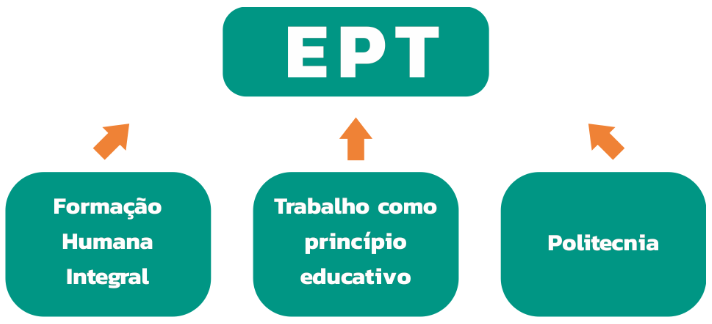
\includegraphics[scale=0.4]{figuras/bases_ept_v.png}
    \legend{Fonte: \citeonline{sousa2019guia}}
    \label{fig:bases_ept}
\end{figure}




\subsection{Trabalho Como Princípio Educativo}
\label{trab_prin_edu}

O trabalho é um processo central para a formação e a realização humanas, representando a interação com o mundo natural para a satisfação de necessidades básicas e complexas.

De acordo com \citeonline{frigotto2009teoria} , é por meio do trabalho que o ser humano transforma a natureza, atendendo tanto às suas necessidades básicas quanto às mais complexas, como culturais, lúdicas, estéticas e afetivas. \citeonline{de2018trabalho} destacam que o ser humano produz sua realidade e dela se apropria, motivo pelo qual o trabalho é um princípio educativo.


O trabalho como princípio educativo orienta a formação para a emancipação humana, para o desenvolvimento autônomo do ser rumo à expressão de suas potencialidades para transformação da realidade social coletiva. \citeonline{kulesza2019trabalho} registra que o trabalho como princípio educativo se relaciona com uma postura ativa e criativa perante o mundo.








\subsection{Politecnia}
\label{politecnia}

Derivado do trabalho como princípio educativo, o conceito de politecnia, segundo \citeonline{maciel2017fundamentos}, remonta às três dimensões da educação propostas por Karl Marx: educação intelectual, física e tecnológica - este último termo foi posteriormente modificado para educação politécnica.

O conceito de politecnia está relacionado à ideia de que a formação dos indivíduos deve abranger uma diversidade de conhecimentos e habilidades que vão além de uma única especialização técnica. Conforme apontado por autores como \citeonline{frigotto2005ensino}, a politecnia é uma resposta à fragmentação do trabalho e à alienação produzida pelo sistema capitalista, propondo a integração entre saberes científicos, técnicos, culturais e sociais.

Na prática, a politecnia se manifesta na organização curricular da EPT, que busca integrar disciplinas que tratam não apenas de técnicas específicas, mas também de áreas como ciências humanas, exatas e sociais aplicadas. Essa abordagem propõe que a formação profissional seja voltada para a compreensão das relações sociais e das dinâmicas produtivas como um todo, em vez de se limitar ao desenvolvimento de competências específicas para o mercado de trabalho \cite{ciavatta2005formaccao}.



\subsection{Formação Humana Integral}

% Formação humana integral ou ominilateral
A Formação Humana Integral também conhecida como \textbf{Formação Omnilatetal}, segundo \citeonline{saviani1994trabalho} concebe o trabalho como o ato de agir sobre a natureza, adaptando-a na base material indispensável para que seres humanos continuem existindo. O trabalho define a essência humana. Assim, o homem interage conscientemente com a natureza por ser seu meio direto de vida, fazendo-o pelo trabalho.

Em O Capital, \citeonline{marx1988capital} afirma que o trabalho é um processo entre o homem e a Natureza, "um processo em que o homem, por sua própria ação, media, regula e controla seu metabolismo com a Natureza". Os seres humanos são os artífices de sua própria história. Ao transformarem a natureza, os homens transformam a si próprios como seres humanos \cite{marx1984ideologia}. Assim corroboram \citeonline{frigotto2005trabalho}, que o trabalho como princípio educativo está vinculado à própria forma de ser dos seres humanos. O ser humano, para poder existir, vive de uma dependência com a natureza. E é pela ação vital do trabalho que ao transformarem a natureza, os homens também se transformam.




%\subsection{Institutos Federais de Educação, Ciência e Tecnologia}

%Uma das características centrais da formação da Rede Federal de Educação Profissional, Científica e Tecnológica (Rede Federal) foi a implantação de uma nova concepção sobre o papel e a presença do sistema de ensino federal na oferta pública da educação profissional e tecnológica \cite{mec2023}.

%Essa característica se materializa no desenho de um novo padrão de instituição, os denominados Institutos Federais de Educação, Ciência e Tecnologia (Institutos Federais ou IFs), estruturados a partir dos vários modelos existentes e da experiência e capacidade instaladas especialmente nos Centros Federais de Educação Tecnológica (Cefet), nas escolas técnicas e agrotécnicas federais e nas escolas técnicas vinculadas às universidades federais \cite{mec2023}.



%Os Institutos Federais são instituições, pluricurriculares e multicampi (reitoria, campus, campus avançado, polos de inovação e polos de educação a distância), especializados na oferta de educação profissional e tecnológica (EPT) em todos os seus níveis e formas de articulação com os demais níveis e modalidades da Educação Nacional, oferta os diferentes tipos de cursos de EPT, além de licenciaturas, bacharelados e pós-graduação stricto sensu.

%Instituídos no momento de constituição da Rede Federal, os institutos têm como obrigatoriedade legal garantir um mínimo de 50\% de suas vagas para a oferta de cursos técnicos de nível médio, prioritariamente na forma integrada.

%Devem, ainda, garantir o mínimo de 20\% de suas vagas para atender a oferta de cursos de licenciatura, bem como programas especiais de formação pedagógica, com vistas a formação de professores para a educação básica, sobretudo nas áreas de ciências e matemática, e para a educação profissional.

%\subsection{Universidade Tecnológica Federal do Paraná}

%A Universidade Tecnológica Federal do Paraná (UTFPR) é a primeira assim denominada no Brasil e, por isso, tem uma história um pouco diferente das outras universidades. A Instituição não foi criada e, sim, transformada a partir do Centro Federal de Educação Tecnológica do Paraná (Cefet-PR). Como a origem deste centro é a Escola de Aprendizes Artífices, fundada em 1909, a UTFPR herdou uma longa e expressiva trajetória na educação profissional \cite{utfpr2023}.

%A UTFPR tem como principal foco a graduação, a pós-graduação e a extensão. Oferece 100 cursos superiores de tecnologia, bacharelados (entre eles engenharias) e licenciaturas. Como também atende à necessidade de pessoas que desejam qualificação profissional de nível médio, a UTFPR oferta 19 cursos técnicos em diversas áreas do mercado, como técnicos de nível médio integrado  e cursos técnicos de nível médio subsequentes na modalidade a distância, com polos distribuídos pelos estados do Paraná e de São Paulo \cite{utfpr2023}. 

%A UTFPR configura-se como universidade especializada, pluridisciplinar, com foco na graduação e na pós-graduação, atuando ainda na área de pesquisa e extensão tecnológica. Foi instituída pela Lei nº 11.184/2005 a partir do Centro Federal de Educação Tecnológica do Paraná (Cefet-PR).

%\subsection{Centros Federais de Educação Tecnológica}

%Os Cefets são instituições de regime especial, de natureza pluricurricular e multiunidade (unidade sede e unidades de ensino descentralizada). Conforme estabelecido em sua lei de criação (Lei nº 6.545/1978), atuam na oferta de cursos de qualificação profissional, cursos técnicos de nível médio, cursos superiores de graduação – licenciatura, tecnologia e bacharelado –, de cursos superiores de pós-graduação lato e stricto sensu – especialização, mestrado e doutorado. A pesquisa aplicada e a extensão e desenvolvimento tecnológico também compõem sua missão \cite{mec2023}.

%Segundo o \cite{mec2023}, existem apenas dois Cefets: Centro Federal de Educação Tecnológica de Minas Gerais e Centro Federal de Educação Tecnológica Celso Suckow da Fonseca no Rio de Janeiro que compõem a rede de educação profissional e tecnológica assim como outras unidades (Escolas Técnicas e o Colégio Pedro II).



%\subsection{Escolas Técnicas Vinculadas}

%Instituições de ensino subordinadas à Secretaria de Educação Profissional e Tecnológica do Ministério da Educação (SETEC/MEC), dotadas de autonomia administrativa, didática e financeira – por tratarem-se de autarquias federais – e responsáveis por ofertar educação profissional, através de seus diversos cursos e programas, além do ensino médio \cite{paulo2023}. Constituem-se unidades de ensino pertencentes à estrutura organizacional das universidades federais.

%O Condetuf (Conselho Nacional de Dirigentes das  Escolas Técnicas Vinculadas às Universidades Federais) é a associação que congrega os dirigentes das Escolas Técnicas Vinculadas às Universidades Federais (ETVs) em todo território nacional, representando 23 instituições de ensino \cite{condetuf2023}.



%\subsection{Colégio Pedro II}

%Fundado em 2 de dezembro de 1837, o Colégio Pedro II é uma das mais tradicionais instituições públicas de ensino básico do Brasil. Ao longo de sua história, foi responsável pela formação de alunos que se destacaram por suas carreiras profissionais e influência na sociedade. Seu quadro de egressos possui presidentes da República, músicos, compositores, poetas, médicos, juristas, professores, historiadores, jornalistas, dentre outros \cite{cpii2023}.

%Em seus mais de 180 anos, o Colégio passou por períodos de expansão e modernização sem deixar de lado as características que o tornaram referência no cenário educacional brasileiro. Equiparado aos Institutos Federais de Educação, Ciência e Tecnologia, com a sanção da lei 12.677/12, o Colégio Pedro II conta com 14 campi, sendo 12 no município do Rio de Janeiro, um em Niterói e um em Duque de Caxias, e um Centro de Referência em Educação Infantil, localizado em Realengo \cite{cpii2023}.












%\section{Instituto Federal do Amapá}
%\label{ifap}

%A história do Instituto Federal do Amapá (IFAP) começa em 25 de outubro de 2007, com a criação da Escola Técnica Federal do Amapá (ETFAP), instituída pela Lei nº 11.534. Em 13 de novembro de 2007, a Portaria MEC nº 1066 atribui ao Centro Federal de Educação Tecnológica do Pará (CEFET/PA) o encargo de implantar a ETFAP. Para tomar a frente das articulações locais e viabilizar a implantação da então Escola Técnica Federal do Amapá, a Portaria MEC nº 1199, de 12 de Dezembro de 2007, nomeia o professor Emanuel Alves de Moura para exercer o cargo de Diretor-Geral Pró-Tempore \cite{ifap2022}.

%Em 29 de dezembro de 2008, a Lei nº 11.892, que institui a Rede Federal de Educação Profissional, Científica e Tecnológica, transforma a ETFAP em Instituto Federal de Educação, Ciência e Tecnologia do Amapá (Ifap) – autarquia vinculada ao Ministério da Educação, detentora de autonomia administrativa, patrimonial, financeira, didático-pedagógica e disciplinar, equiparada às universidades federais. Dando continuidade ao processo de implantação, o professor Emanuel Alves de Moura é nomeado reitor Pró-Tempore, pela Portaria MEC 021/2009, de 7 de janeiro de 2009 \cite{ifap2022}.

%Atualmente o IFAP possui 6 unidades, Câmpus Laranjal do Jari, Câmpus Macapá, Câmpus Agrícola Porto Grande, Câmpus Santana, Câmpus Avançado Oiapoque, Centro de Referência em EaD Pedra Branca, cada unidade com seus respectivos cursos de acordo com o arranjo produtivo local.







%\subsection{Unidade - Câmpus Macapá}
%\label{cmcp}

%O Câmpus Macapá inicia sua atividades de ensino no 2º semestre de 2010 com a oferta de 140 vagas para os cursos subsequentes de Técnico em Edificações, Técnicos em Mineração, Técnico em Alimentos e Técnico em Redes de Computadores. As primeiras turmas iniciaram na sede provisória Escola Estadual Darci Ribeiro, no bairro Novo Horizonte, cedida pelo Governo do Estado do Amapá (GEA) para o início das atividades administrativas de implantação do Instituto Federal Amapá \cite{ifapmacapa2022}.

%Em 2011, obedecendo ao processo de instalação e implementação, começaram a ser ofertados os demais cursos de Ensino Técnico de Nível Médio nas modalidades Integrado, Subsequente e Educação de Jovens e Adultos (PROEJA), cursos superiores de Licenciaturas e de Tecnologia, Pós-Graduação Lato Sensu e Stricto Sensu e Formação Inicial e Continuada – FIC. Nesse ano foram ofertados cursos FIC no âmbito dos programas federais: Programa Nacional de Acesso ao Ensino Técnico (PRONATEC) e o Programa Nacional Mulheres Mil (PNMM), bem como Profuncionário, voltado à capacitação do funcionalismo da rede pública estadual e municipal do Amapá. Naquele ano, devido o crescimento das atividades, a sede provisória do campus Macapá transfere-se para o Centro de Educação Profissional Graziela Reis de Souza, no centro da capital, cedida pelo Governo do Estado do Amapá \cite{ifapmacapa2022}.

%Em Fevereiro de 2012 as atividades administrativas e de ensino transferem-se para o prédio definitivo, localizado no bairro Brasil Novo, zona norte de Macapá, possibilitando a ampliação das atividades do IFAP na capital \cite{ifapmacapa2022}. O câmpus Avançado de Oiapoque está vinculado administrativamente ao campi Macapá.







\section{Tecnologias Digitais da Informação na Educação}
\label{tics_educacao}

A adoção de tecnologias para o ensino e a aprendizagem inclui os Recursos Educacionais Abertos (REA), surgidos em 2002 \cite{unesco2020}, como parte do conceito mais amplo de Educação Aberta (\textit{Open Education}), que, segundo \citeonline{inuzuka2012produccao}, "[...]  é um movimento de pessoas e instituições que promovem ações com o objetivo tornar a educação mais livre e acessível para todos".

Para os autores \citeonline{niskier1993tecnologia} e \citeonline{da2021educaccao}, vem de longa data ressaltando o papel da tecnologia na educação, destacando sua evolução ao longo do tempo. Desde o ábaco, utilizado por povos primitivos, até os modernos computadores, a tecnologia tem moldado a forma como aprendemos e ensinamos, promovendo assim a integração de forma bidirecional de forma a facilitar adoção e engajamento.

Neste contexto, as mudanças nas práticas educacionais com o uso de mais recursos tecnológicos digitais e ou analógicos como instrumento ao educador de forma a facilitar o processo e a melhoria da aprendizagem. Na perspectiva dos autores \citeonline{maciel2012objetos}, "O uso de materiais didático-tecnológicos [...] à disposição do professor para reutilização em diversos contextos, dá mostra de que a parceria entre conteúdo, tecnologia e metodologia é bem-sucedida e, se incentivada, a tendência e aumentar o ganho no processo educacional".


Segundo \citeonline{xavier2013educaccao}, a adoção das Tecnologias Digitais de Informação e Comunicação (TDIC) na educação já não é mais uma questão a ser debatida, mas sim como utilizá-las de forma eficaz. Discute-se agora como utilizá-las para auxiliar o docente a trabalhar a diversidade de conteúdos presentes nas disciplinas do currículo escolar na forma de disciplinaridade, interdisciplinaridade, multidisciplinaridade e transdisciplinaridade de forma alternada.

Existe uma certa resistência para com os profissionais docentes para a mudança de paradigma principalmente quanto a aplicação de novas tecnologias, o autor \citeonline{fava2018trabalho} remete a critica. Essa resistência leva a uma serie de fatores que acarretam no "ossificação" da prática docente em detrimento da necessidade de utilizar novas TDIC.

Os currículos atuais, em sua maioria, são construídos por especialistas com opiniões tendenciosas, previsíveis, almas ideológicas, pois desejam a manutenção dos padrões tradicionais e a preservação dos benefícios adquiridos. Em outros cenários, são leais às suas teses de estudos, tendo dificuldades de descartar partes de todo o tecido do conhecimento de seu campo, mesmo que estes já se encontrem desatualizados \cite{fava2018trabalho}.

Na perspectiva de \citeonline{oliveira1997vygotsky}, explica que os sistemas simbólicos são estruturas complexas e articuladas que serão organizadas por meio de signos e instrumentos que são os chamados elementos mediadores. Na Figura \ref{fig:elementos_mediadores} mostra a relação e associa a ação do homem como meio ou mediador do processo de ensino-aprendizagem.

\begin{figure}[h!]
    \caption{Elementos Mediadores}
    \centering
    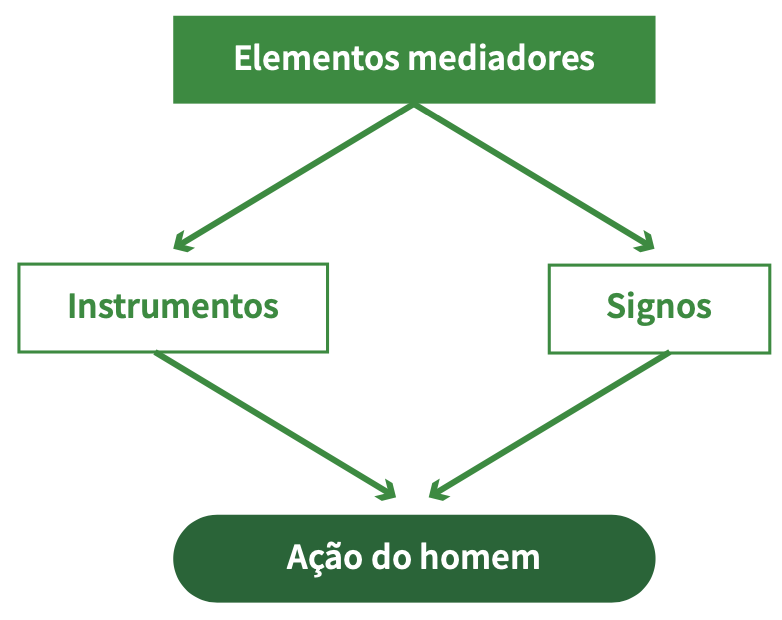
\includegraphics[scale=0.6]{figuras/elementos_mediadores.png}
    \label{fig:elementos_mediadores}
    \legend{Fonte: \citeonline{camillo2018teorias}}
\end{figure}

A mediação, segundo Vygotsky, é o processo pelo qual a ação do sujeito sobre o objeto é mediada por um determinado elemento. Por exemplo, a ação de um pintor sobre sua obra é mediada pelo pincel. Neste exemplo o elemento mediador (pincel) possibilita a transformação do objeto (quadro). Esta etapa intermediária “pincel -> quadro” é denominada mediação. Então, mediação é o processo de intervenção de um elemento intermediário numa relação - a relação deixa de ser direta e passa a ser mediada por esse elemento \cite{richit2004implicaccoes}.


Para Vygotsky as pessoas não tem um contato direto com objetos e sim uma mediação, por meio de um conhecimento ou por uma experiência, logo, ele defende a sua teoria como \textbf{sócio construtivista}, em que a interação é mediada por várias relações, vindo a se diferenciar do construtivismo, em que o indivíduo age sem desvios indo direto ao objetivo \cite{magalhaes2007perspectiva}.






Nesse sentido, \citeonline{ponte1988computador} acredita que os professores não devem deixar se reduzir ao papel de “correias de transmissão” de forma a utilizar em seu ensino produtos educacionais padronizados e prontos para usar.


Conforme citado por \citeonline{litto2009educaccao}, os novos modelos de aprendizagem utilizam intensamente as TIC e coincidem com a inovação em todos os níveis da vida humana. As novas tecnologias inserem-se no meio em que vivemos atualmente, o que impulsiona um conhecimento cada vez mais amplo, e por isso devemos utilizá-las como instrumento auxiliar no processo de ensino-aprendizagem. Nesse sentido \cite{richit2004implicaccoes}:

\begin{citacao}
Nesta perspectiva, a interferência da escola faz-se necessária no sentido de oferecer ao aluno oportunidades significativas de construção de conhecimentos e valores que estão atrelados à atual conjuntura social e, principalmente, promovendo a utilização das tecnologias informáticas como instrumentos auxiliares à prática pedagógica com o objetivo de promover interação, cooperação, comunicação e motivação a fim de diversificar e potencializar as relações inter e intrapessoais mediante situações mediatizadas, que venham a dar um novo significado ao processo de aprendizagem. Isto é, as relações entre sujeitos e, entre sujeitos e tecnologias colabora para a estruturação do conhecimento do grupo que a utiliza, bem como para o desenvolvimento desses sujeitos, o que caracteriza o coletivo seres humanos com mídias, proposto por \citeonline{levy1993tecnologias}.
\end{citacao}

De acordo com \citeonline{pais2002tecnologias} as tecnologias digitais ou software devem ser ajustados à linguagem dos alunos, isto é, devem apresentar uma interface de fácil interação, determinando a necessidade de serem avaliados segundo padrões vistos não somente sob o ponto de vista do nível de cognição e do valor do \textit{feedback}, mas segundo padrões culturais do sujeito.

Portanto, se as tecnologias informáticas fazem parte do contexto do aluno, então, a interação entre ambos (indivíduo/computador) precisa ser investigada como forma de favorecer o aprendizado e contribuir à construção do conhecimento \cite{richit2004implicaccoes}.





\section{Base Nacional Comum Curricular e a Matemática}
\label{bncc_mat}

A Base Nacional Comum Curricular (BNCC) é um documento normativo que estabelece as aprendizagens essenciais e progressivas que todos os estudantes devem adquirir ao longo das etapas e modalidades da Educação Básica \cite{bncc}.


Conforme definido na Lei de Diretrizes e Bases da Educação Nacional (LDB, Lei nº 9.394/1996), a Base deve nortear os currículos dos sistemas e redes de ensino das Unidades Federativas, como também as propostas pedagógicas de todas as escolas públicas e privadas de Educação Infantil, Ensino Fundamental e Ensino Médio, em todo o Brasil \cite{bncc}.

A Base estabelece conhecimentos, competências e habilidades que se espera que todos os estudantes desenvolvam ao longo da escolaridade básica. Orientada pelos princípios éticos, políticos e estéticos traçados pelas Diretrizes Curriculares Nacionais da Educação Básica, a Base soma-se aos propósitos que direcionam a educação brasileira para a formação humana integral e para a construção de uma sociedade justa, democrática e inclusiva \cite{bncc}.





%\section{Metodologias Ativas e Inovadoras na Educação}
%\label{metodologias_ativas}


%Diante árdua tarefa de dinamizar a prática docente, \citeonline{hartwig2019metodologias} afirmam que as metodologias ativas, em especial o ensino híbrido, com a ajuda dessas ferramentas síncronas e assíncronas, está sendo inserida nos sistemas educacionais, buscando inovar e ampliar a criatividade e a motivação.

%Conforme \citeonline{bacich2015aprender}, versar acerca de metodologias ativas implica partir do pressuposto de que não há um único modo de ensinar e de aprender. \citeonline{moran2015mudando} recomenda que as metodologias ativas sejam: “[...] pontos de partida para avançar para processos mais avançados de reflexão, de integração cognitiva, de generalização, de reelaboração de novas práticas”.

%Para \citeonline{barbosa2013metodologias} reforçam que, se a prática de ensino favorecer no estudante as ações de ouvir, ver, perguntar, discutir, fazer e ensinar, estar-se-á no caminho da aprendizagem ativa. De acordo com \citeonline{inocente2018metodologias}, utilizar metodologias ativas conduz a formação crítica de futuros profissionais, proporcionando o desenvolvimento de estudantes autônomos, criativos, críticos, interessados e firmes na tomada de decisões.



%\subsection{Gamificação no Ensino}
%\label{gamificicao}
%Do inglês “gamification”, a expressão gamificação foi assim intitulada pelo autor \cite{pelling2011short} adquiriu notabilidade por volta de 2010 apesar de ter surgido nos anos iniciais de 2000. Esta, como uma estratégia inovadora para o ambiente educacional, visa permitir uma vasta utilização de elementos e técnicas identificados e demasiadamente utilizados nos jogos no intuito de prover um cenário desafiador, obedecendo aos seguintes objetivos, mencionados por \cite{borges2013}, a saber:

%\begin{citacao}
%(1) aprimorar determinadas habilidades; (2) propor desafios que dão propósito/contexto a aprendizagem; (3)
%engajar os alunos em atividades mais participativas, interativas e interessantes; (4) maximizar o aprendizado de um determinado conteúdo; (5) promover a mudança de comportamento premiando ações adequadas e penalizando as inadequadas; (6) oferecer mecanismos de socialização e aprendizagem em grupo; e, finalmente, (7) discutir os benefícios da gamificação na motivação dos alunos para propor soluções aos diversos problemas de aprendizagem.
%\end{citacao}


%Um dos principais objetivos da gamificação é despertar o interesse dos estudantes para o processo de ensino e aprendizagem \cite{fardo2013gamificaccao}. Para \citeonline{sales2017gamificaccao}, gamificar a sala de aula não significa necessariamente criar um game, ou colocar a turma para jogar na sala de aula, mas consiste em usar as mesmas estratégias, métodos e pensamentos e alguns elementos do design de games no ambiente de aprendizagem, a saber: interação, colaboração, feedback, fases, desafios, motivação, regras claras dentre outros. 
























\chapter{Metodologia}
\label{metodologia}




\section{Caracterização da Pesquisa}

O percurso metodológico caracteriza-se como uma pesquisa aplicada, com abordagem mista (quantitativa e qualitativa), de natureza exploratória e com análise predominantemente indutiva, aplicando métodos de análise documental envolvendo os planos de aula e ensino para verificar no planejamento docente a previsão de adoção de alguma ferramenta tecnológica educacional e ou a transdisciplinaridade. A baixo na Figura \ref{fig:classificacao_metodologica} um esquema da classificação metodológica da pesquisa:

\begin{figure}[h!]
    \caption{Classificação metodológica}
    \centering
    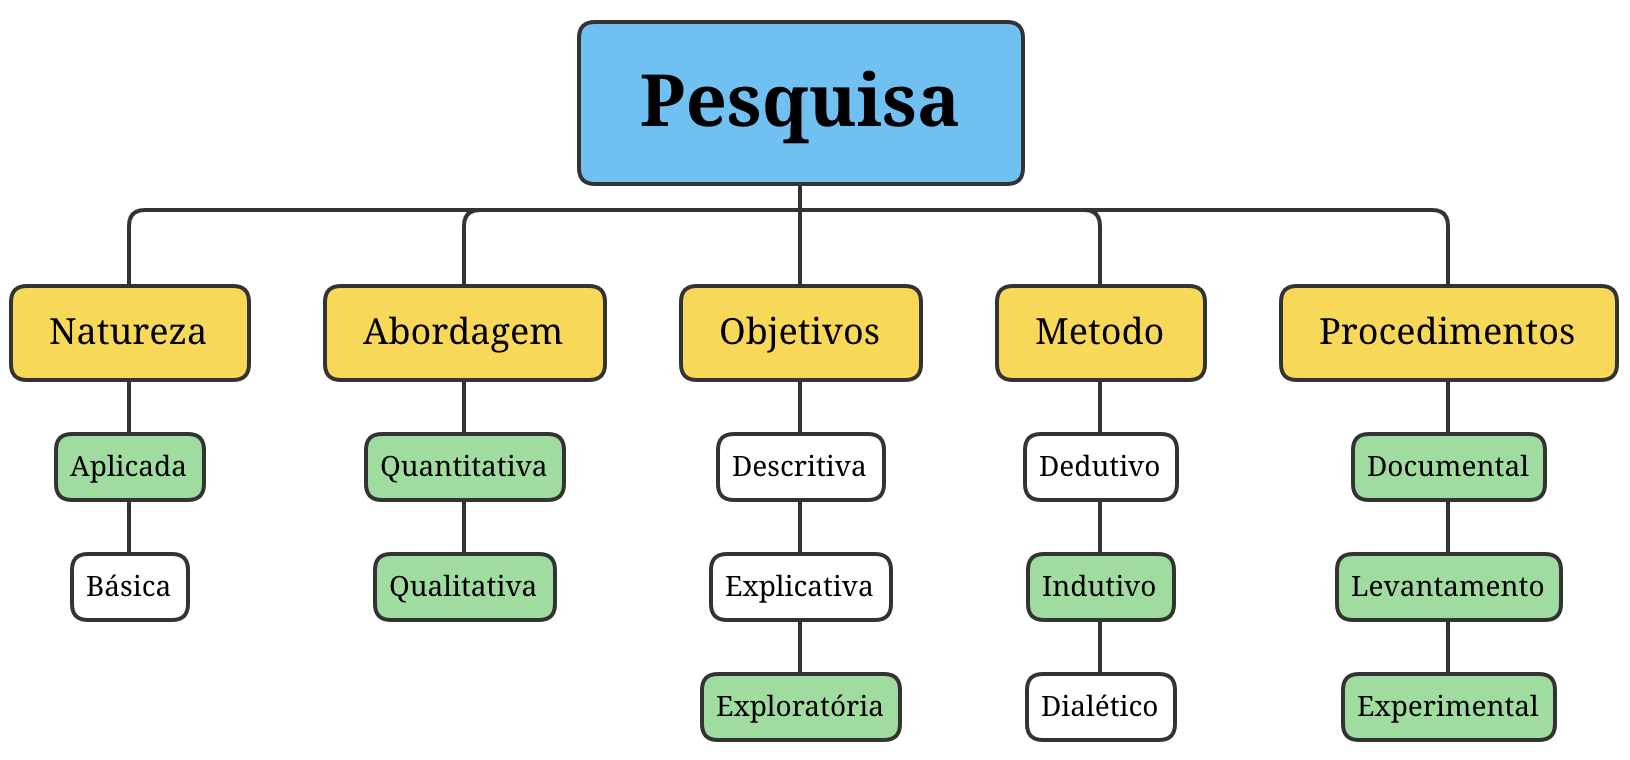
\includegraphics[scale=0.5]{figuras/metodologia.png}
    \label{fig:classificacao_metodologica}
    \legend{Fonte: Adaptado de \citeonline{marconi2017fundamentos}}
\end{figure}







\section{Local da Pesquisa}
\label{local_pesquisado}

O estudo foi conduzido no Instituto Federal do Amapá (IFAP), Campus Macapá, único campus da instituição que oferece o curso de Licenciatura em Matemática. O curso teve seu ato de criação pela Resolução nº 17/2016/CONSUP/IFAP, de 09 de maio de 2016 – Aprova o Ato de Criação, Autorização e Funcionamento do Curso Superior de Licenciatura em Matemática, modalidade presencial do Campus Macapá \cite{ifap2022}.

Também em 2016 publicou-se a Resolução nº 49/2016/CONSUP/IFAP, de 18 de outubro de 2016 – Aprova o Projeto Pedagógico do Curso Superior de Licenciatura em Matemática, modalidade presencial do Campus Macapá \cite{ifap2022}.









\section{Sujeitos da Pesquisa}
\label{sujeitos_pesquisa}

A população pesquisada será os docentes do curso, porém a amostragem corresponde apenas aos docentes que ministram os componentes não pedagógicos (componentes das áreas técnicas) totalizando 13 docentes, ressaltar que para acesso aos planos de aula e ensino deve-se adentrar ao Setor Pedagógico para obter acesso aos documentos e a busca fica restrita ao intervalo entre os anos de 2016 até 2021.


As informações serão coletadas por uma plataforma única para a coleta de dados ou utilizando um procedimento de amostragem em cadeia, como a metodologia conhecida como “bola de neve” (\textit{snowball sampling}) adaptada à plataformas virtuais \cite{szwarcwald2021convid}. O método “bola de neve” é um procedimento de amostragem não probabilístico, que funciona a partir da indicação de um grupo inicial de pessoas que fazem parte da população-alvo (denominadas de sementes), que indicam pares do mesmo grupo populacional, e assim sucessivamente, semelhante à formação de uma bola de neve \cite{szwarcwald2021convid}.





\subsection{Descrição dos Sujeitos}
\label{descricao_sujeitos}


Os docentes, sujeitos da pesquisa são caracterizados pelo eixo de disciplinas ligados ao curso de licenciatura em matemática de ambos os sexos e tempo de experiência diversos até mesmo em outras de áreas do conhecimento. Ressaltar que apenas os docentes do Campus Macapá que ministram componentes específicos da matemática inicialmente participaram indicando outros seguindo docentes seguindo o método da bola de neve.








\subsection{Critérios de Inclusão e Exclusão}
\label{criterios_sujeitos}

Como critérios de inclusão para todos os participantes  é dar o aceite concordando com o Termo de Esclarecimento Livre Esclarecido (TCLE):
\begin{itemize}
    \item Ser docente efetivo, substituto ou temporário do IFAP ou em instituição com o curso de Licenciatura em Matemática;
    \item Ministrar componentes no curso de Licenciatura em Matemática;
    \item Componente ministrado seja da área técnica ou superior;
    \item Atuado no período entre 2016 até 2021.
\end{itemize}




\section{Aspectos Éticos}
\label{aspectos_eticos}

Toda a pesquisa com seres humanos envolve um risco específico caracterizado como “dano”. Esse dano poderá ser “associado ou decorrente da pesquisa - agravo imediato ou posterior, direto ou indireto, ao indivíduo ou à coletividade, decorrente da pesquisa;”. \cite{cns466}.

O projeto de pesquisa tramitou e foi aprovado pelo Comitê de Ética em Pesquisa (CEP) via protocolo: 70930823.6.0000.0211 na Plataforma Brasil do Ministério da Saúde, segundo o \citeonline{cns510} o planejamento ou a execução da atividade de educação, ensino ou treinamento surja a intenção de incorporação dos resultados dessas atividades em um projeto de pesquisa, dever-se-á, de forma obrigatória, apresentar o protocolo de pesquisa ao sistema CEP/CONEP.

O processo de \textbf{consentimento} e do \textbf{assentimento} livre e esclarecido envolve o estabelecimento de relação de confiança entre pesquisador e participante, continuamente aberto ao diálogo e ao questionamento, podendo ser obtido ou registrado em qualquer das fases de execução da pesquisa, bem como retirado a qualquer momento, sem qualquer prejuízo ao participante \cite{cns510}.

Para garantia e atender às exigências éticas e científicas fundamentais para trabalhos de pesquisas com seres humanos, todos os participantes devem ser submetidos ao Termo de Consentimento Livre Esclarecido (TCLE). Entende-se por Processo de Consentimento Livre e Esclarecido todas as etapas a serem necessariamente observadas para que o convidado a participar de uma pesquisa possa se manifestar, de forma autônoma, consciente, livre e esclarecida \cite{cns466}.




\section{Riscos da Pesquisa}
\label{riscos_pesquisa}

A resolução do Conselho Nacional de Saúde (CNS) nº 466/12 versa que toda pesquisa com seres humanos envolve riscos nas dimensões física, psíquica, moral, intelectual, emocional, social, cultural ou espiritual do ser humano, em tipos e gradações variadas, mesmo que mínimas. Assim para participação deve-se aplicar o TCLE a todos os interessados a colaborar de forma espontânea.


Segue alguns possíveis riscos da pesquisa, como a possibilidade de constrangimento, disponibilidade de tempo para responder ao instrumento de pesquisa, alterações de comportamento natural, exposição de dados do participante que possam resultar na sua identificação. Outro ponto é relacionado ao desconforto emocional relacionado a presença do pesquisador. Outro ponto é com relação a possíveis desconfortos e constrangimentos quando há falta de cuidado na elaboração do conteúdo e no modo de aplicação.






\section{Benefícios da Pesquisa}
\label{beneficios_pesquisa}

Em consonância com os objetivos supracitados e em corroboração com a proposta de análise das práticas docentes no uso das ferramentas auxiliares para mediação de conteúdos de matrizes, se propõem um produto funcional para uso em sala ou remoto, além de integrar ferramentas tecnológicas livres e reutilizáveis em outras esferas, consolidando de forma atrativa o ensino-aprendizagem como a construção de modelos visuais dinâmicos de interação e integração. 

Um dos resultados da pesquisa é um artefato digital como Recurso Educacional Aberto (REA) que assegura a reutilização deste produto educacional desenvolvido na pesquisa para futuros trabalhos e melhorias, garantindo a aplicação e reprodução livre. A possibilidade de adoção e ou investimento na expansão de funcionalidades no Produto Mínimo Viável (PMV) apresentado que poderá ser registrado como programa de computador via Núcleo de Inovação Tecnológica (NIT) ou outras plataformas de REA.






\section{Instrumentos de Pesquisa}
\label{instrumentos}

O levantamento de dados desta pesquisa envolveu a aplicação de questionários e entrevistas estruturadas, visando coletar informações detalhadas dos participantes

O levantamento de dados desta pesquisa envolveu variadas fontes, visando coletar informações detalhadas dos participantes aplicando métodos ou técnicas da academia. Esse material-fonte geral é útil não apenas por trazer conhecimentos que servem de \textit{background} ao campo de interesse, como também para evitar possíveis duplicações e/ou esforços desnecessários; pode, ainda, sugerir problemas e hipóteses além de orientar para outras fontes de coleta \cite{marconi2017fundamentos}.

O levantamento de dados é a fase da pesquisa realizada com intuito de recolher informações prévias sobre o campo de interesse. Ele se constitui de um dos primeiros passos de qualquer pesquisa científica e foi feito de duas maneiras: pesquisa documental (ou de fontes primárias) e pesquisa bibliográfica (ou de fontes secundárias) \cite{marconi2017fundamentos}.

Outro instrumento utilizado para coleta dos dados é o questionário eletrônico com perguntas abertas e fechadas divididos em dois momentos. A analise dos dados seguirão o método de analise de conteúdo com consolidação dos dados tabulados em gráficos e categorias. As etapas abaixo seguem como guia para elucidar ações a serem desenvolvidas:

\begin{enumerate}
    \item Termo de Anuência Institucional do local de pesquisa autorizando;
    \item Submissão do projeto junto ao comitê de ética em pesquisa (CEP) via Plataforma Brasil;
    \item Pesquisa e análise documental;
    \item Etapa de Diagnóstico: Questionário Pré Diagnóstico e Sócio Tecnológico.
    \item Etapa de Intervenção: Questionário de Avaliação de Experiência do usuário, Interface para usuário;
    \item Etapa de Consolidação e Resultados: Questionário de Avaliação da Proposta de Ferramenta (produto educacional).
\end{enumerate}




\subsection{Análise e Interpretação dos Dados}
\label{analise_dados}

Para \citeonline{best1972investigar}, a análise e interpretação "representa aplicação lógica dedutiva e indutiva do processo de investigação". Os dados e informações levantados proporcionam respostas às investigações pela sua importância no contexto local que a caracteriza. A Figura \ref{fig:tipos_analise_dados} demonstra que a Análise e Interpretação são duas atividades distintas, mas extremamente relacionadas e, como processo, envolvem duas operações \cite{marconi2017fundamentos}.

\begin{figure}[h!]
    \caption{Tipos de Análise de dados}
    \centering
    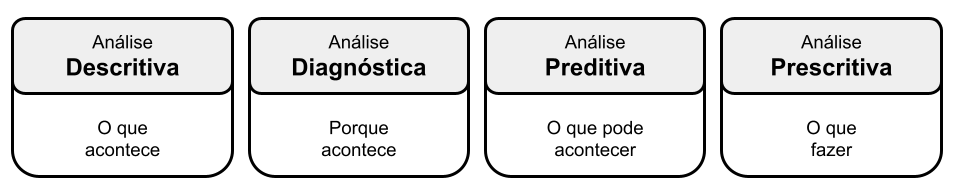
\includegraphics[scale=0.4]{figuras/tipos_analise_dados.png}
    \label{fig:tipos_analise_dados}
    \legend{Fonte: Adaptado de \citeonline{marquesone2016big}.}
\end{figure}


Essencialmente, as análises de dados podem ser divididas em quatro finalidades distintas: descritivas, diagnósticas, preditivas e prescritivas \cite{marquesone2016big}, ilustrada na Figura \ref{fig:tipos_analise_dados}. Foi aplicado a análise descritiva para dizer o que de fato acontece para na tentativa de entender o porque acontece, assim como a análise preditiva como previsão do que pode acorrer ou ocorre, tomando como referência dados reais coletados de forma indutiva para guiar na ação do que fazer, direcionando as etapas seguintes.

O processo de análise de dados é composto por seis etapas essenciais conforme a Figura \ref{fig:processo_analise_dados}, considerando o objeto tema de análise e algumas ferramentas (Google Forms\footnote{https://forms.google.com} e Survio\footnote{https://survio.com}) foram aplicadas para o processo de coleta, tabulação e análise.

\begin{figure}[h!]
    \caption{Processo de Análise de dados}
    \centering
    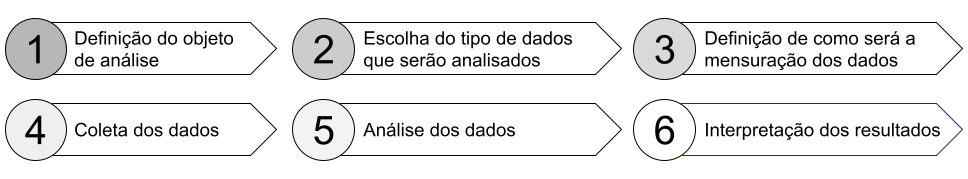
\includegraphics[scale=0.45]{figuras/processo_analise_dados.png}
    \label{fig:processo_analise_dados}
    \legend{Fonte: Adaptado de \citeonline{marquesone2016big}.}
\end{figure}

A análise utilizou para avaliar os dados encadeados nos documentos como Planos de Aula, Plano de Ensino, Plano Pedagógico de Curso (PPC) e outros documentos pertinentes como projetos interdisciplinares ou integradores e dos questionários aplicados. Por fim para \cite{marconi2017fundamentos} esta análise se divide em três etapas, compreendidas entre "interpretação, explicação e especificação", considerando cada aspecto pontual e ou categorizado.
\chapter{Resultados}
\label{resultados}



\section{Pré Diagnóstico e Sócio Tecnológico}
\label{pre_diagnostico_socio_tec}

No total, participaram oito docentes do universo populacional pesquisado, sendo 37,5\% mulheres e 62,5\% homens, conforme ilustrado na Figura \ref{fig:genero_participantes}. Embora tenha ocorrido um aumento no ingresso de mulheres no ensino superior, sua presença nos cursos de matemática e estatística permanece reduzida. Essa realidade é destacada em um boletim divulgado em 12 de maio de 2023 pela Sociedade Brasileira de Matemática (SBM) e pela Sociedade Brasileira de Matemática Aplicada e Computacional (SBMac), em colaboração com a Associação Brasileira de Estatística, que reforça a sub-representação feminina nessas áreas.

\begin{figure}[h!]
    \caption{Gênero dos Participantes}
    \centering
    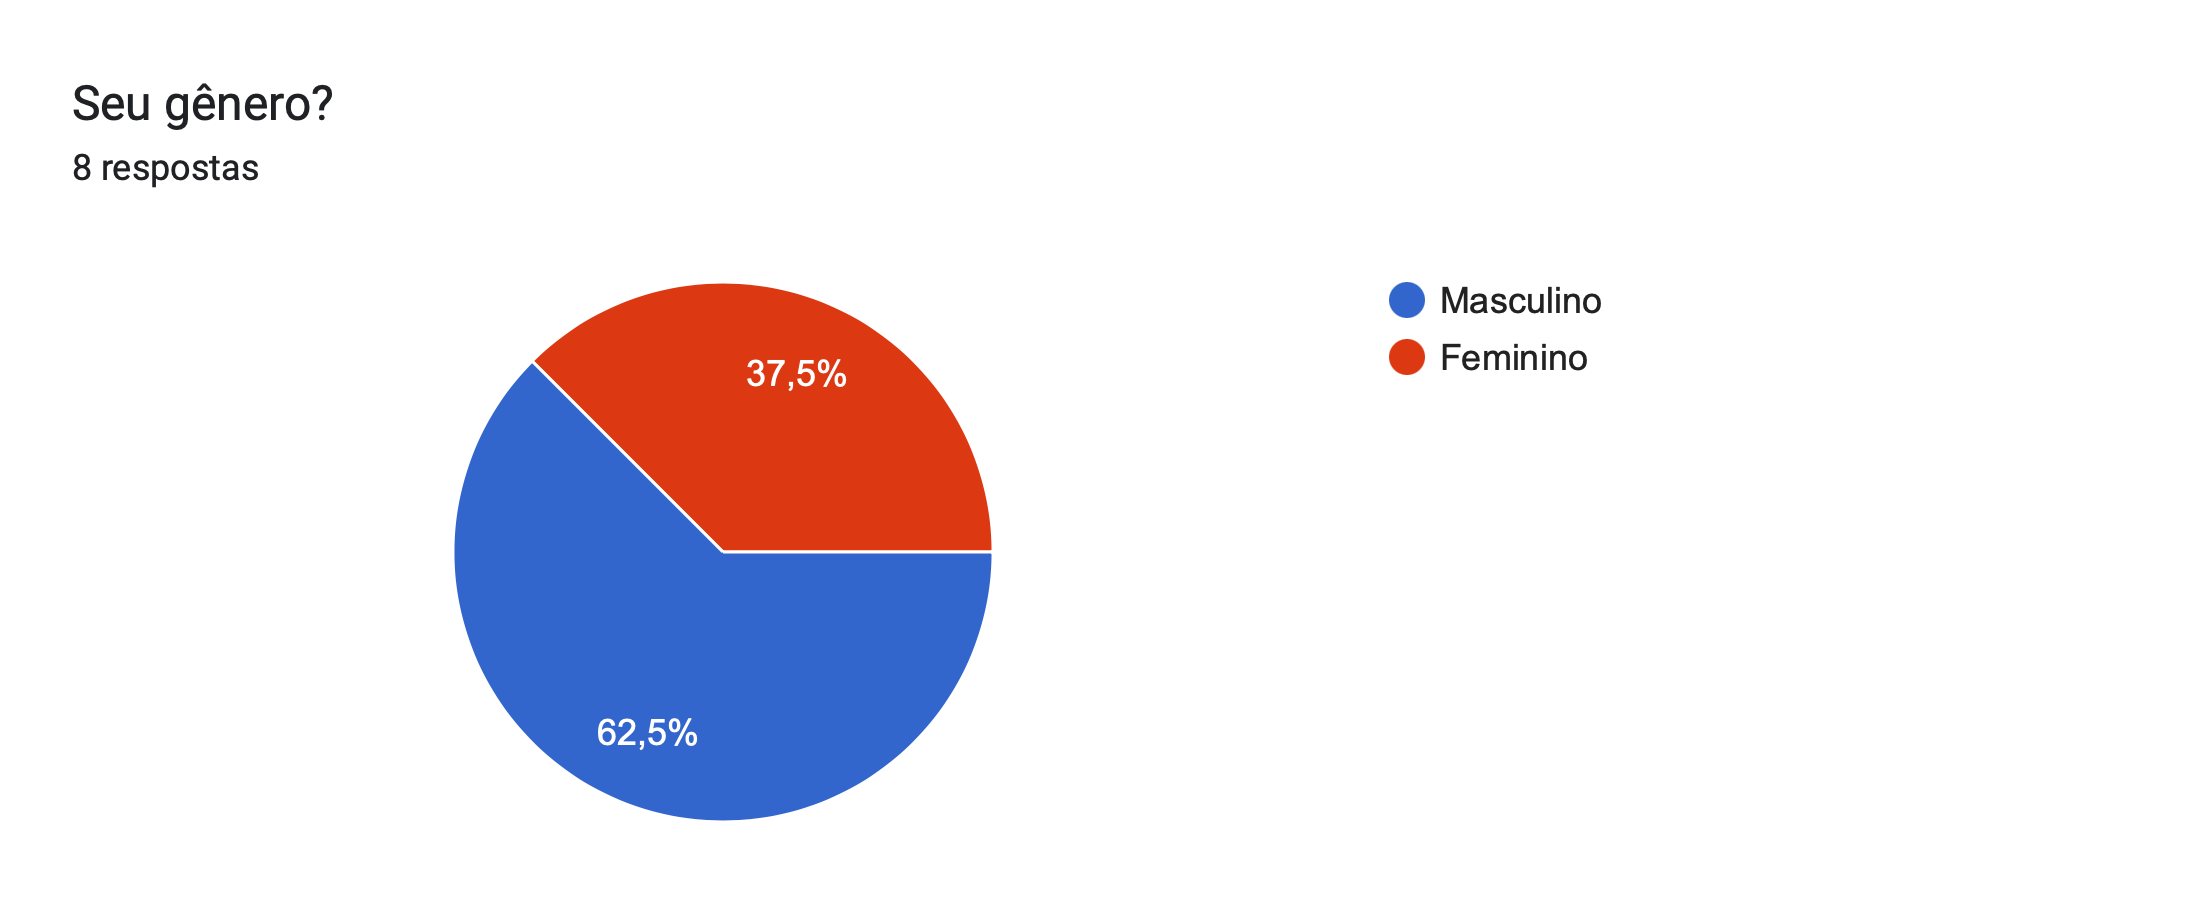
\includegraphics[scale=0.2]{figuras/resultados/genero.png}
    \label{fig:genero_participantes}
    \legend{Fonte: Eonay e Klenilmar (2024).}
\end{figure}

A participação das mulheres nas ciências exatas, embora crescente, ainda enfrenta desafios significativos, especialmente em áreas como matemática, estatística e física. Estudos indicam que fatores históricos, culturais e sociais têm contribuído para a sub-representação feminina nesses campos, perpetuando estereótipos de gênero que desencorajam sua inserção. Segundo um levantamento da \cite{brasil2018decifrar}, as mulheres representam apenas cerca de 30\% dos pesquisadores em áreas STEM (Ciência, Tecnologia, Engenharia e Matemática) no mundo.

No Brasil, conforme aponta o boletim da Sociedade Brasileira de Matemática (SBM) e da Sociedade Brasileira de Matemática Aplicada e Computacional (SBMac) de 2023, a disparidade é evidente nos cursos de matemática e estatística, que continuam sendo predominantemente masculinos. Promover iniciativas de inclusão e destacar modelos femininos de sucesso são estratégias fundamentais para equilibrar essa desigualdade e estimular novas gerações de mulheres a ingressarem e se destacarem nas ciências exatas.



Um aspecto analisado no estudo foi a experiência docente relacionada ao ensino do conteúdo de matrizes, uma estrutura amplamente utilizada em diversas disciplinas e áreas do conhecimento. Os dados revelam que 62,5\% dos participantes afirmaram já ter trabalhado diretamente com o tema, enquanto 37,5\% indicaram ainda não tê-lo abordado, como ilustrado na Figura \ref{fig:trabalhou_matrizes}. O uso de matrizes é essencial em áreas como matemática aplicada, estatística e ciência de dados, destacando sua relevância na formação acadêmica e interdisciplinar \cite{golub2013matrix}.

\begin{figure}[h!]
    \caption{Trabalhou diretamente com o conteúdo de Matrizes}
    \centering
    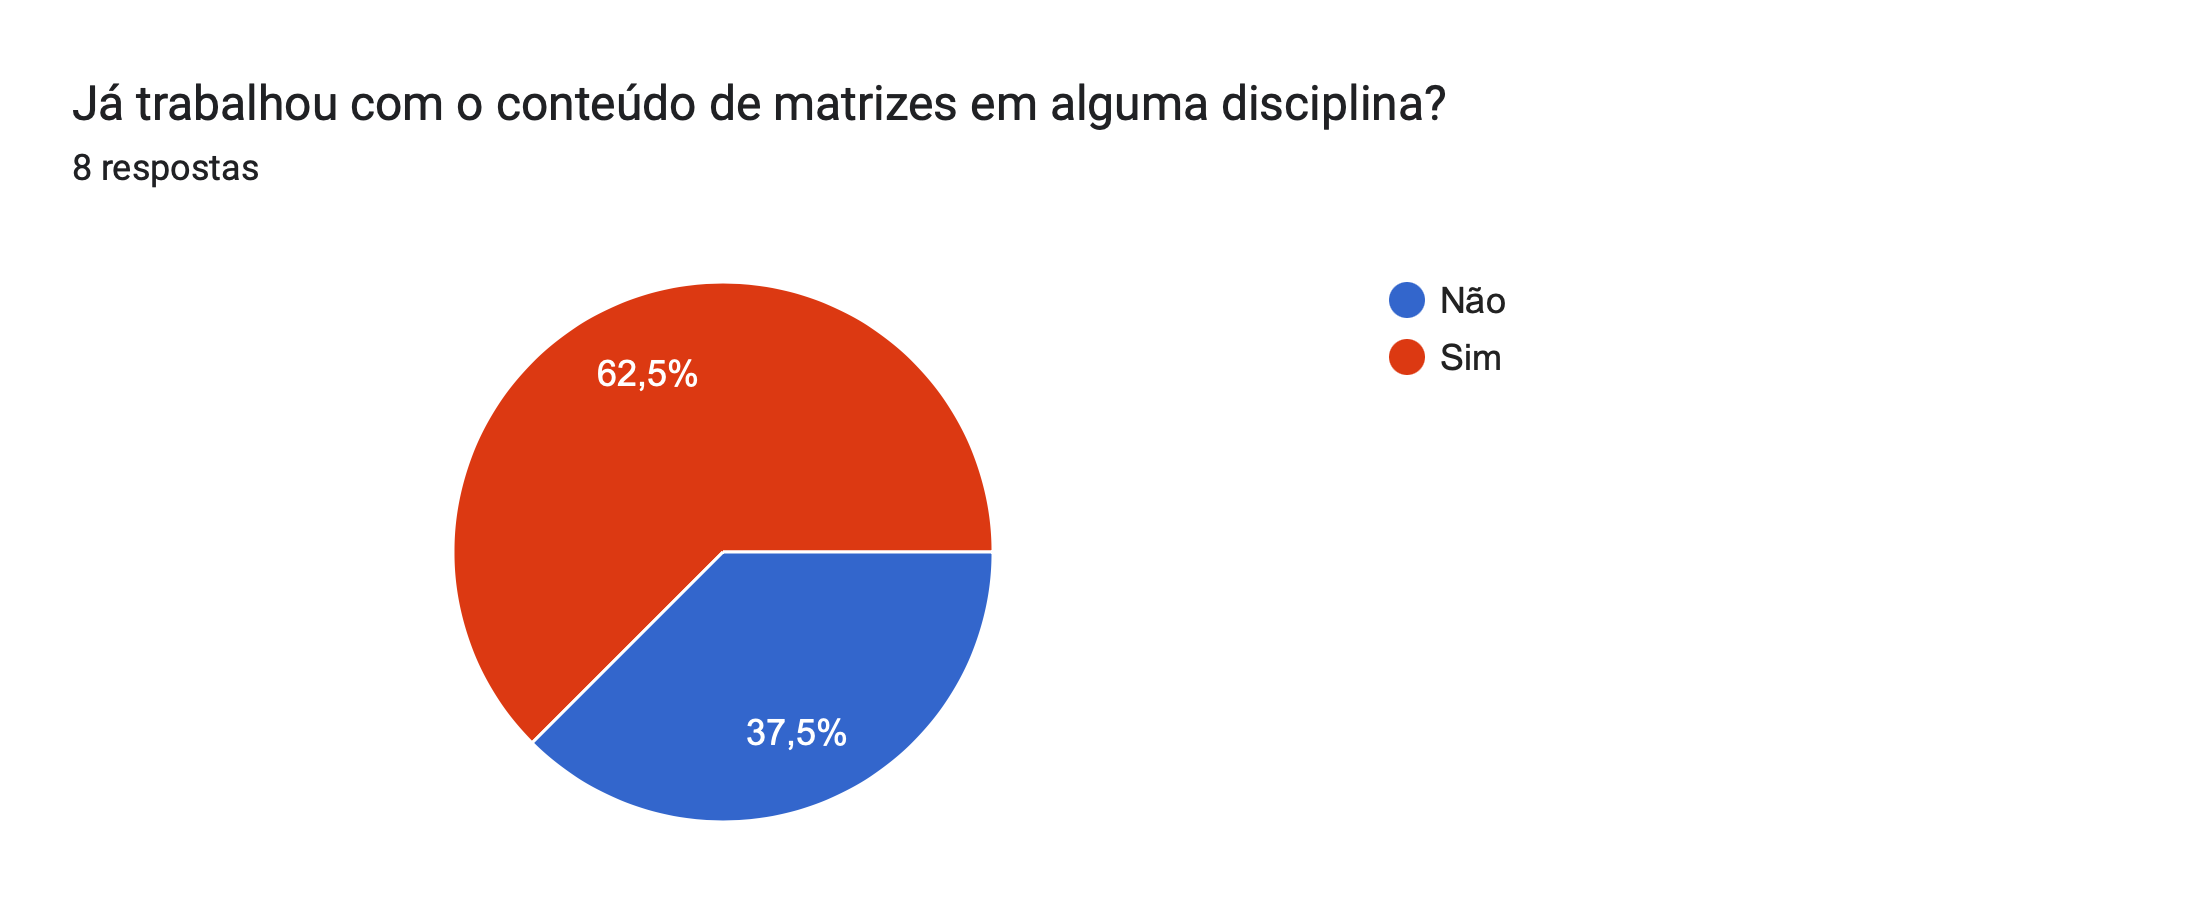
\includegraphics[scale=0.2]{figuras/resultados/trabalhou_matrizes.png}
    \label{fig:trabalhou_matrizes}
    \legend{Fonte: Eonay e Klenilmar (2024).}
\end{figure}

Aos participantes que já trabalharam com o conteúdo sobre matrizes, foi solicitado optativamente que informassem quais as disciplinas trabalhadas, assim obteve-se o resultado abaixo:

\begin{citacao}
    \item "Matemática para ensino médio, e superior. Conteúdo estritamente teórico";
    \item "Matemática 2ª série E.M";
    \item "Álgebra Linear, Matemática no 2º ano do Ensino Médio";
    \item "Matemática, Geometria Analítica e Vetores";
    \item "Matemática".
\end{citacao}
    

As disciplinas mencionadas reforçam a ideia de que a estrutura de matrizes pode e deve ser integrada ao ensino de outras áreas, evidenciando sua aplicabilidade interdisciplinar e sua utilização frequente em atividades realizadas em sala de aula. Além disso, foi investigado um aspecto tecnológico relacionado ao acesso à internet, conforme apresentado na Figura \ref{fig:acesso_internet}, destacando sua relevância para o ensino e aprendizagem nos contextos atuais.

\begin{figure}[h!]
    \caption{Acesso a Internet}
    \centering
    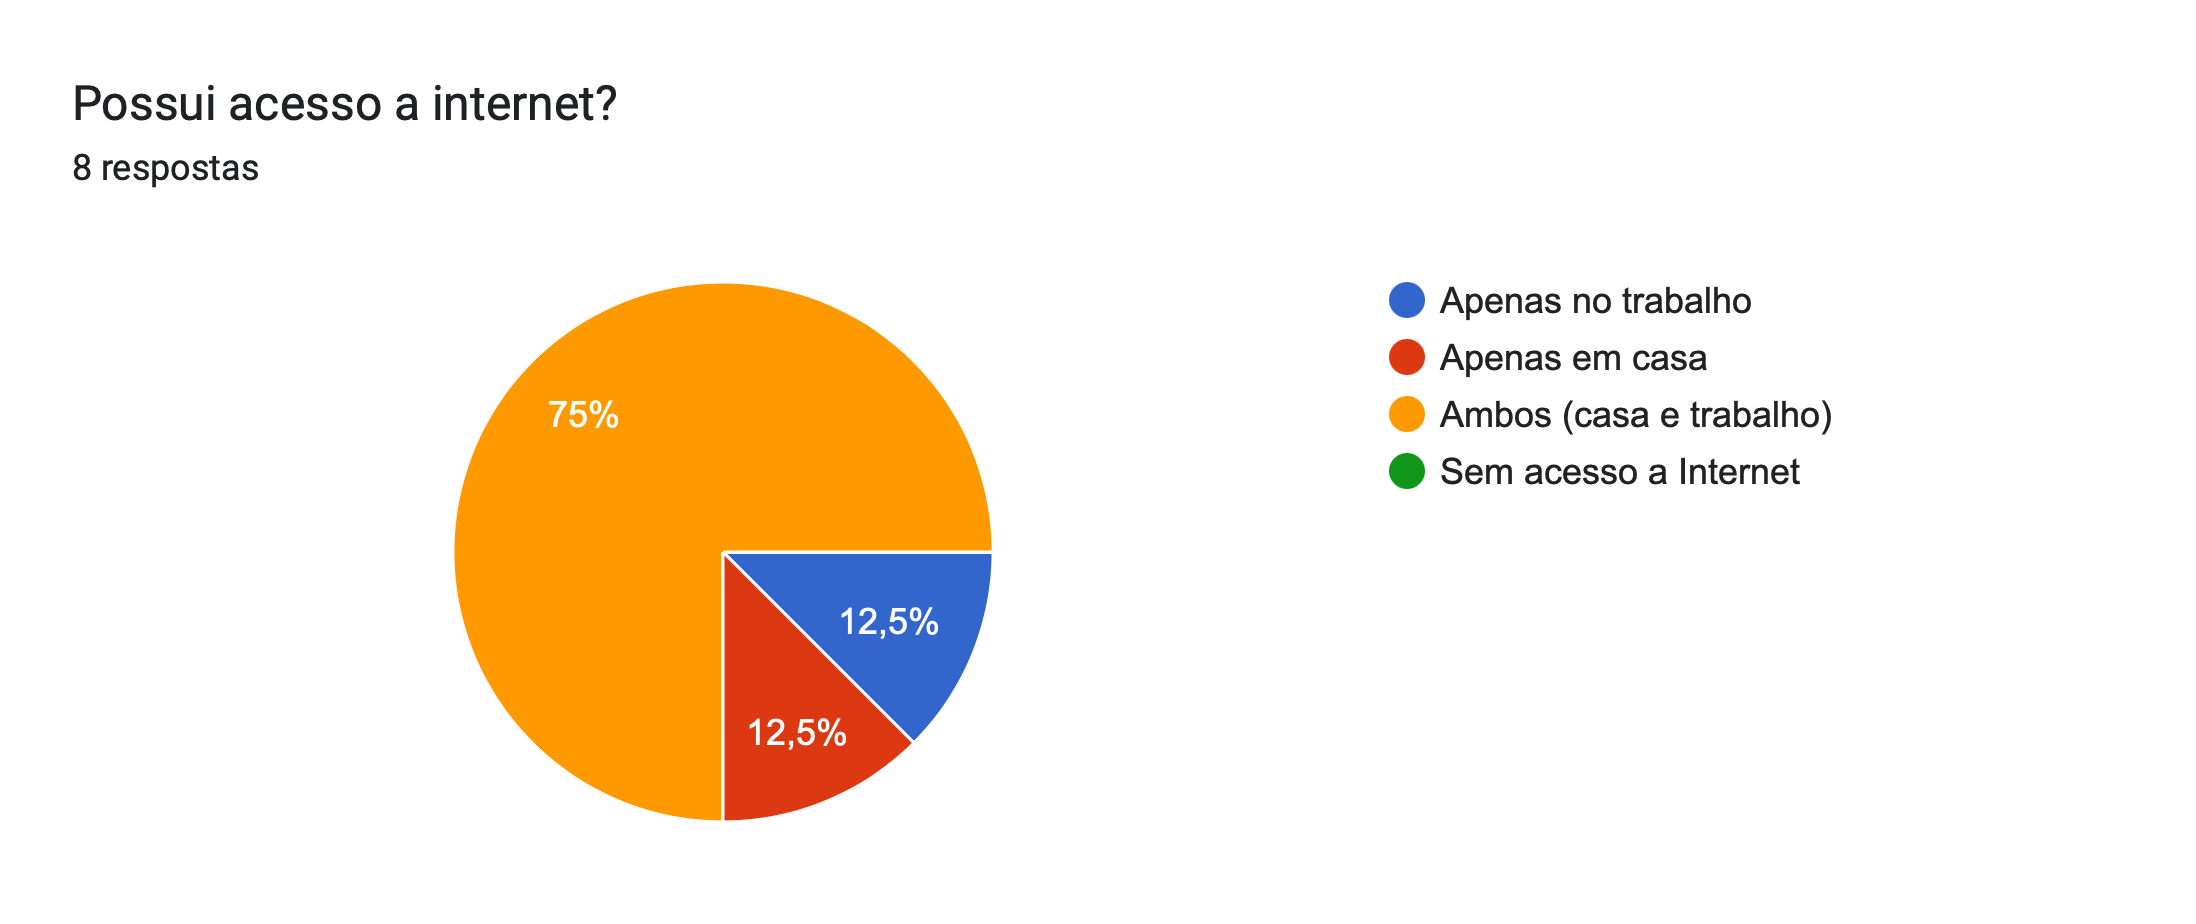
\includegraphics[scale=0.2]{figuras/resultados/acesso_internet.png}
    \label{fig:acesso_internet}
    \legend{Fonte: Eonay e Klenilmar (2024).}
\end{figure}

Para o uso da internet na prática docente podemos constatar que o acesso é de alcance a todos participantes seja ele no trabalho (12,5\%), em casa (12,5\%) ou ambos (75,0\%) os locais. Também foi levantado os dados do tipo de dispositivos que mais se utiliza para acesso a internet, onde representou 75,0\% o computador portátil. Também se tratando de portabilidade os \textit{smartphones} e \textit{tablets} também citados cada um com 12,5\% como dispositivos preferidos para esse uso, segue Figura \ref{fig:dispositivo_acesso_internet} com os referidos resultados.

\begin{figure}[h!]
    \caption{Dispositivo de acesso a Internet}
    \centering
    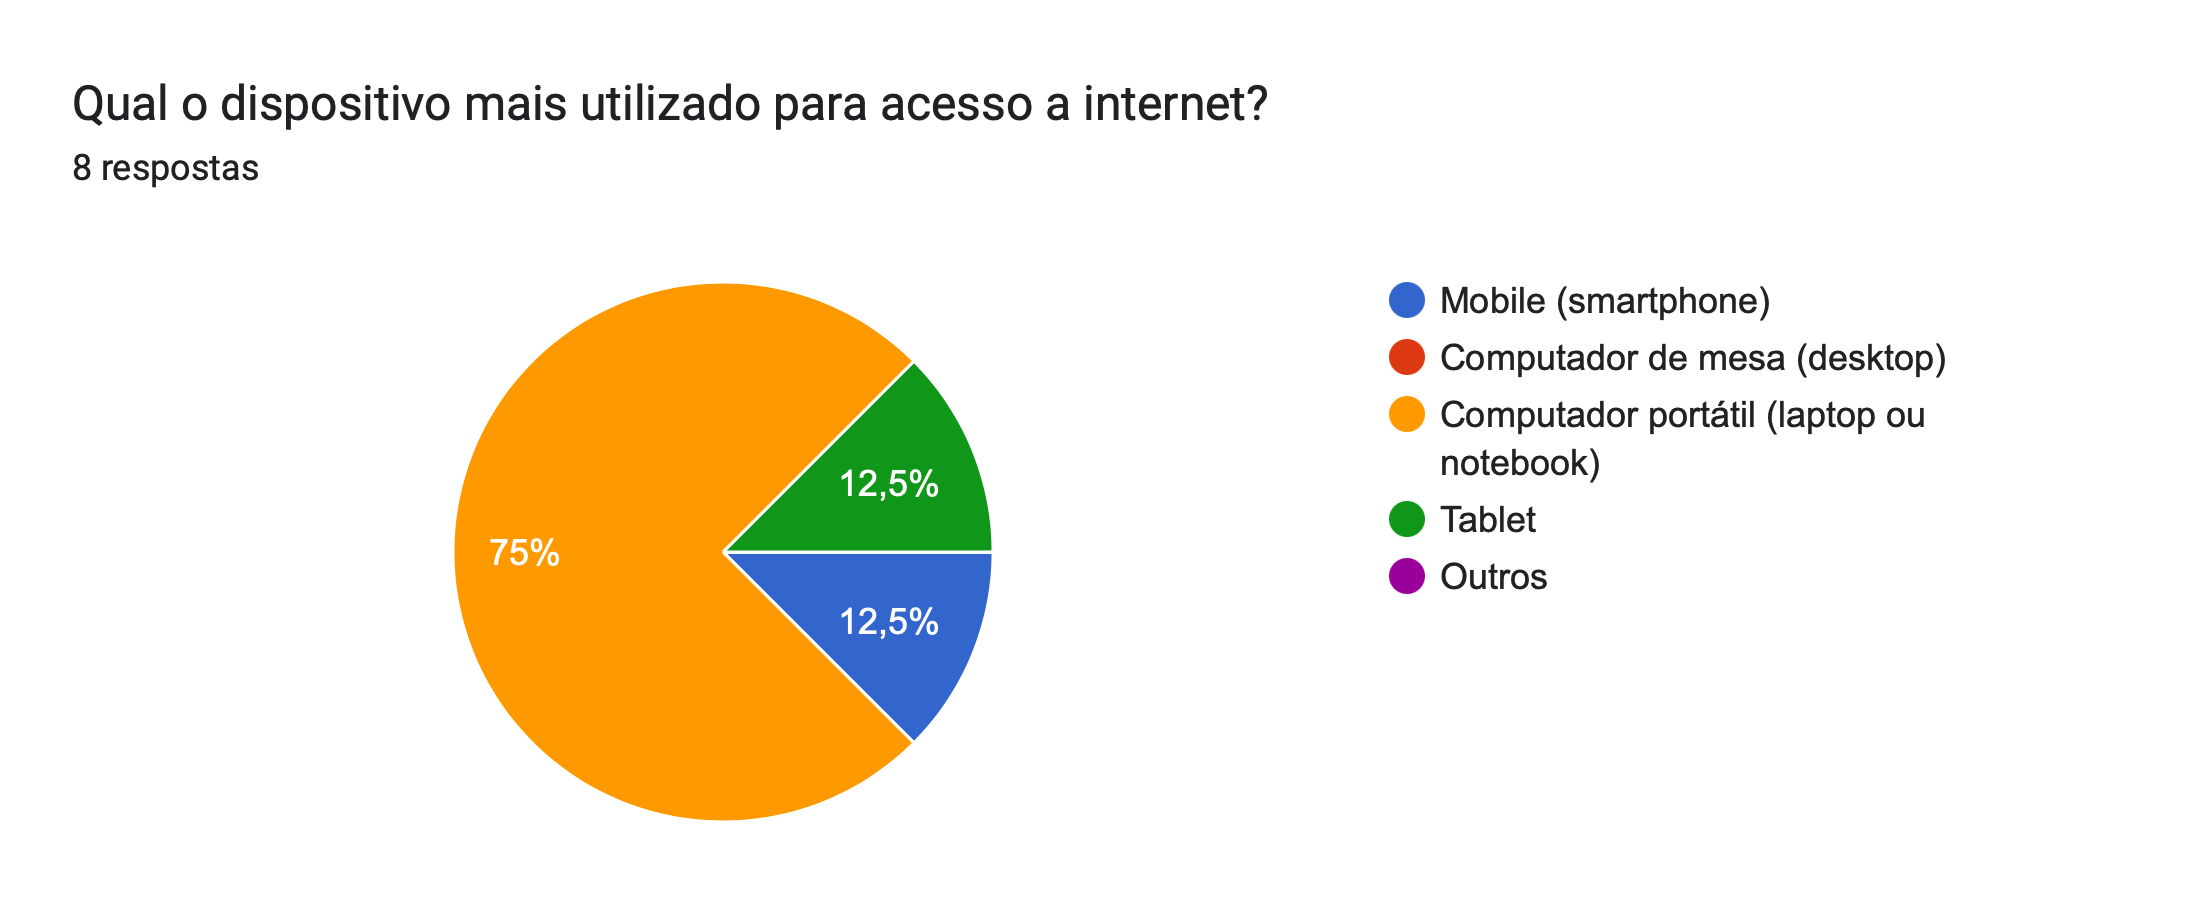
\includegraphics[scale=0.2]{figuras/resultados/dispositivo_acesso_internet.png}
    \label{fig:dispositivo_acesso_internet}
    \legend{Fonte: Eonay e Klenilmar (2024).}
\end{figure}



Considerando o uso das redes mundiais de computadores ou mais conhecida como a Internet, os principais dispositivos utilizados são os  móveis conforme indicativos supracitados é natural a utilização de softwares ou aplicativos para auxiliar a prática docente. O indicativo levantado direcionado a medir a frequência que se aplica tecnologias nos ambientes de ensino representado na Figura \ref{fig:softs_docencia}.

\begin{figure}[h!]
    \caption{Utilização de Softwares ou Aplicativos na Prática Docente}
    \centering
    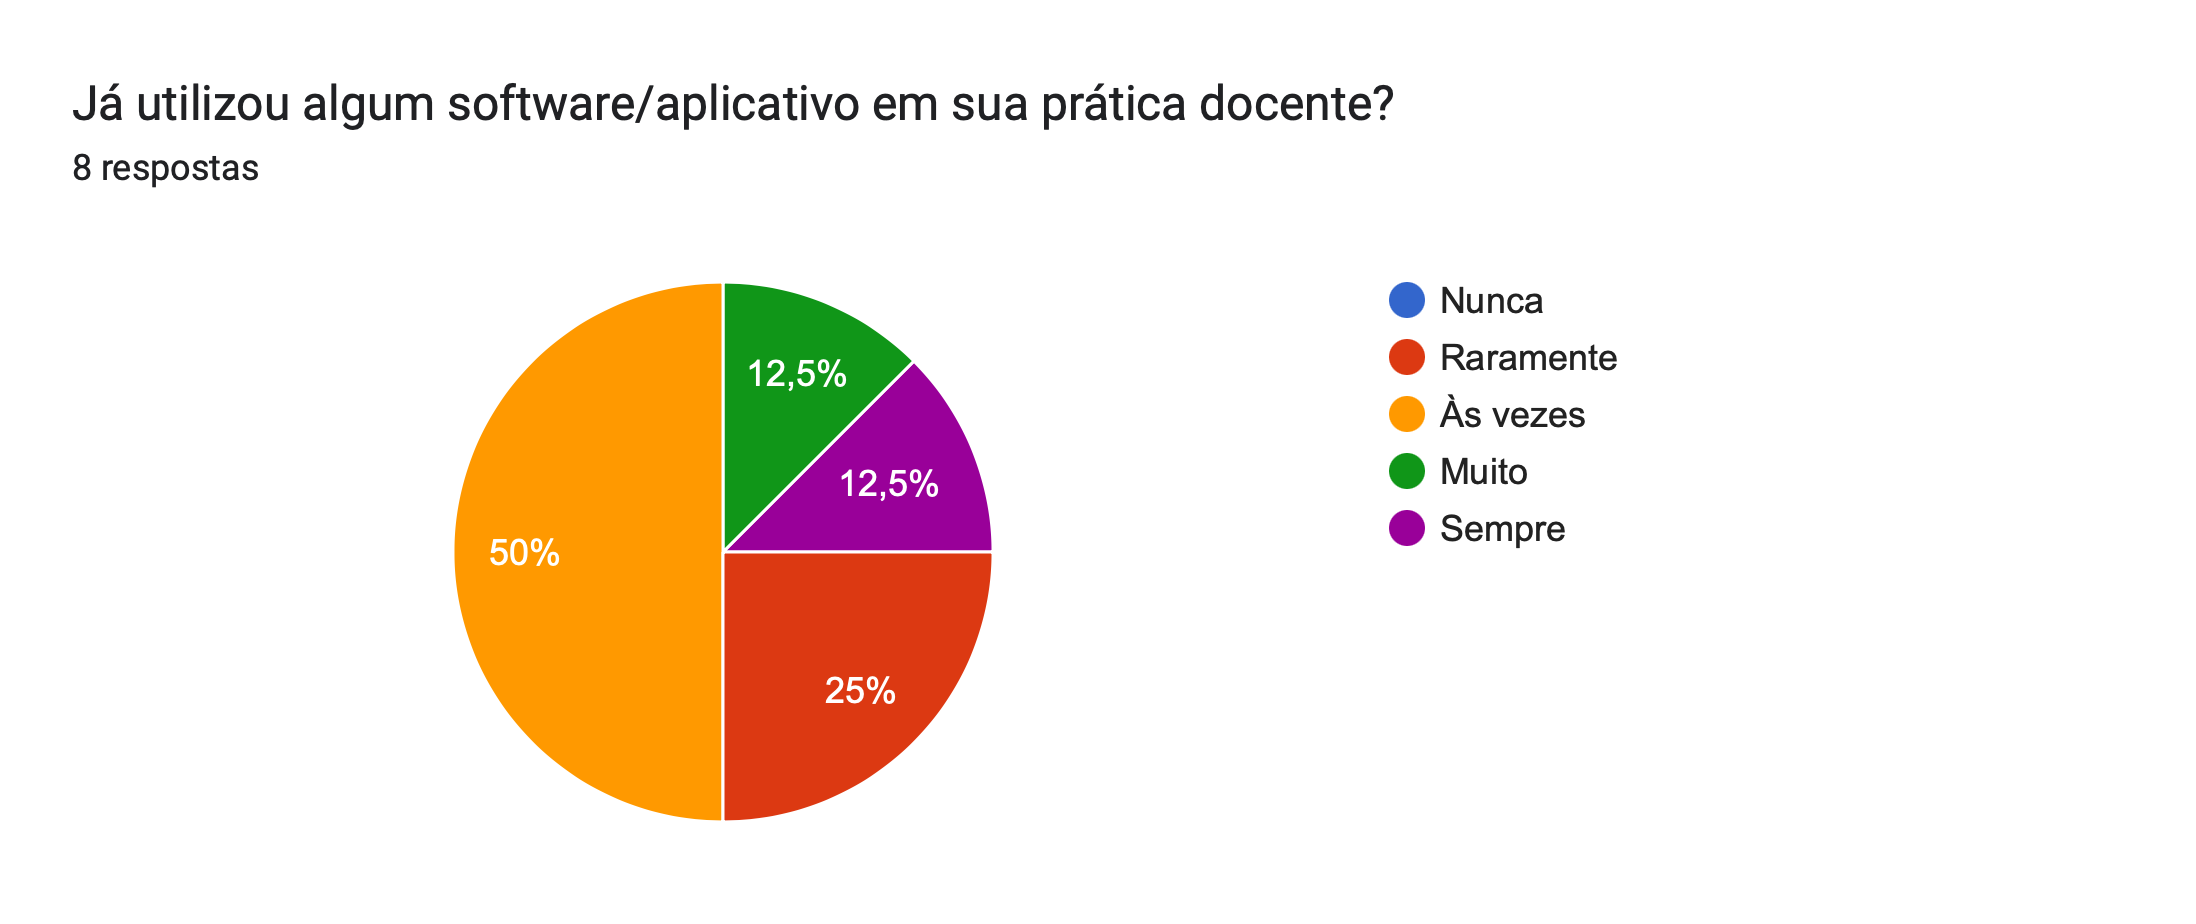
\includegraphics[scale=0.2]{figuras/resultados/software_pratica_docente.png}
    \label{fig:softs_docencia}
    \legend{Fonte: Eonay e Klenilmar (2024).}
\end{figure}



A análise do uso de ferramentas na prática docente revelou que 25,0\% dos participantes relataram utilizá-las raramente, enquanto 12,5\% afirmaram usá-las com frequência (muito) ou de forma constante (sempre) em suas aulas. A maioria, equivalente a 50,0\%, indicou utilizá-las apenas ocasionalmente (às vezes). Esses dados sugerem um indicativo de baixo uso de ferramentas tecnológicas nessa abordagem inicial e direcionada.

Quando questionados diretamente sobre a possibilidade de ensinar o conteúdo básico de matrizes utilizando alguma ferramenta tecnológica, 75,0\% dos educadores demonstraram concordância, enquanto 25,0\% preferiram se abster de responder, conforme ilustrado na Figura \ref{fig:ensino_matriz_app}. Esses resultados apontam para um potencial ainda pouco explorado no uso de ferramentas para o ensino desse conteúdo.

\begin{figure}[h!]
    \caption{Ensinar matriz utilizando software}
    \centering
    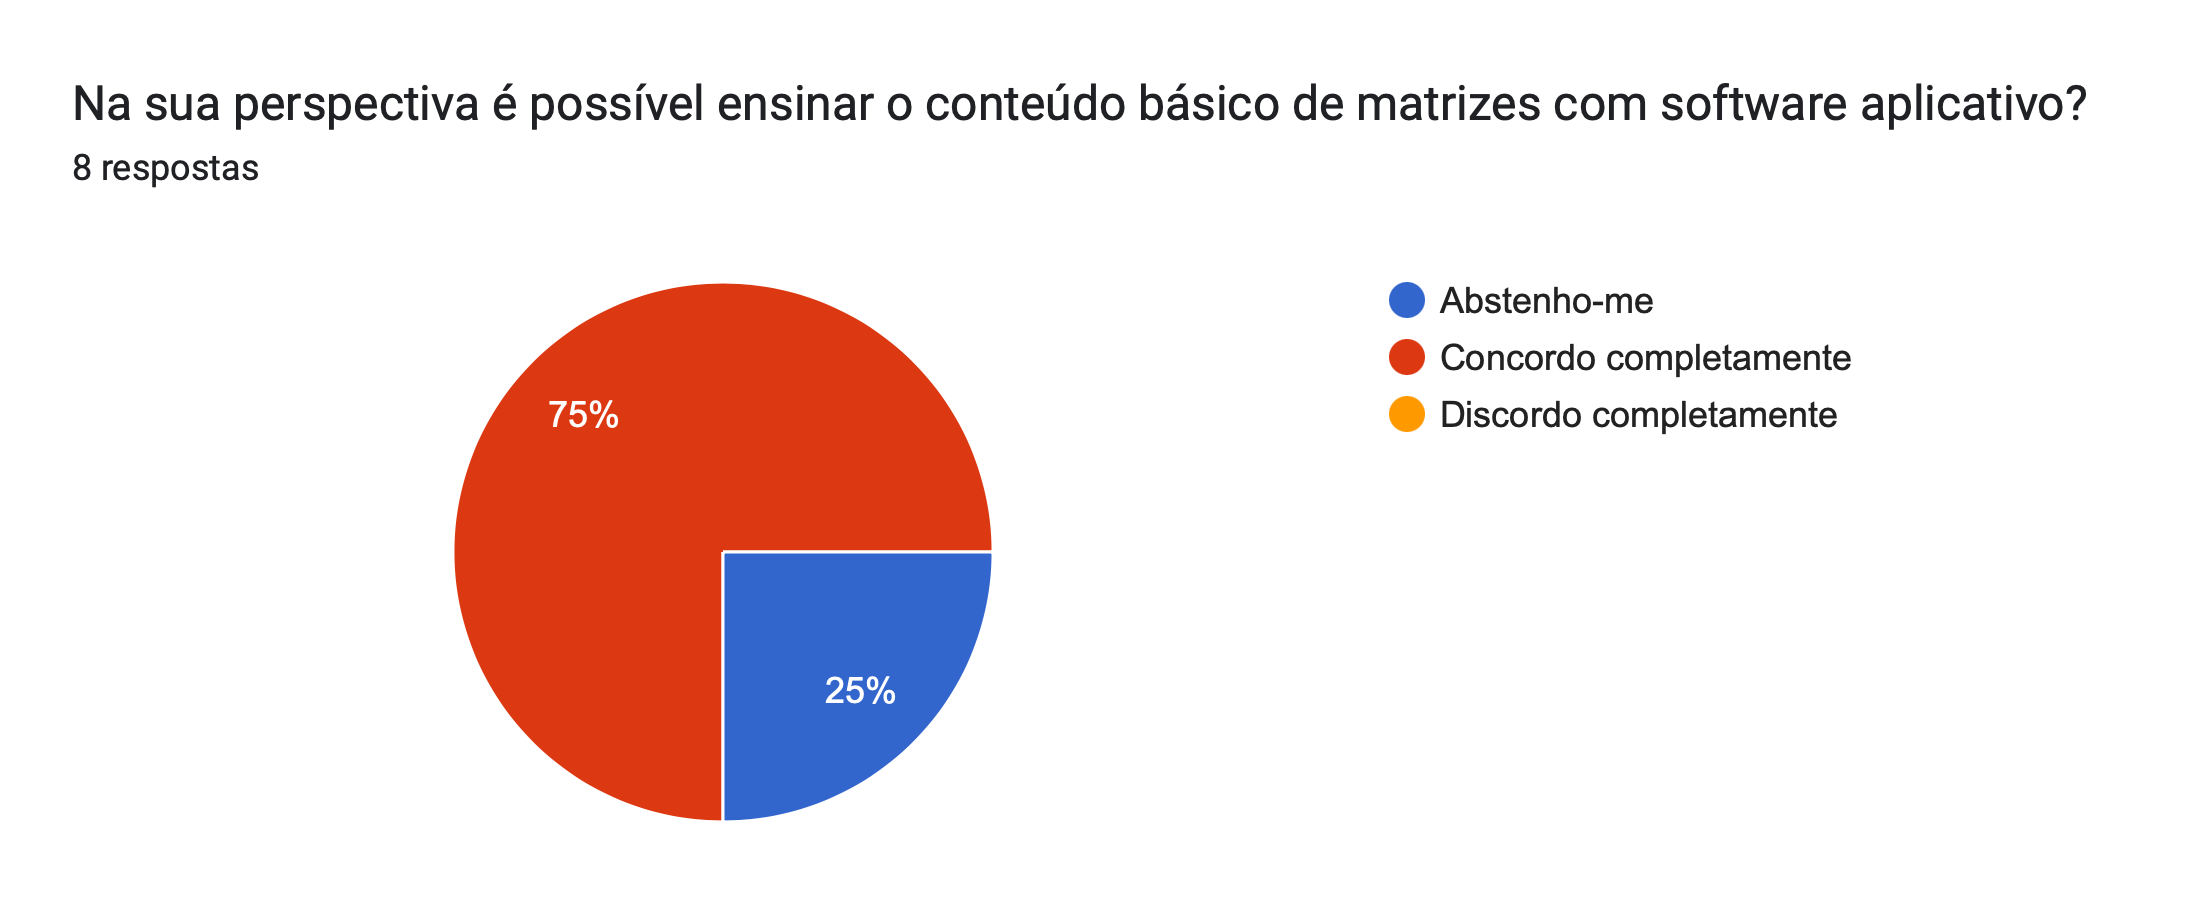
\includegraphics[scale=0.2]{figuras/resultados/ensino_matriz_app.png}
    \label{fig:ensino_matriz_app}
    \legend{Fonte: Eonay e Klenilmar (2024).}
\end{figure}


%De forma geral foi analisado a perspectiva dos docentes para uso de ferramentas diversas para o ensino não somente na matemática ou na área de exatas mas em um contexto maior, onde 12,5\% apontaram como regular ou muito satisfatório e 75,0\% como satisfatório.


De modo geral, foi analisada a perspectiva dos docentes quanto ao uso de ferramentas diversas no ensino não se limitando apenas à matemática ou às áreas de exatas, mas abrangendo um contexto mais amplo quantificado na Figura \ref{fig:soft_app_ensino}. Os resultados indicaram que 12,5\% dos participantes consideraram o uso dessas ferramentas como regular ou muito satisfatório, enquanto 75,0\% avaliaram como satisfatório. Esses dados refletem uma aceitação positiva, embora com margem para aprimoramento na integração dessas ferramentas no processo de ensino-aprendizagem.

\begin{figure}[h!]
    \caption{Uso geral de softwares/aplicativos no ensino}
    \centering
    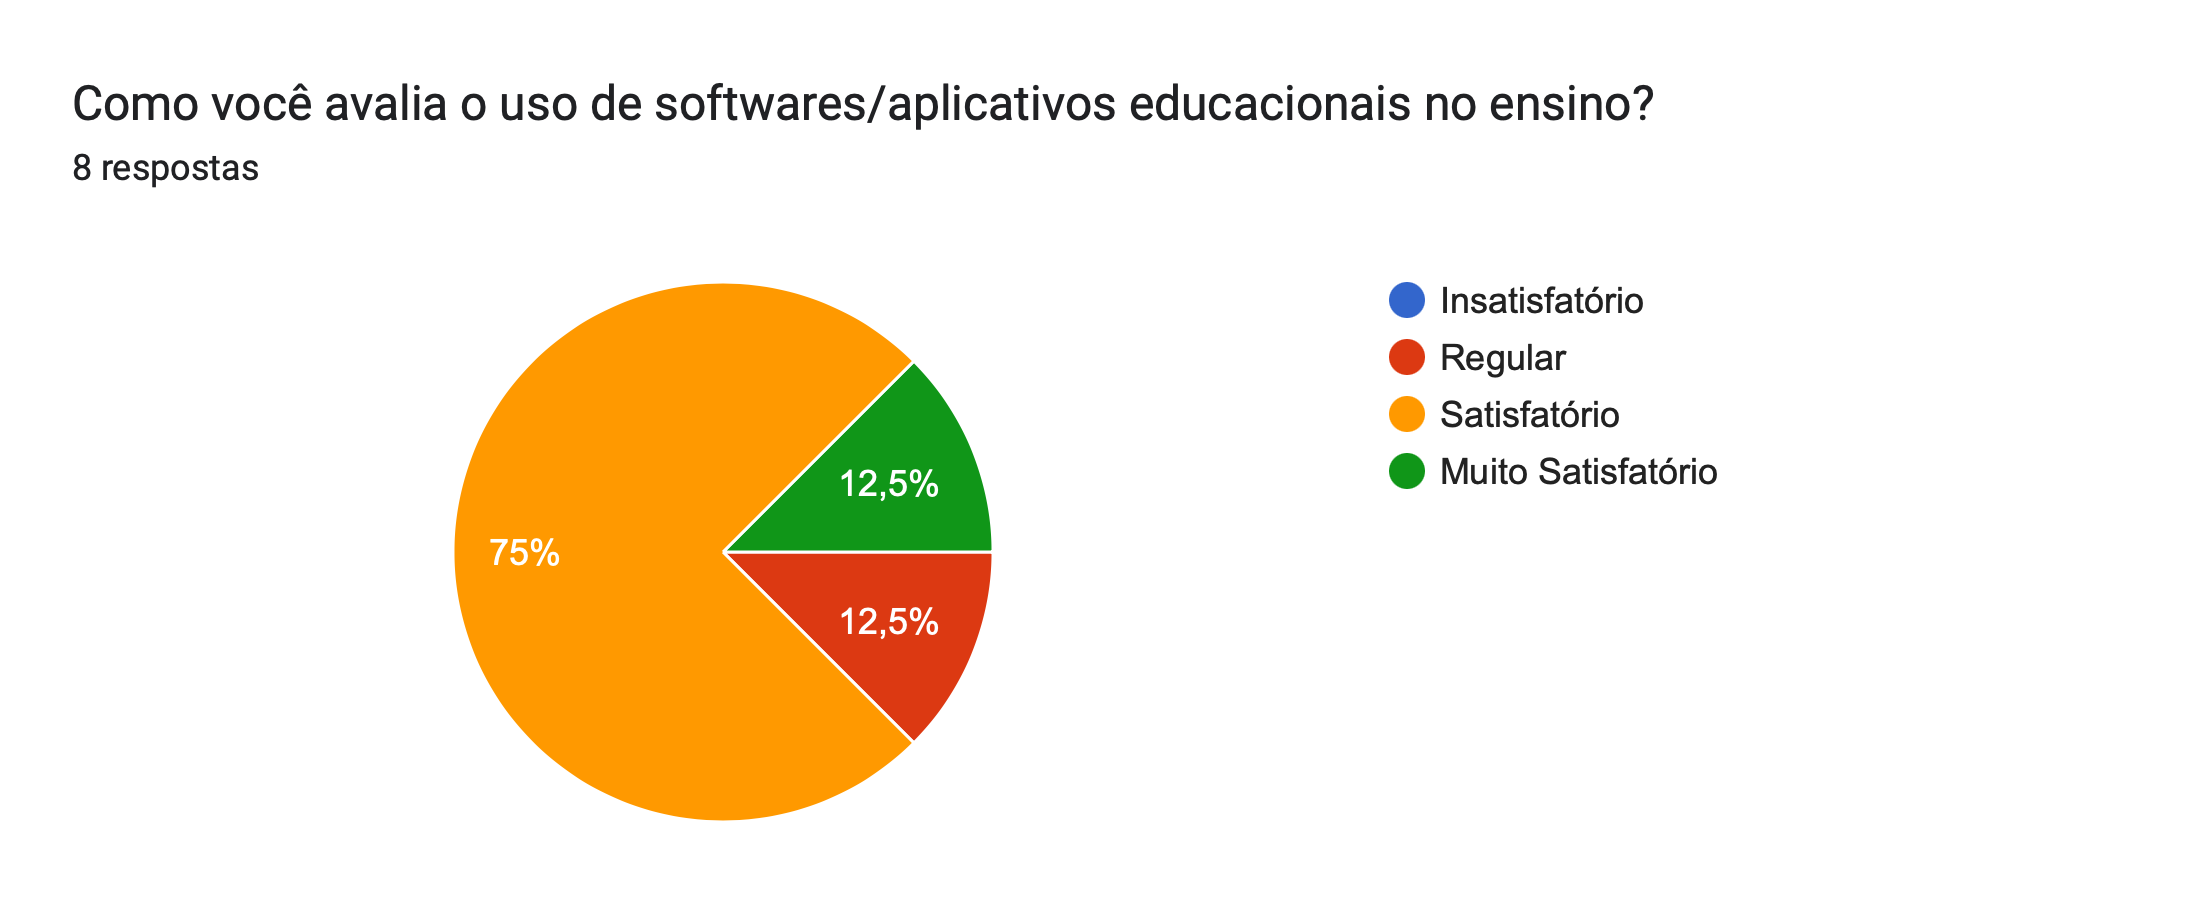
\includegraphics[scale=0.2]{figuras/resultados/app_ensino.png}
    \label{fig:soft_app_ensino}
    \legend{Fonte: Eonay e Klenilmar (2024).}
\end{figure}








\section{Produto Educacional}
\label{produto_educacional}

Disponibilização do produto educacional, software em formato REA (Recurso Educacional Aberto), tem objetivo de consolidação e aprimoramento pela comunidade acadêmica. O software foi desenvolvido no formato PWA é um acrônimo para \textit{Progressive Web Apps}, ou Aplicações Web Progressivas. A palavra \textit{progessiva} vem da ideia de \textit{Progressive Enhancement}, ou melhoria progressiva. Neste contexto, a ideia por trás da palavra \textit{progressiva} é condicionar uma aplicação a atender o maior número de pessoas possível, sob todos os aspectos \cite{pontes2018progressive}.


O formato PWA permite ampla compatibilidade com múltiplas plataformas, como Web, Android e iOS, e garante o funcionamento em diversos dispositivos, incluindo portáteis, como \textbf{tablets, smartphones e laptops}. Essa característica amplia o alcance e a acessibilidade da solução proposta.

O artefato, concebido como um Produto Educacional\footnote{http://eonay.ddns.net:8000}, publicado em repositório público, permitindo que outros docentes o utilizem em suas práticas pedagógicas. Dessa forma, ele pode ser aplicado em conjunto com diversas técnicas de ensino, tanto no ambiente educacional formal quanto no não formal, contribuindo para o desenvolvimento da aprendizagem dos educandos.

O Mathix é voltado para o currículo que aborda a componente de introdução a matrizes, utilizando uma aplicação em plataforma Web. A ferramenta promove uma abstração dos conceitos fundamentais de matrizes, estabelecendo uma relação prática entre teoria e aplicação. Ela é adaptável tanto para cursos presenciais quanto a distância, aproveitando a conectividade da rede mundial de computadores. É importante destacar que as características do produto foram definidas com base em um levantamento documental realizado durante a pesquisa, visando atender às demandas práticas da docência no processo de mediação do ensino-aprendizagem.

Com foco em auxiliar a prática docente, o produto educacional se distingui pela flexibilidade do software, podendo ser utilizado em ambientes formais e não formais de ensino. Além disso, ao seguir as orientações docentes de sustentação teórica, ele também pode ser empregado para estudos individuais. A ferramenta favorece ainda a integração com outras áreas de conhecimento, como estruturas de dados, programação, e mapeamento, sendo uma base útil para diversas aplicações e tarefas correlatas.


O produto também planeja-se a adaptação para uso do método de sala de aula invertida como objetivo contribuir e diversificar a adoção de tecnologias que podem agregar outros instrumentos para corroborar ou melhorar processo de ensino e aproximando mais o aluno do conteúdo. Para concepção do produto na perspectiva de \citeonline{kaplun2003material}, identificam-se três eixos correlacionados que se integram para o desenvolvimento de um Produto Educacional, segue: o eixo \textbf{conceitual}, o \textbf{pedagógico} e o \textbf{comunicacional}.


As três etapas paralelamente implementadas em quaisquer ferramenta proporcionam engajamento dos estudantes para alcançar o seu objetivo, neste sentido para \citeonline{kaplun2003material}, reforça o tripe conceitual, pedagógico e comunicacional para com  foco na metodologia aplicada no desenvolvimento na experiencia do usuário e na interface com usuário, deve-se também trabalhar em conjunto com outras práticas que remetam a um aprendizado significativo mediado por tecnologias.



A combinação dos eixos conceitual, pedagógico e comunicacional é essencial para criar uma \textbf{experiência de aprendizagem} eficaz e envolvente guiada pelo docente. O eixo conceitual estabelece os fundamentos teóricos, o pedagógico propõe as abordagens e estratégias de ensino, e o comunicacional garante que a interação entre o aluno e o conteúdo seja clara e envolvente.

Esses eixos interagem para fornecer uma abordagem holística, onde o aluno não só tem acesso ao conteúdo, mas é incentivado a se engajar ativamente com ele. No contexto da sala de aula invertida, isso se traduz em uma experiência onde o aluno assume maior responsabilidade por seu próprio aprendizado, com o apoio de ferramentas tecnológicas que potencializam o processo. A experiência do usuário e a interface com o aluno devem ser desenhadas de forma a facilitar esse engajamento, garantindo que a tecnologia seja um meio para um aprendizado significativo e não um fim em si mesma. Portanto, a colaboração entre esses três eixos é fundamental para o sucesso do produto educacional e para o desenvolvimento de uma aprendizagem mais rica e dinâmica.






Para desenvolvimento da proposta do produto alguns instrumentos foram utilizados, a princípio todas as ferramentas baseadas em \textbf{software livre}, segue: linguagem de programação Python, biblioteca Numpy para manipulação de vetores, framework para aplicações web Django e dentre outras para aplicações das regras de negócio conceituais aplicadas de forma pedagógica com uma interface acessível, segue a interface principal na Figura \ref{fig:home_mathix}:

\begin{figure}[h!]
    \caption{Interface principal Mathix}
    \centering
    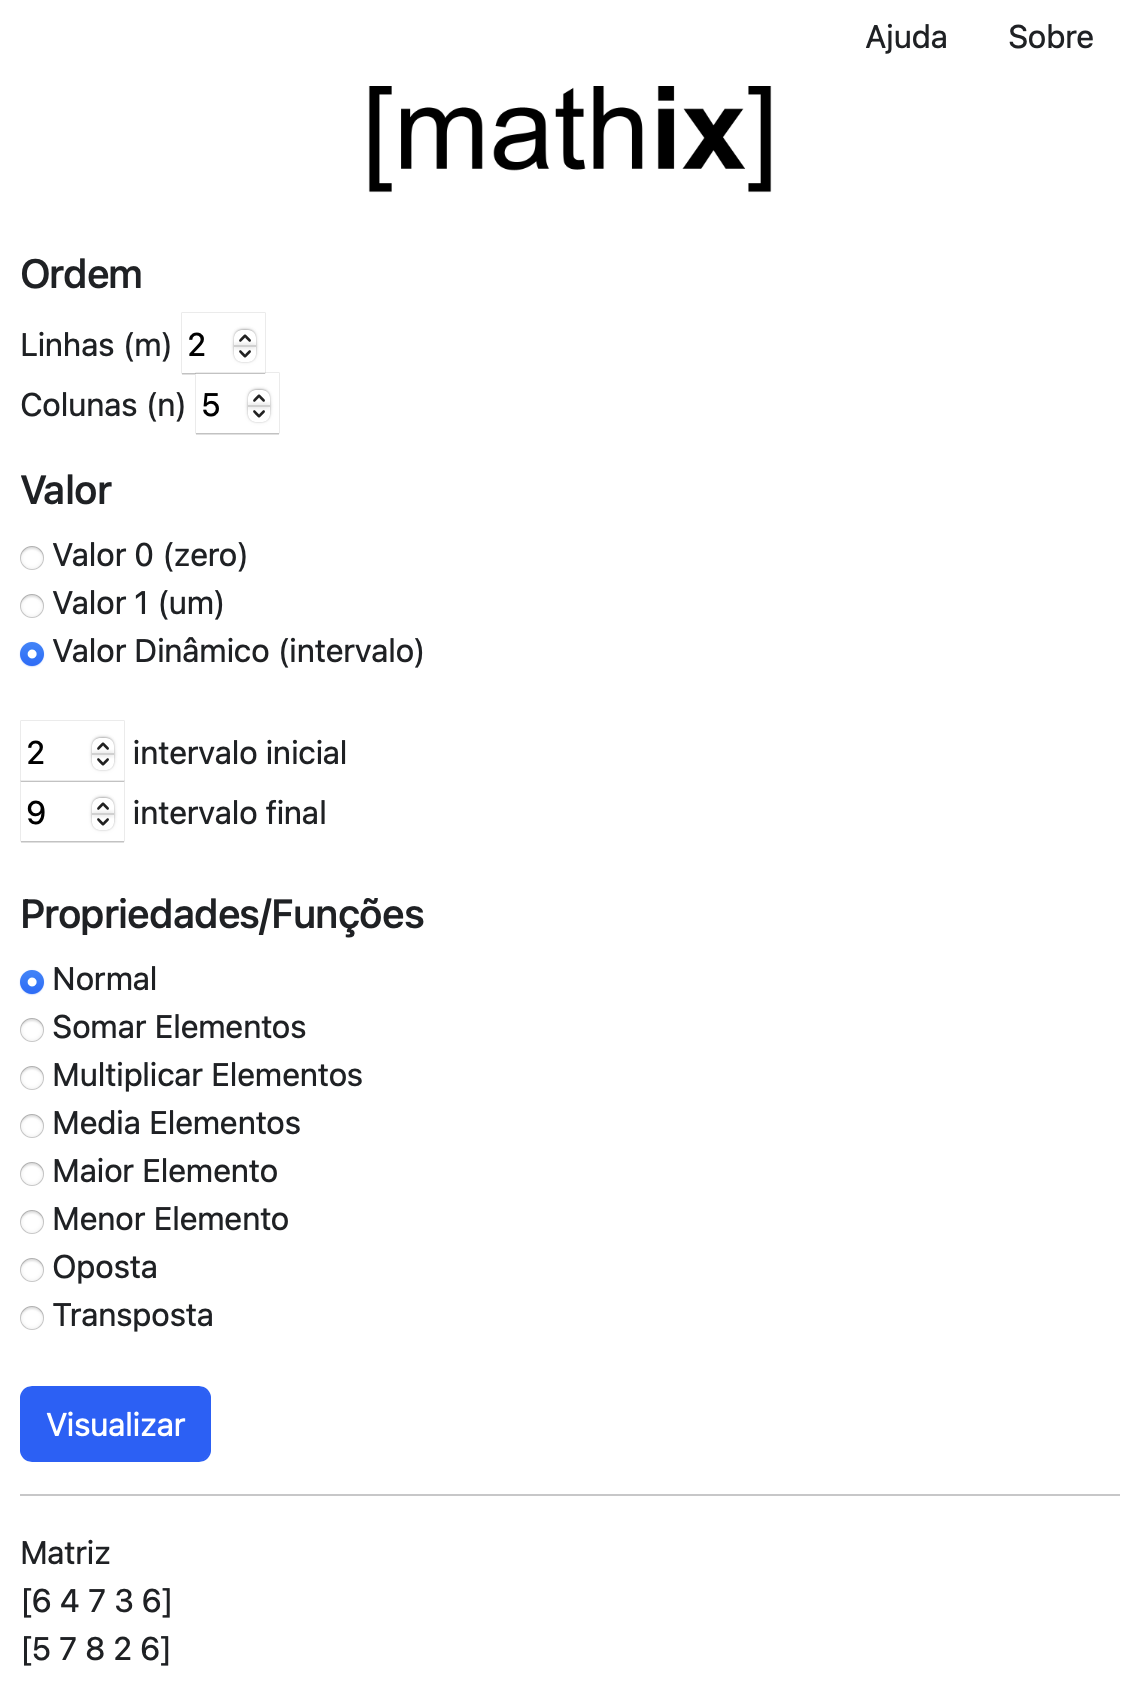
\includegraphics[scale=0.4]{figuras/mathix-home.png}
    \label{fig:home_mathix}
    \legend{Fonte: Eonay e Klenilmar (2024).}
\end{figure}

Se propôs o nome para a ferramenta de \textbf{Mathix} em referencia a palavra matriz e matemática com um arranjo em conjunto a outra referência ao número 9 (nove) representado algarismo romano, segue na Figura \ref{fig:logo_mathix} a proposição de logo.

\begin{figure}[h!]
    \caption{Logomarca Mathix}
    \centering
    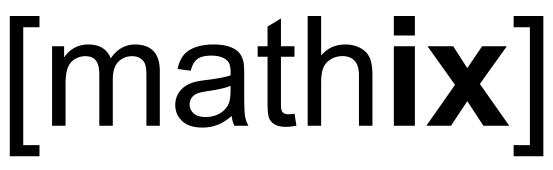
\includegraphics[scale=0.4]{figuras/mathix_logo.png}
    \label{fig:logo_mathix}
    \legend{Fonte: Eonay e Klenilmar (2024).}
\end{figure}

Outro ponto a ressaltar é que este trabalho contou com a colaboração do \textbf{GPTICAM} (Grupo de Pesquisa em Tecnologias da Informação e Comunicação na Amazônia) onde dentre as linhas de pesquisa a Engenharia de Software corroborar com o desenvolvimento do produto educacional. Ressaltar que durante o andamento dos trabalhos outras atividades ou produtos podem ser derivados da pesquisa assim como a inclusão de novos recursos ao Mathix.


O objeto educacional final será um Recurso Educacional Aberto (REA) que assegura a utilização, modificação e reutilização do produto para futuras pesquisas na área da educação e consequentemente sua evolução, melhorias e agregação para novas versões ou aplicação em conjunto com novos projetos. O conceito de REA segundo \cite{nobre2016incorporar}:


\begin{citacao}
Os materiais de ensino, aprendizagem e investigação em quaisquer suportes, digitais ou outros, que se situem no domínio público ou que tenham sido divulgados sob licença aberta que permite acesso, uso, adaptação e redistribuição gratuitos por terceiros, mediante nenhuma restrição ou poucas restrições. O licenciamento aberto é construído no âmbito da estrutura existente dos direitos de propriedade intelectual, tais como se encontram definidos por convenções internacionais pertinentes, e respeita a autoria da obra \cite{nobre2016incorporar}.
\end{citacao}

Contudo o resultado visa contribuir para prática docente tornando-a mais atrativa aos educandos, podendo ser empregado em múltiplas áreas que se utilizam do conceito de matrizes, pelas características pode ser agregada em outras plataformas como AVA (Ambiente Virtual de Aprendizagem) entre outras para fortalecimento do ensino.




\section{Avaliação do Produto Educacional}
\label{avaliacao_pe}

Após a disponibilização do produto educacional Mathix para uso e testes, recebemos diversos \textit{feedbacks} de profissionais da área educacional, os quais avaliaram a ferramenta e a sua aplicabilidade no ensino, considerando seu modelo de Produto Mínimo Viável (PMV). A seguir, apresentamos os resultados obtidos a partir da aplicação de um questionário sobre o uso da ferramenta no ensino, conforme mostrado na Tabela \ref{tab:p1}.


%%% Pergunta 01

\begin{table}[h!]
    \centering
    \caption{O produto educacional deve ser utilizado no ensino}
    \begin{tabular}{c|c|c}
        \textbf{Resposta} &	\textbf{Absoluto} & \textbf{Relativo} \\
        \hline
        Sim & 7 & 87,5\% \\
        \hline
        Não & 1 & 12,5\% \\
    \end{tabular}
    \legend{Fonte: Eonay e Klenilmar (2024).}
    \label{tab:p1}
\end{table}


De acordo com os dados da Tabela \ref{tab:p1}, aproximadamente 87,5\% dos participantes acreditam que a ferramenta deve ser utilizada no ensino, enquanto 12,5\% são contrários ao seu uso no contexto educacional. Além disso, a questão sobre a aderência do produto à prática docente também foi analisada. Considerando aspectos como confiabilidade e facilidade de uso, já que se tratava do primeiro contato dos participantes com a ferramenta, os resultados indicaram que 87,5\% utilizariam a ferramenta em suas aulas, enquanto 12,5\% não optariam por usá-la, como representado na Figura \ref{fig:p2}


%%% Pergunta 02
\begin{figure}[h!]
    \caption{Utilizaria o PE em sua prática docente}
    \centering
    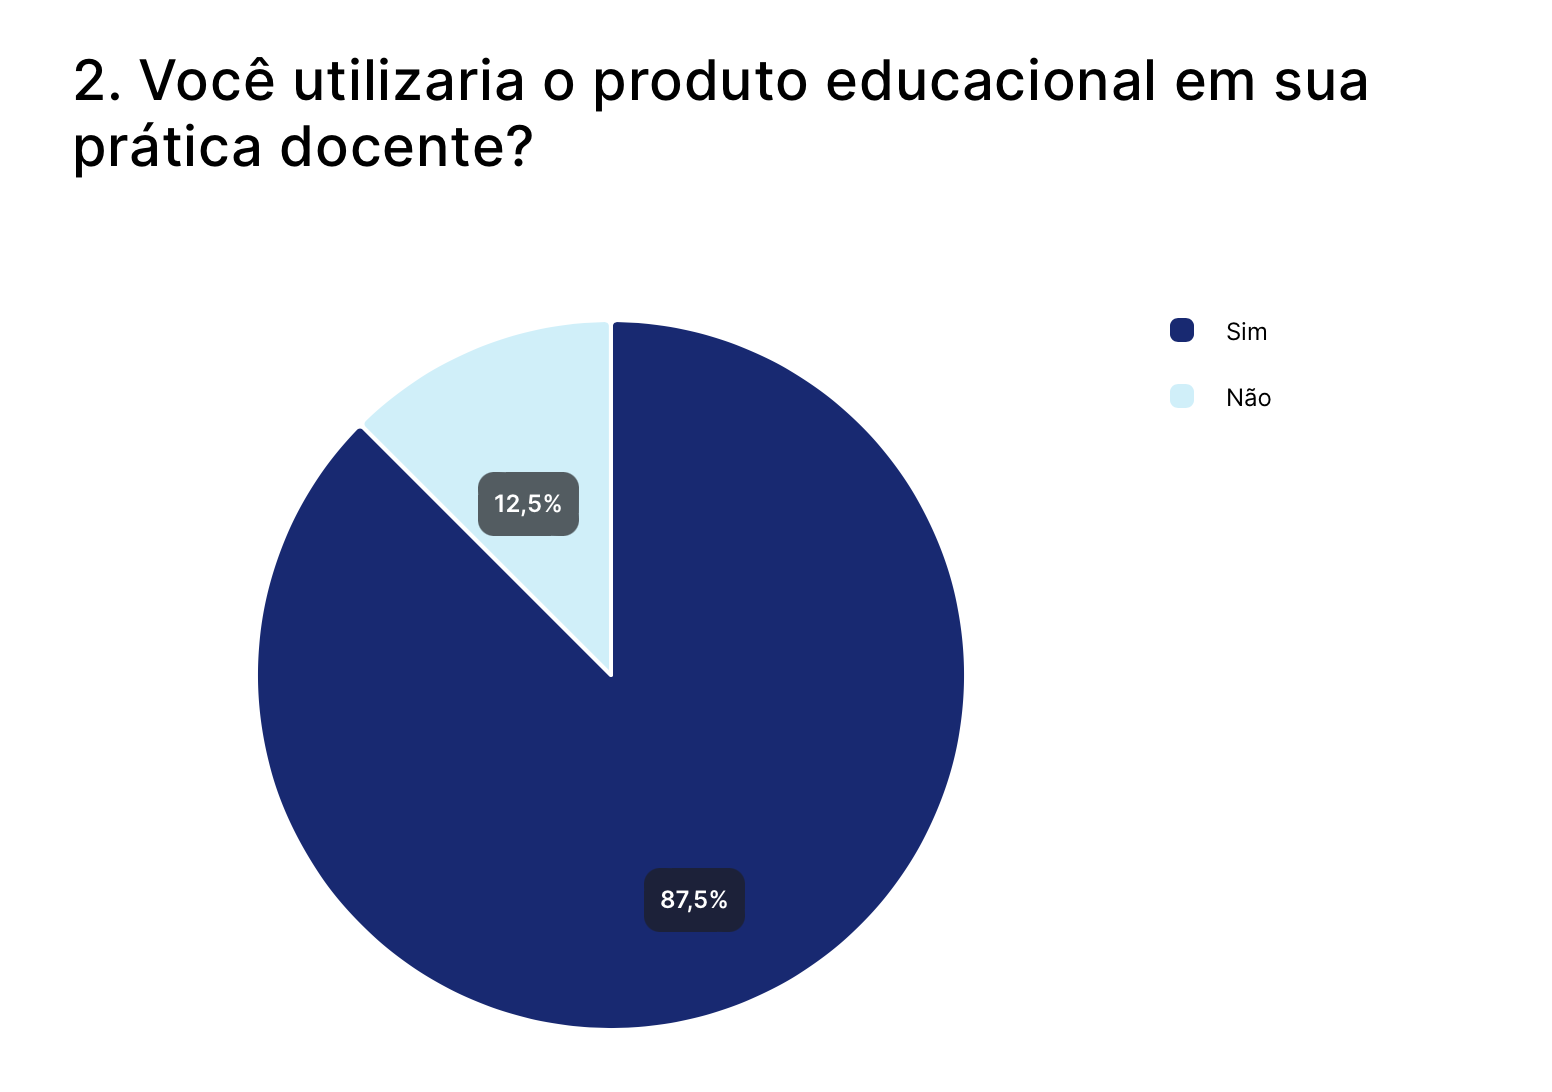
\includegraphics[scale=0.3]{figuras/resultados/p2.png}
    \label{fig:p2}
    \legend{Fonte: Eonay e Klenilmar (2024).}
\end{figure}




%%% Pergunta 03
Outro ponto relevante foi a avaliação da satisfação dos participantes em relação ao uso do produto educacional, que foi disponibilizado na forma de software/aplicativo. Vale destacar que todos os participantes utilizaram a plataforma de maneira independente, sem restrições e, em alguns casos, de forma concorrente com outras ferramentas. Os resultados, apresentados na Tabela \ref{tab:p3}, mostram que 62,5\% consideraram o produto Satisfatório, 25,0\% o avaliaram como Muito Satisfatório e 12,5\% o classificaram como Regular em relação à satisfação com o uso da ferramenta.


\begin{table}[h!]
    \centering
    \caption{Surgiu alguma dificuldade em manusear o produto educacional}
    \begin{tabular}{c|c|c}
        \textbf{Resposta} &	\textbf{Absoluto} & \textbf{Relativo} \\
        \hline
        Sim & 6 & 75,0\% \\
        \hline
        Não & 2 & 25,0\% \\
    \end{tabular}
    \legend{Fonte: Eonay e Klenilmar (2024).}
    \label{tab:p3}
\end{table}



%%% Pergunta 04

A seguir, foi investigada a dificuldade de manuseio da plataforma, levando em conta seu formato livre, interface clean (limpa) e a ausência de manuais de instrução. A Tabela \ref{tab:p3} resume os indicadores de dificuldade relacionados a essa questão. Vale ressaltar que uma características de plataforma é a questão da usabilidade, configurabilidade, extensibilidade e instalabilidade.


A satisfação de utilizar o software representado na Tabela \ref{tab:p4}, em utiliza-ló sem a necessidade de manuais está diretamente ligada à sua interface intuitiva e à experiência fluida que oferece. Quando se trata de um Produto Mínimo Viável (PMV), a simplicidade e funcionalidade se destacam, tornando o uso natural e acessível, mesmo sem um guia extenso. Para plataformas educacionais que abstraem teorias complexas, o software se torna uma ferramenta poderosa ao transformar conceitos abstratos em experiências práticas e compreensíveis. Isso permite que os usuários, sejam alunos ou educadores, interajam de forma eficaz com o conteúdo, sem sobrecarga cognitiva, promovendo um aprendizado mais envolvente e eficiente.


\begin{table}[h!]
    \centering
    \caption{De forma geral, sua satisfação ao utilizar o produto educacional na forma software/aplicativo}
    \begin{tabular}{c|c|c}
        \textbf{Resposta} &	\textbf{Absoluto} & \textbf{Relativo} \\
        \hline
        Satisfatório & 5 & 62,5\% \\
        \hline
        Muito Satisfatório & 2 & 25,0\% \\
        \hline
        Regular & 1 & 12,25\% \\
        \hline
        Insatisfatório & 0 & 0,0\% \\
    \end{tabular}
    \legend{Fonte: Eonay e Klenilmar (2024).}
    \label{tab:p4}
\end{table}


%%% Pergunta 05

O produto educacional Mathix tem como objetivo auxiliar a prática docente, especialmente no ensino de matrizes, oferecendo uma plataforma rápida e flexível. Perguntou-se aos participantes se o produto correspondeu às expectativas relacionadas ao seu propósito, e os resultados estão apresentados na Tabela \ref{tab:p5}. Dentre os participantes, 62,5\% consideraram o produto Satisfatório em termos de seu propósito, 12,5\% o avaliaram como Muito Satisfatório, enquanto 12,5\% classificaram-no como Regular, evidenciando que a ferramenta ainda se encontra em sua fase inicial e possui funcionalidades limitadas.


\begin{table}[h!]
    \centering
    \caption{A aplicação propôs a fazer a função para qual foi desenvolvido}
    \begin{tabular}{c|c|c}
        \textbf{Resposta} &	\textbf{Absoluto} & \textbf{Relativo} \\
        \hline
        Satisfatório & 6 & 62,5\% \\
        \hline
        Muito Satisfatório & 1 & 12,5\% \\
        \hline
        Regular & 1 & 12,25\% \\
        \hline
        Insatisfatório & 0 & 0,0\% \\
    \end{tabular}
    \legend{Fonte: Eonay e Klenilmar (2024).}
    \label{tab:p5}
\end{table}



%%% Pergunta 06

Por fim, de forma opcional, foi solicitado aos participantes que dessem sugestões de melhorias para o produto educacional, com base em suas experiências. Quatro relatos construtivos foram obtidos, abordando aspectos relacionados à Experiência do Usuário (UX) e à Interface do Usuário (UI), os quais foram considerados importantes para aprimorar a usabilidade e a efetividade do produto.


\begin{citacao}

    \item "Parabéns pela iniciativa, inserir outras tarefas que se utiliza matrizes";

    \item "Os resultados poderiam ficar ao lado em vez de baixo por conta do local de exibição na tela";

    \item "Inicialmente não deve-se utilizar para não produzir efeito de facilidade, mas pode ser utilizado para atividades";

    \item "Em uma perspectiva geral eu achei que o Mathix tem uma estética simples e clara, e fácil de usar. Mas pensando em um usuário em nível inicial, deixar visíveis os rótulos dos campos na tela facilitariam o uso (os mesmos do menu Ajuda). Nos resultados disponibilizar uma curta explicação das Propriedades. E caso o usuário deixe os campos linhas e colunas vazios, informar que os campos precisam ser preenchidos";

\end{citacao}







\subsection{Avaliação de Interface de Usuário (UI)}
\label{avaliacao_ui}

Em conjunto a avaliação do PE foi analisado a interface para com características que variam em percentuais fixos que varias a cada 20\% para cada opção de resposta, inicialmente foi questionado a possibilidade de recomendação a seus pares (outros docentes), Tabela \ref{tab:ui-1} segue: 

\begin{table}[h!]
    \centering
    \caption{Qual é a probabilidade de você recomendar o Mathix para outros docentes}
    \begin{tabular}{c|c|c}
        \textbf{Resposta} &	\textbf{Absoluto} & \textbf{Relativo} \\
        \hline
        Muito alto 75\% & 5 & 62,5\% \\
        \hline
        Extremamente alto 100\% & 2 & 25,0\% \\
        \hline
        Talvez sim, talvez não 50\% & 1 & 12,5\% \\
        \hline
        Baixo 25\% & 0 & 0,0\% \\
        \hline
        Nenhuma 0\% & 0 & 0,0\% \\
    \end{tabular}
    \legend{Fonte: Eonay e Klenilmar (2024).}
    \label{tab:ui-1}
\end{table}

Obtivemos cerca de 62,5\% dos participantes que recomendariam a outros colegas docentes com intensidade de muito alta e 25\% optaram por recomendar de forma extremamente alta, seguido de 12,5\% que têm duvidas sobre a recomendação. Consequentemente recomenda-se algo que desperte interesse e que seja performático na perspectiva do usuário, na Tabela \ref{tab:ui-2} foi analisado a questão do desempenho.


\begin{table}[h!]
    \centering
    \caption{Qual é a sua opinião geral sobre o desempenho do Mathix}
    \begin{tabular}{c|c|c}
        \textbf{Resposta} &	\textbf{Absoluto} & \textbf{Relativo} \\
        \hline
        Bom & 4 & 50,0\% \\
        \hline
        Ótimo & 3 & 37,5\% \\
        \hline
        Regular & 1 & 12,5\% \\
        \hline
        Ruim & 0 & 0,0\% \\
        \hline
        Péssimo & 0 & 0,0\% \\
    \end{tabular}
    \legend{Fonte: Eonay e Klenilmar (2024).}
    \label{tab:ui-2}
\end{table}

No contexto do desempenho em plataformas web, é essencial destacar a relevância desse aspecto para a experiência do usuário. A velocidade e a eficiência de um site ou aplicação têm impacto direto na usabilidade e na satisfação dos usuários. Estudos indicam que a otimização do desempenho não apenas melhora a experiência do usuário, mas também influencia fatores cruciais como taxas de conversão, retenção e satisfação geral.

De acordo com uma pesquisa da Google, um atraso de apenas um segundo no tempo de carregamento de uma página pode reduzir as conversões em até 20\% \cite{google2018speed}. Esses dados reforçam a importância de priorizar melhorias de performance como parte das estratégias de desenvolvimento e manutenção de plataformas digitais. Outro aspecto analisado é com relação a travamentos e falhas mostrado na Tabela \ref{tab:ui-3}:



\begin{table}[h!]
    \centering
    \caption{Com que frequência o Mathix costuma congelar ou falhar}
    \begin{tabular}{c|c|c}
        \textbf{Resposta} &	\textbf{Absoluto} & \textbf{Relativo} \\
        \hline
        Ainda não sei & 5 & 62,5\% \\
        \hline
        Nunca & 2 & 25,0\% \\
        \hline
        Ocasionalmente & 1 & 12,5\% \\
        \hline
        Frequentemente & 0 & 0,0\% \\
        \hline
        Constantemente & 0 & 0,0\% \\
    \end{tabular}
    \legend{Fonte: Eonay e Klenilmar (2024).}
    \label{tab:ui-3}
\end{table}

O dados corroboram com a avaliação de desempenho e revelam que 62,5\% durante o uso optaram por "Ainda não sei", e 25,0\% como "Nunca" o que leva a concluir sobre a estabilidade do software, também responderam com 12,5\% como ocasionalmente obtiveram alguma instabilidade durante os testes.

Se tratando do uso, a investigação computou a informação sobre a facilidade baseada na interface e interatividade do participante Tabela \ref{tab:ui-4}, onde 50\% dos participantes afirmaram ser extremamente fácil e 37,5\% como muito fácil, afirmando simplicidade da ferramenta, ainda 12,5\% acreditam não ser muito fácil utilizar.


\begin{table}[h!]
    \centering
    \caption{Quão fácil de ser usada é a interface do Mathix}
    \begin{tabular}{c|c|c}
        \textbf{Resposta} &	\textbf{Absoluto} & \textbf{Relativo} \\
        \hline
        Extremamente fácil & 4 & 50,0\% \\
        \hline
        Muito fácil & 3 & 37,5\% \\
        \hline
        Não muito fácil & 1 & 12,5\% \\
        \hline
        Moderadamente fácil & 0 & 0,0\% \\
        \hline
        Nada fácil & 0 & 0,0\% \\
    \end{tabular}
    \legend{Fonte: Eonay e Klenilmar (2024).}
    \label{tab:ui-4}
\end{table}

Uma das dificuldade que os usuários enfrentam é com relação aos requisitos e instalação de ferramenta para utilização, assim a Tabela \ref{tab:ui-5} traz 87,5\% informando facilidade extrema e de formada moderada 12,5\% em instalar e configurar o PE para operação.

\begin{table}[h!]
    \centering
    \caption{Quão fácil foi instalar o nosso Mathix}
    \begin{tabular}{c|c|c}
        \textbf{Resposta} &	\textbf{Absoluto} & \textbf{Relativo} \\
        \hline
        Extremamente fácil & 7 & 87,5\% \\
        \hline
        Moderadamente fácil & 1 & 12,5\% \\
        \hline
        Nada fácil & 0 & 0,0\% \\
    \end{tabular}
    \legend{Fonte: Eonay e Klenilmar (2024).}
    \label{tab:ui-5}
\end{table}

De forma optativa foi perguntado quais aspectos do Mathix precisamos melhorar e de forma a correlacionar e categorizar os \textit{feedback} das respostas:

\begin{citacao}
    \item "Uma interface um pouco mais intuitiva no processo construtivo das matrizes, considerando os valores específicos dos termos e uma melhor visualização gráfica, porém é satisfatório considerando as propostas de operações". \textbf{Categoria}: Interface.
    
    \item "Tutorial sobre o uso do Mathix". \textbf{Categoria}: Manual.
    
    \item "Possibilidade de impressão de tarefas e inserir outras funções para com as matrizes". Categoria: Interface e Funcionalidade.
    
    \item "Gostaria que o Mathix além de mostrar o resultado final, mostrasse o passo a passo daquele resultado. Senti falta da matriz inversa" . \textbf{Categoria}: Interface e Funcionalidade.
    
    \item "Como o foco do Mathix é abordar matrizes em um nível introdutório, considero que para iniciantes alguns esclarecimentos poderiam ficar fixados na interface (para facilitar o uso). Por exemplo: Valor Dinâmico (intervalo): Especifique um valor (aceita valores positivos e negativos). Seria interessante exibir uma explicação curta no resultado, para ajudar o estudante no aprendizado. Por exemplo, Matriz oposta (Para os elementos correspondentes inverte-se o sinal do valor)". \textbf{Categoria}: Interface e Manual.
    
    \item "Adicionar outras operações com matrizes". \textbf{Categoria}: Funcionalidade.
\end{citacao}


Estas categorias percorridas trazem um indicador evolutivo do ponto de partida do produto educacional de \textbf{Interface, Manual e Funcionalidade} que podem e devem ser trabalhadas futuramente em outras versões. Por fim foi solicitado aos participantes um parecer final de avaliação da interface de forma optativa, segue:

\begin{citacao}

\item "Utilizaria como ferramenta complementar e não como ferramenta principal pois apenas mostra o resultado e falta de um viés didático. Por exemplo, muita vezes sem o auxilio do professor, o aluno o utilizaria para verificar algumas soluções. Mas o porque? Para que? ainda estão indefinidos. Gostei da iniciativa, mas o produto sem mostrar o passo a passo da solução e sem mostrar a matriz inversa, fica incompleto. Outra coisa, os elementos são apenas com valores inteiros";

\item "Simples, possibilita gerar item para exercícios";

\item "É um ferramenta que pode ser aplicadas para o aluno exercitar em casa e para uso no projetor para as aulas presenciais ou EAD";

\item "Considerando as propriedades propostas, seria altamente benéfico incluir a demonstração de outras operações e propriedades fundamentais que os alunos encontram ao ter o primeiro contato com o conteúdo de matrizes. Isso tornaria a experiência com o produto mais rica e envolvente, facilitando uma compreensão mais abrangente e prática do tema";

\item "Achei a ferramenta fácil de usar, tem uma estética simples e minimalista, incorpora um conjunto significativo de propriedades/funções de matrizes".

\end{citacao}

De forma geral a avaliação de 1 a 10 para a interface do produto educacional na Figura \ref{fig:ui-8}, representado na escala radial que demonstra um alto índice de satisfação no intervalo entre 6 e 9 como resultado indicador de aceitação pelos participantes.

\begin{figure}[h!]
    \caption{Grau de Satisfação do PE (UI)}
    \centering
    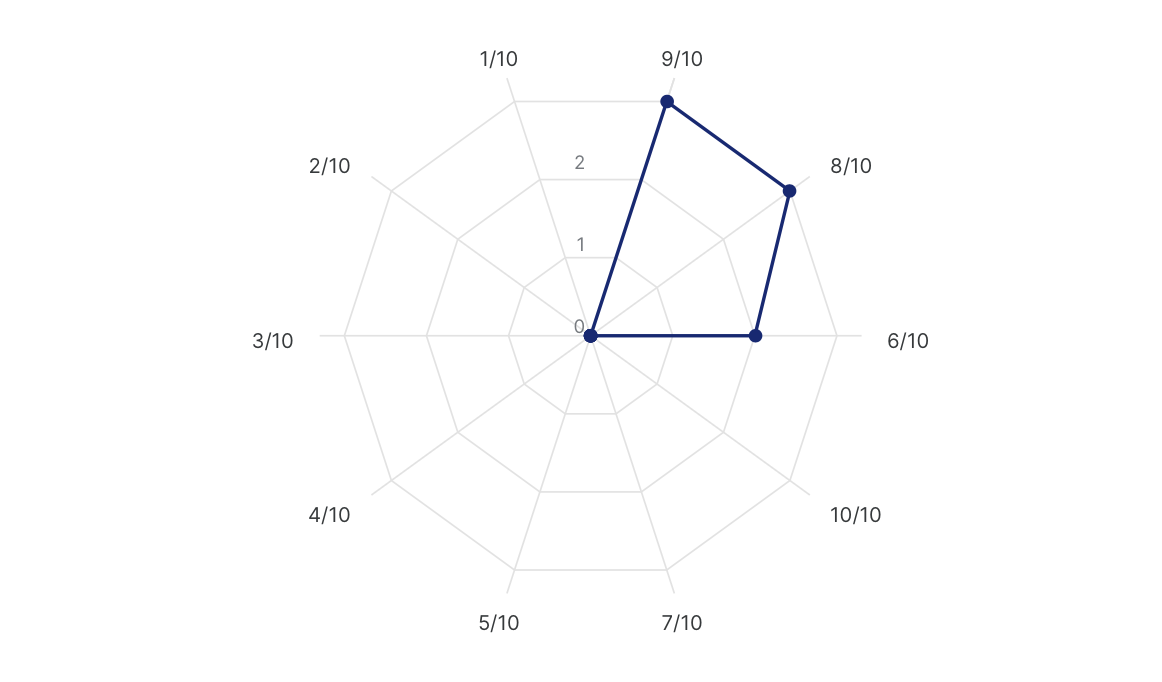
\includegraphics[scale=0.5]{figuras/resultados/satisfacao_ui.png}
    \label{fig:ui-8}
    \legend{Fonte: Eonay e Klenilmar (2024).}
\end{figure}











\subsection{Avaliação de Experiência de Usuário (UX)}
\label{avaliacao_ux}


Também em conjunto com a avaliação do PE foi analisado a experiencia do usuário para com características como \textbf{atratividade, controle, eficiência, estimulação, novidade e perspicuidade} para certos itens de cada respectivo grupo, cada opção de resposta variando entre -5 e 5 sendo, menor satisfação para maior satisfação respectivamente.

A Tabela \ref{fig:ux-1} retrata a avaliação de atratividade onde na visão dos participantes o produto educacional se mostrou agradável, atraente, atrativo e bom na avaliação media dos participantes. Para \citeonline{Tractinsky2000} "A atratividade de software está relacionada à combinação de estética, usabilidade e funcionalidade, sendo um fator crítico para a aceitação e retenção de usuários".

\begin{figure}[h!]
    \caption{Você gostou do produto}
    \centering
    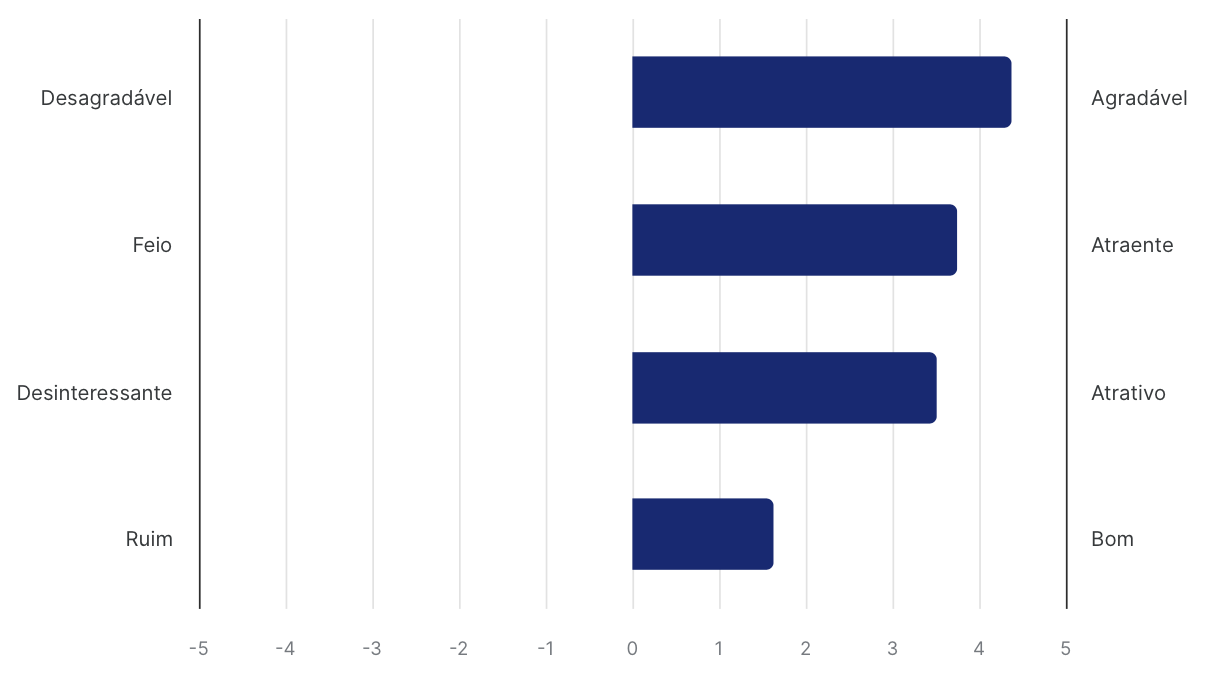
\includegraphics[scale=0.4]{figuras/resultados/ux-1.png}
    \label{fig:ux-1}
    \legend{Fonte: Eonay e Klenilmar (2024).}
\end{figure}

Alguns comentários deixados sobre atratividade apos a avaliação dos participantes:

\begin{citacao}
\item "Poderia ter um aplicativo específico";
\item "Funciona no celular e tablet de forma igual";
\item "Estudantes gostam quando professores saem do modelo convencional (aula explicativa e exercícios em papel). Então, a ferramenta é atrativa e interessante para estudantes aprender praticando".
\end{citacao}

Na Figura \ref{fig:ux-3} a avaliação de controle sobre o produto educacional eleva as características que atende a necessidade de forma segura.

\begin{figure}[h!]
    \caption{Você se sente no controle da situação durante a interação}
    \centering
    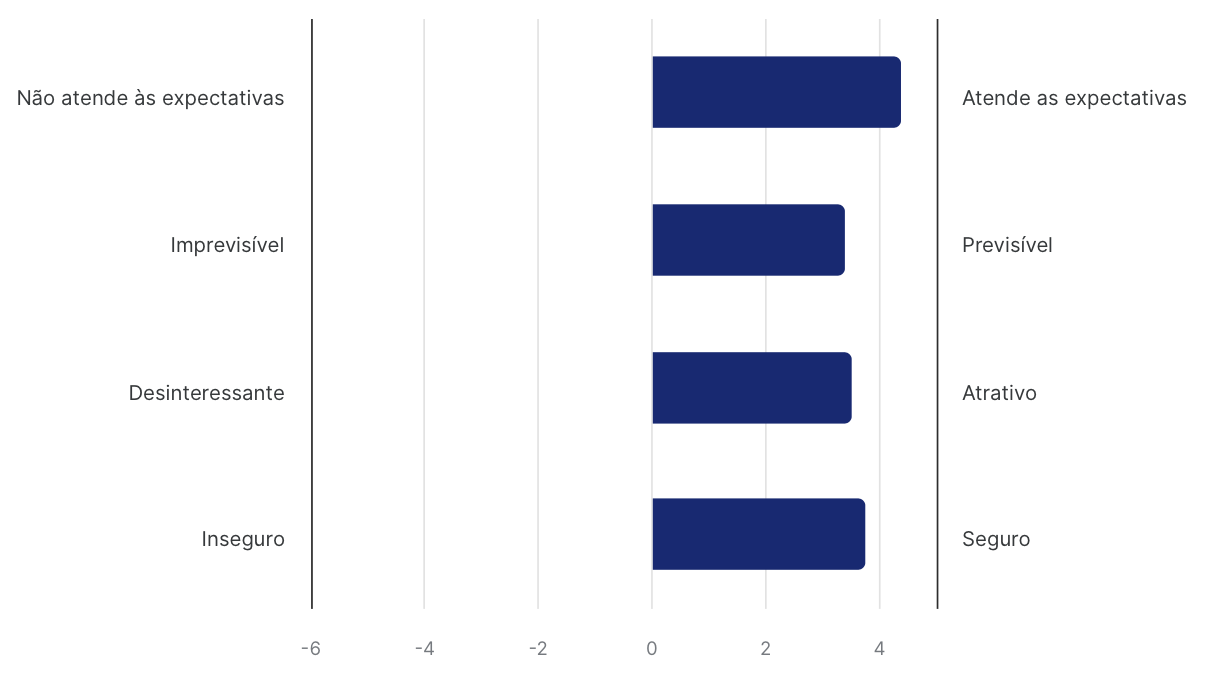
\includegraphics[scale=0.4]{figuras/resultados/ux-3.png}
    \label{fig:ux-3}
    \legend{Fonte: Eonay e Klenilmar (2024).}
\end{figure}

Um dos participantes deixou um comentário sobre o controle na avaliação:
"Lembrando que existem outras caracteristicas de matrizes que o sisteminha não contempla"\footnote{O texto encontra-se fidedigno ao texto coletado, caracteristicas entenda como características, sisteminha entenda como sistema ou produto educacional}. Reforço que o MPV é uma proposta inicial e deve ser continuado em trabalhos futuros pela comunidade. A avaliação do ponto de vista de eficiência também aponta na Figura \ref{fig:ux-5} indicativo de praticidade e rapidez que corrobora com a avaliação de desempenho da analise de interface.

\begin{figure}[h!]
    \caption{O produto pode ser utilizado de maneira fácil e eficiente}
    \centering
    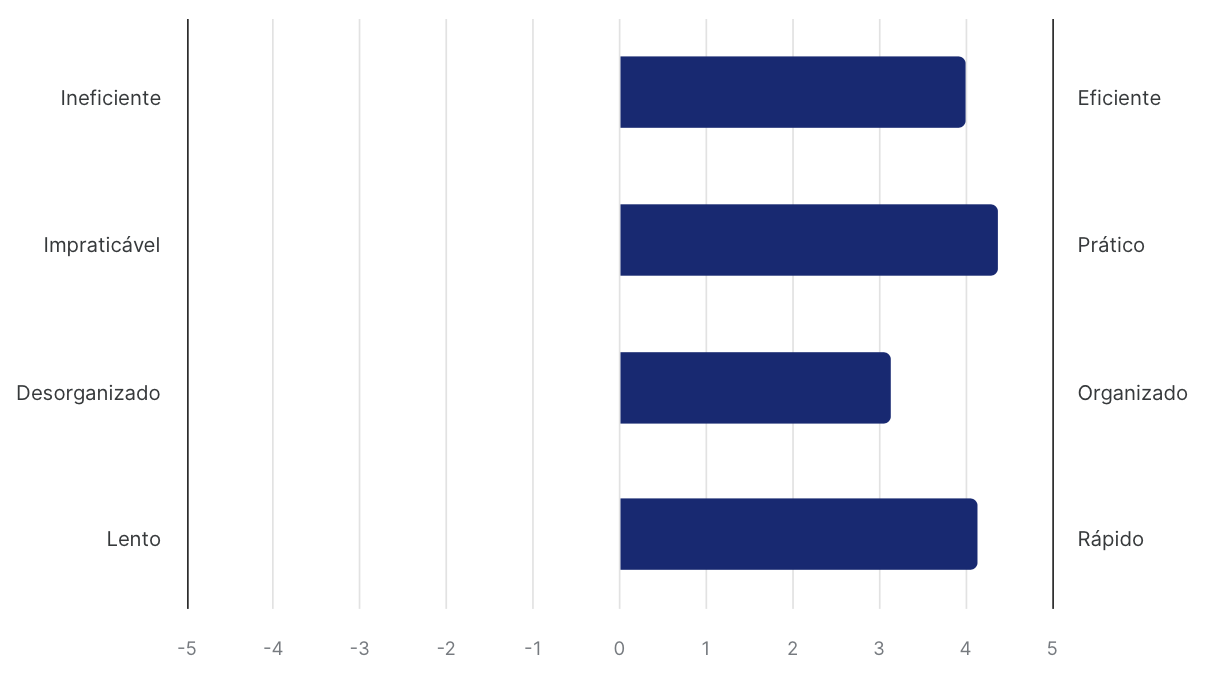
\includegraphics[scale=0.4]{figuras/resultados/ux-5.png}
    \label{fig:ux-5}
    \legend{Fonte: Eonay e Klenilmar (2024).}
\end{figure}

Alguns comentários deixados sobre eficiência na avaliação:
\begin{citacao}

\item "Funcionou no internet explorer sem precisar de login é melhor ainda";
\item "A ferramenta informa quando falta algum campo para preencher";
\item "A entrega dos resultados é rápida e eficiente".

\end{citacao}

Essa eficiência do software é amplamente discutida na engenharia de software por conta das inúmeras variáveis que influenciam neste processo que, neste caro, ocorre geograficamente distante de cada usuário que utiliza e se mantém eficiente, para \citeonline{smith2022software}:

\begin{citacao}
A eficiência do software é um atributo crítico que impacta diretamente o desempenho dos sistemas e a satisfação dos usuários. Programas otimizados reduzem o consumo de recursos computacionais, como tempo de processamento e memória, o que é essencial em sistemas de grande escala ou ambientes com recursos limitados. Além disso, a eficiência contribui para maior sustentabilidade ao minimizar a demanda energética associada ao uso prolongado de dispositivos computacionais.

Adotar práticas de engenharia de software voltadas à eficiência requer uma abordagem multidimensional, combinando design cuidadoso, escolha criteriosa de algoritmos e técnicas de otimização em níveis de código e sistema. Estudos mostram que, embora a busca por eficiência possa aumentar a complexidade inicial do desenvolvimento, ela resulta em benefícios significativos durante a operação e manutenção do software.
\end{citacao}

Todas as características avaliadas anteriormente auxiliam na motivação dos participantes em utilizar, Figura \ref{fig:ux-7}, se tornando motivante e interessante por uma ou mais características excitantes, motivador do apreço ou desapreço ao software.

\begin{figure}[h!]
    \caption{Você se sente motivado a utilizar o produto novamente}
    \centering
    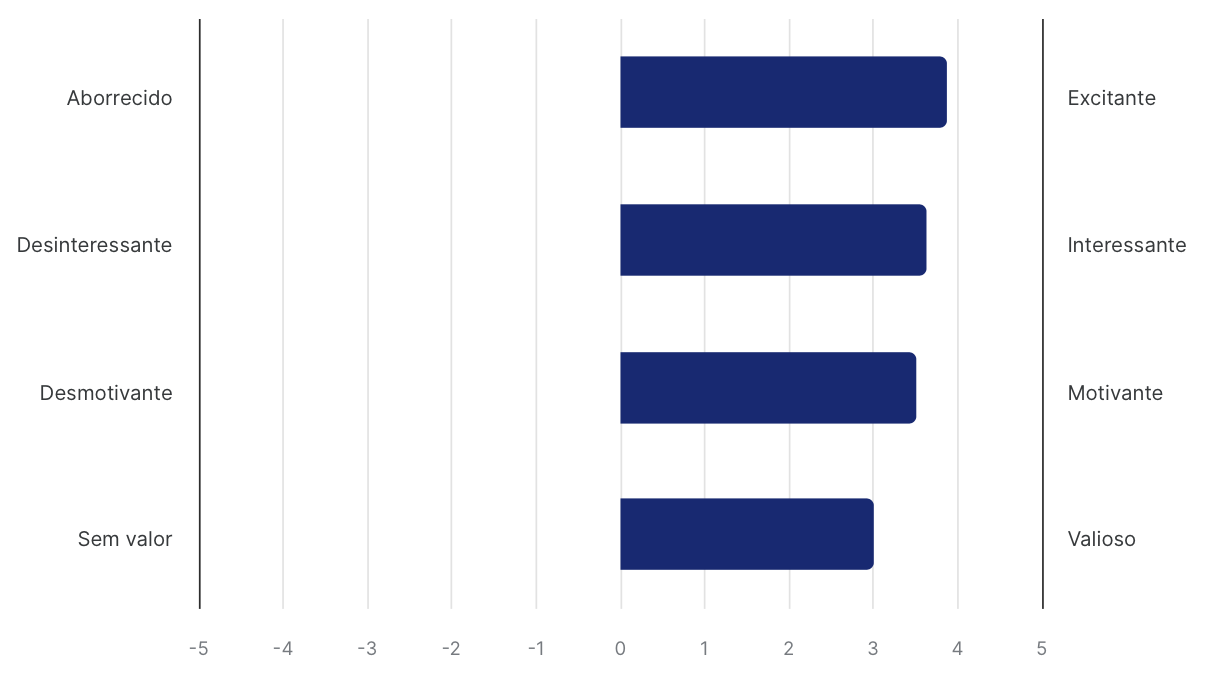
\includegraphics[scale=0.4]{figuras/resultados/ux-7.png}
    \label{fig:ux-7}
    \legend{Fonte: Eonay e Klenilmar (2024).}
\end{figure}


Alguns comentários deixados sobre estimulação na avaliação:
\begin{citacao}
\item "Tem que colocar as outras propriedades que as matrizes possuem";
\item "O Mathix tem potencial de estimular a continuidade do uso da ferramenta, pois habilita a curiosidade de testar cada uma das propriedades/funções disponíveis e de saber como se chegou ao resultado".
\end{citacao}


O uso dessas tecnologias democratiza o acesso a experiências que, de outra forma, poderiam ser limitadas por recursos financeiros ou geográficos. Produtos Educacionais com estimulação de software oferecem oportunidades iguais de aprendizado, independentemente do contexto socioeconômico dos alunos. Assim, ao integrar soluções tecnológicas no ensino, instituições de educação contribuem para a formação de profissionais mais capacitados e preparados para enfrentar os desafios do mundo de trabalho, fortalecendo o papel da tecnologia como um catalisador do aprendizado inclusivo e inovador.

A inovação no desenvolvimento de software tem sido um fator fundamental na criação de ferramentas educacionais que buscam aprimorar o processo de ensino e aprendizagem. A introdução de tecnologias como \textbf{inteligência artificial, gamificação e aprendizado adaptativo} tem permitido que as ferramentas educacionais se tornem mais personalizadas, interativas e eficazes no atendimento das necessidades individuais dos estudantes. Essas inovações possibilitam um ambiente mais dinâmico e atraente, favorecendo a participação ativa e o engajamento dos alunos \cite{santos2022inovacao}. Figura \ref{fig:ux-9} mostra a avaliação no quesito inovação.

\begin{figure}[h!]
    \caption{O produto é inovador e criativo}
    \centering
    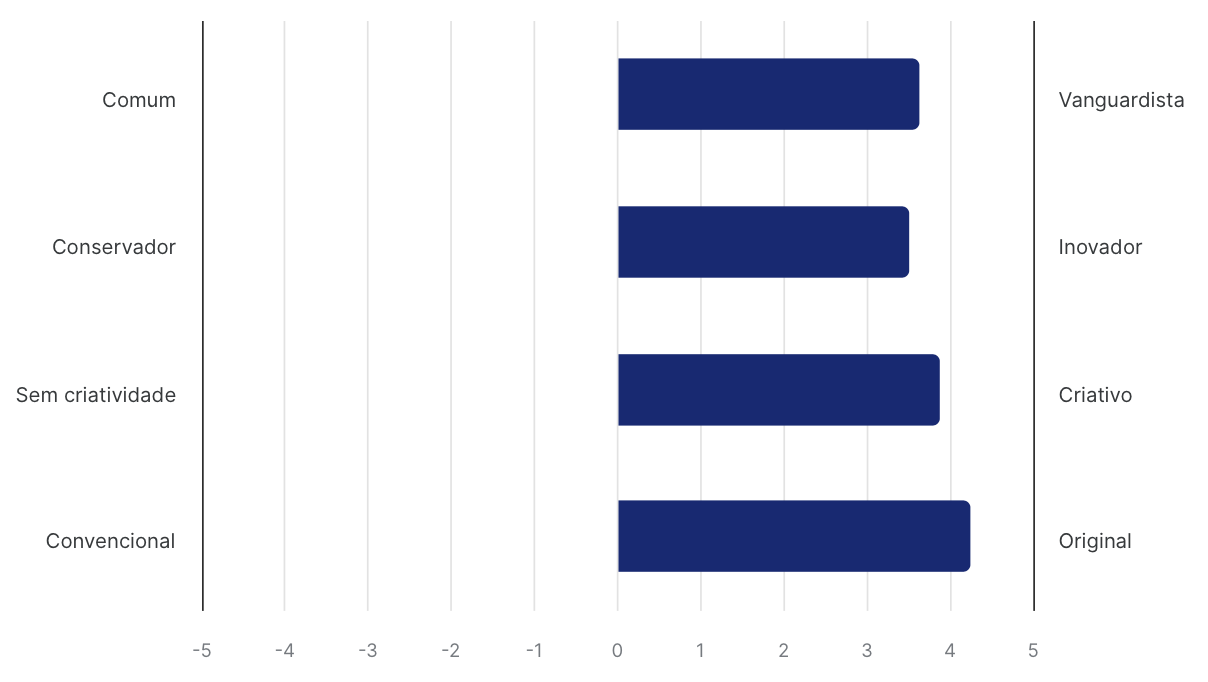
\includegraphics[scale=0.4]{figuras/resultados/ux-9.png}
    \label{fig:ux-9}
    \legend{Fonte: Eonay e Klenilmar (2024).}
\end{figure}

Alguns comentários deixados sobre novidade na avaliação:
\begin{citacao}
\item "Para utilizar matrizes no computador apenas conhecia o matlab que é bem mais completo";
\item "Eu achei inovador, não vejo tantas opções disponíveis de ferramentas com enfoque no assunto matemático explorado pelo Mathix, a maioria é sempre na categoria jogos digitais".
\end{citacao}

A compreensão é fundamental para para a perspicuidade do Mathix como plataforma e de fácil familiaridade principalmente pela questão da interface, Figura \ref{fig:ux-11} traz os resultados da analise sobre a familiaridade e compreensão da proposta.


\begin{figure}[h!]
    \caption{O produto é fácil de entender e de se familiarizar}
    \centering
    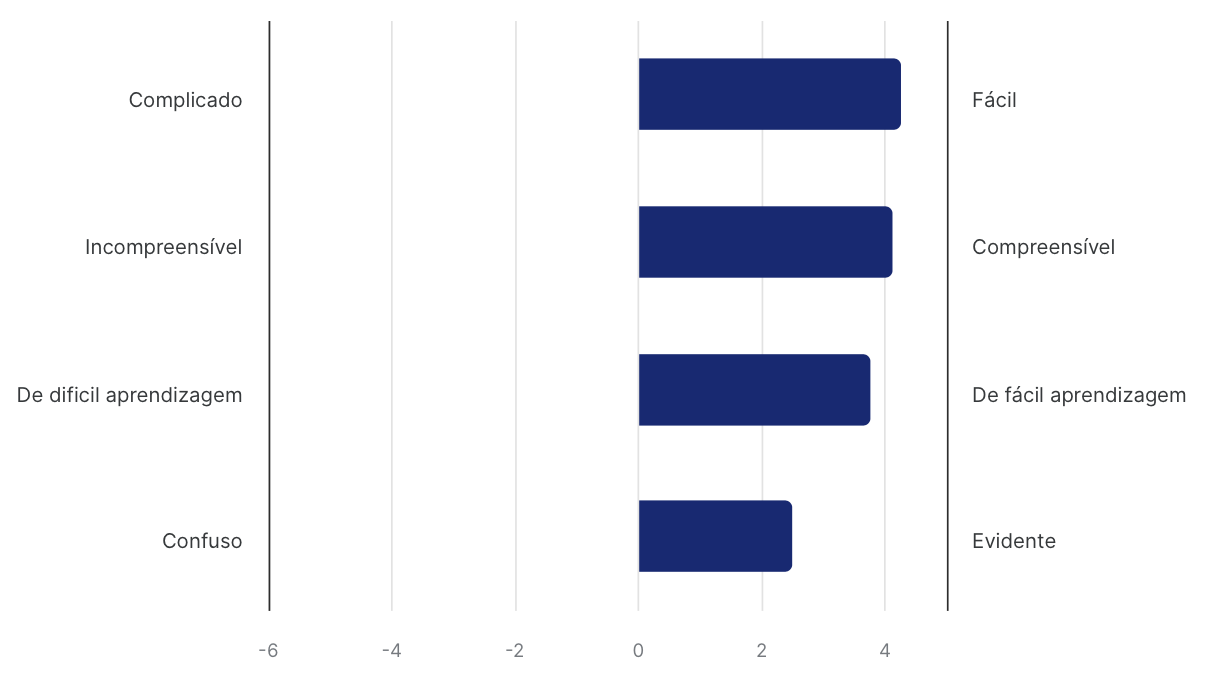
\includegraphics[scale=0.4]{figuras/resultados/ux-11.png}
    \label{fig:ux-11}
    \legend{Fonte: Eonay e Klenilmar (2024).}
\end{figure}

Alguns comentários deixados sobre perspicuidade na avaliação:

\begin{citacao}
\item "Bem direto no que se propõem, pode se tornar melhor com mais recursos";
\item "Achei o produto claro e fácil de entender. Apenas identifiquei que: Se o usuário deixar os campos linhas e colunas vazios não é exibida a mensagem de aviso de que precisa preencher. O usuário consegue digitar o intervalo inicial e intervalo final, ainda que tenha selecionado Valor 0 (zero) ou Valor 1 (um)".
\end{citacao}




De forma geral a avaliação de 1 a 10 para a experiencia do usuário em utilizar o produto educacional na Figura \ref{fig:ux-13}, representado na escala radial que demonstra um alto índice de satisfação no intervalo entre 7 a 10 como resultado indicador de aceitação pelos participantes.

\begin{figure}[h!]
    \caption{Grau de Satisfação do PE (UX)}
    \centering
    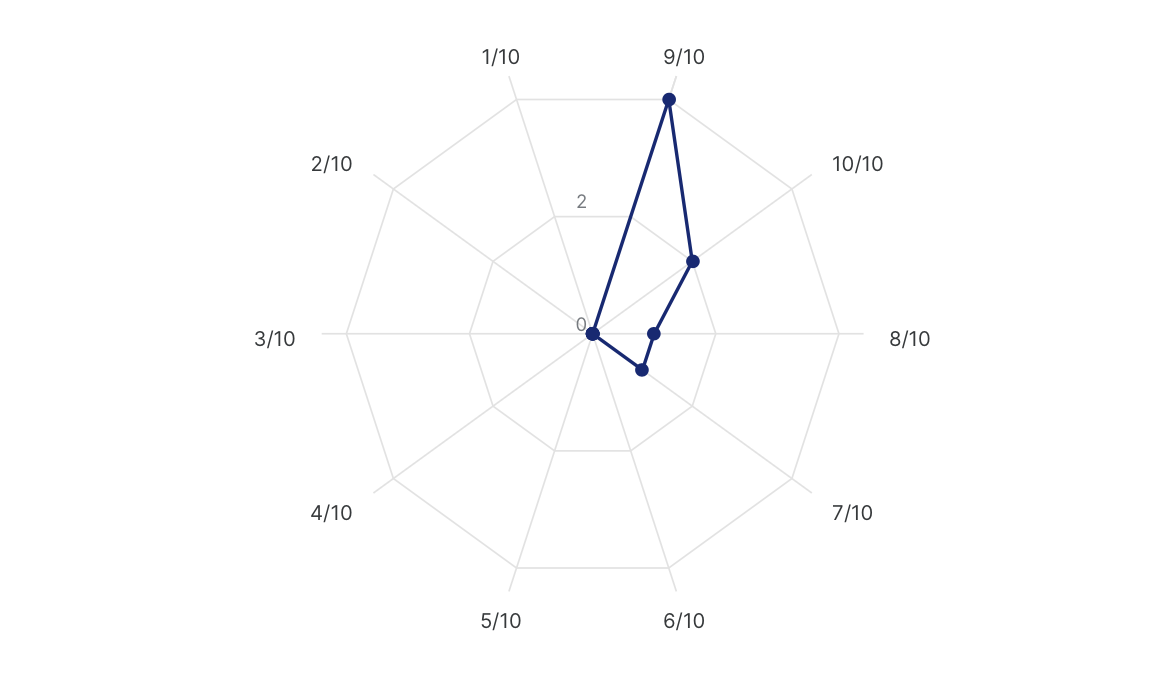
\includegraphics[scale=0.5]{figuras/resultados/satisfacao_ux.png}
    \label{fig:ux-13}
    \legend{Fonte: Eonay e Klenilmar (2024).}
\end{figure}



Por fim de forma optativa fui questionado aos participantes uma avaliação final como pergunta aberta e, obtivemos os \textit{feedbacks}:

\begin{citacao}
    \item "O fato de poder usar via qualquer tipo de dispositivo e de forma gratuita vale a pena";
    \item "Achei fácil de usar e de compreender os resultados".
\end{citacao}













\section{Modelo Acadêmico em LaTeX para ProfEPT IFAP}
\label{model_latex}

O \textbf{LaTeX} é um sistema de preparação de documentos amplamente utilizado em ambientes acadêmicos e científicos, especialmente em áreas que demandam escrita técnica ou matemática. Se baseado na linguagem de marcação \textbf{TeX} e permite criar documentos com alta qualidade tipográfica. O LaTeX é amplamente usado para elaborar artigos, dissertações, teses, e outros tipos de documentos acadêmicos devido à sua precisão e flexibilidade.

Concluir um projeto educacional que envolve a criação de um modelo de documento no formato LaTeX \footnote{https://github.com/eonay/profept-latex}, ajustado às normas da ABNT, é um marco significativo no desenvolvimento de ferramentas para auxiliar acadêmicos e estudantes. Esse tipo de produto educacional não apenas resolve desafios relacionados à padronização, mas também democratiza o acesso a soluções que tornam o processo de escrita científica mais ágil e eficiente. Ao integrar as exigências formais com a praticidade do LaTeX, o modelo se consolida como uma alternativa moderna e poderosa para trabalhos acadêmicos.

O desenvolvimento do modelo LaTeX para ProfEPT com conformidade às normas da ABNT requer uma abordagem meticulosa. Cada detalhe, desde a estrutura básica dos capítulos e sessões até elementos como margens, referências e formatação de citações, precisa ser rigorosamente ajustado. Essa atenção ao detalhe garante que os utilizadores do modelo possam se concentrar no conteúdo, confiando que o formato estará em conformidade com os padrões exigidos pelas instituições e revistas científicas. Assim, o produto educacional não apenas facilita o cumprimento das normas, mas também contribui para a valorização da escrita acadêmica formal.

Além de sua aplicabilidade técnica, o modelo tem potencial pedagógico, pois ajuda estudantes a compreender melhor as diretrizes da ABNT ao utilizá-lo. Como um guia prático, ele funciona como uma ferramenta de aprendizado integrada, permitindo que os usuários vejam na prática como aplicar as regras de formatação, citações e referências. Essa característica transforma o modelo em um recurso valioso para professores e alunos, reforçando a importância da padronização na comunicação científica e promovendo o profissionalismo nos trabalhos apresentados.

A implementação do LaTeX como tecnologia de base adiciona uma camada de relevância ao projeto, pois incentiva a adoção de \textbf{ferramentas computacionais} avançadas no ambiente acadêmico. Apesar de ter uma curva inicial de aprendizado, o LaTeX oferece vantagens significativas, como \textbf{consistência e flexibilidade no design de documentos}. O modelo, ao simplificar a configuração inicial e automatizar aspectos técnicos, torna essa tecnologia mais acessível, especialmente para iniciantes, diminuindo barreiras e estimulando o uso de \textbf{práticas inovadoras no âmbito educacional}.

Por fim, a conclusão desse produto representa uma síntese do esforço \textbf{técnico e educacional}. Ele não apenas resolve problemas práticos enfrentados por acadêmicos, mas também fomenta uma cultura de excelência na produção científica e tecnológica. O impacto positivo de um modelo LaTeX com ajustes às normas da ABNT vai além de facilitar a conformidade normativa, ele promove a integração de tecnologias modernas com a educação, transformando o processo de criação acadêmica em algo mais \textbf{eficiente e acessível} a todos.










\chapter{Conclusão}
\label{conclusao}

Com os resultados obtidos nesta pesquisa, pode-se concluir que a utilização de software como ferramenta de suporte e apoio no ensino de matrizes é uma estratégia educacional promissora com potencialidade promover um melhor processo de ensino-aprendizagem mais significativo.

O software Mathix permitiu visualizar e manipular de maneira interativa e dinâmica mesmo que em sua versão inicial, o que contribuiu para o desenvolvimento do raciocínio lógico de forma lúdica, criativa e da autonomia dos estudantes durante as atividades. Além disso, pode proporcionar aos alunos uma melhor compreensão do conteúdo de matriz no cotidiano e em sua futura atuação profissional inclusive como futuros docentes.


Assim sendo, é imprescindível reconsiderar as práticas pedagógicas no ensino de matrizes. A utilização da tecnologia deve ser encarada como uma ferramenta benéfica, não como um obstáculo, visando enriquecer as aulas de forma significativa. A adoção de softwares, como o Mathix, pode se transformar em um aliado nesse processo. Dessa forma, o professor pode explorar novos recursos e métodos de ensino, promovendo a eficácia das aulas e captando a atenção dos alunos, resultando em desempenhos positivos.


Em síntese, para que o uso dessas ferramentas educacionais seja eficaz, é crucial que os professores recebam formação contínua, adquirindo o conhecimento necessário para manipular novas tecnologias em suas práticas. Além disso, é essencial que as atividades sejam cuidadosamente planejadas para atender aos diferentes níveis de aprendizagem dos alunos. Por fim, as situações-problema devem ser contextualizadas, relacionando-se com espaços e situações reais, a fim de serem significativas e motivadoras.

O uso de ferramentas de mediação educacionais representam um passo importante na democratização dos espaços e no acesso à tecnologia, embora ainda exija discussões contínuas sobre suas potencialidades e limitações. Compreender as experiências e os conceitos por trás dessas ferramentas para diferentes grupos em cursos é fundamental para direcionar futuras pesquisas.


Portanto, espera-se que o conteúdo desta pesquisa, aliado ao produto educacional desenvolvido, contribua para incentivar a adoção de uma abordagem integrada e abrangente para aplicação de tecnologias na educação, facilitando a aplicação dos conhecimentos científicos adquiridos em outras disciplinas e no mundo de trabalho.



%%========== Section ==========%
\section{Publicações Submetidas}
\label{publicacoes}

A proposta e a metodologia de pesquisa, bem como os resultados obtidos, foram submetidos para avaliação, com o objetivo de fortalecer a credibilidade do estudo. As submissões listadas a seguir ocorreram em momentos distintos, respeitando a ordem cronológica do desenvolvimento da pesquisa.

Os trabalhos resultaram tanto das metodologias propostas quanto dos resultados alcançados, sendo ambos aceitos para apresentação em um evento nacional:

\begin{enumerate}
   \item CNMAC 2023 - XLII Congresso Nacional de Matemática Aplicada e Computacional. 18 à 22 de Setembro de 2023 - Bonito - MS;

   \item SENACEM 2024 - VIII Seminário Nacional do Ensino Médio e III Simpósio Interdisciplinar. 27, 28 e 29 de Novembro de 2024 - Mossoró - RN.
\end{enumerate}




%%========== Section ==========%
\section{Limitações}
\label{limitacoes}

A versão inicial da ferramenta foi projetada para abordar aspectos fundamentais do ensino de matrizes, oferecendo uma base sólida para a futura implementação de novas operações relacionadas a esse tópico. A estrutura desenvolvida busca atender às necessidades iniciais, enquanto mantém espaço para expansão e aprimoramento conforme o uso e \textit{feedback} dos usuários.

Como a aplicação foi desenvolvida no formato de plataforma, a documentação explicativa anexada à ferramenta ainda é limitada. Esse é um ponto a ser aprimorado para garantir que os usuários compreendam plenamente as funcionalidades disponíveis e como utilizá-las de maneira eficiente.

Outro aspecto importante a ser considerado é a capacidade da ferramenta de lidar com múltiplos acessos simultâneos. É essencial realizar testes de desempenho e carga para avaliar a robustez da aplicação em cenários de alta demanda, garantindo sua estabilidade e eficiência mesmo em situações de uso intenso.

%%========== Section ==========%
\section{Trabalhos Futuros}
\label{trabalhos_futuros}

Entre as perspectivas futuras para esta pesquisa, destaca-se a aplicação da matemática em contextos de outros cursos técnicos, visando otimizar estruturas e maximizar o aproveitamento de materiais em diversas áreas. As competências envolvidas possibilitam a exploração desses aspectos de maneira viável, colaborativa e transdisciplinar.

A possibilidade de interação com outras ferramentas educacionais e um incentivo ao uso de tecnologias baseadas em software livre, segundo \citeonline{martins2021software} “software livre” devemos entender aquele software que respeita a liberdade e senso de comunidade dos usuários. A grosso modo, isso significa que os usuários possuem a liberdade de executar, copiar, distribuir, estudar, mudar e melhorar o software.





% ----------------------------------------------------------
% -- Elementos Pós-Textuais: -------------------------------
\postextual  
\bibliography{referencias} % Referências bibliográficas
%-------------------------------------------------------------
%---------------------- Apêndices ----------------------------
%-------------------------------------------------------------

\begin{apendicesenv}
\partapendices  % Indica o início dos Apendices
\chapter{Termo de Consentimento Livre e Esclarecido (TCLE)}

\begin{center}
\textbf{Termo de Consentimento Livre e Esclarecido (TCLE)}
\end{center}


Prezado (a) Senhor (a):
Gostaríamos de convidar sob sua responsabilidade para participar do Projeto de pesquisa do Instituto Federal do Amapá - IFAP. O Projeto com o título Práticas de Ensino com Matrizes, será realizado no Câmpus Macapá, sendo conduzido pelo pesquisador identificado neste documento. O objetivo e mapear as ferramentas mais aplicadas para ensino de matrizes; analisar o uso de ferramentas aplicadas com matrizes; classificar recursos aplicados a matrizes nos planos de aula.

Os sujeitos pesquisados serão os docentes da unidade de Macapá-AP
do Curso de Licenciatura em Matemática. A participação docente é muito importante e ela se daria no ano de 2023 e ou 2024.
Logo em seguida será solicitado a cada participante que responda um breve questionário.

Esclarecemos que a participação do docente é totalmente voluntária, podendo o(a) senhor(a) solicitar a recusa ou desistência de participação a qualquer
momento, sem que isto acarrete qualquer ônus ou prejuízo. Esclarecemos,
também, que as informações prestadas serão utilizadas somente para os fins de pesquisa (ou para esta e futuras pesquisas) e serão tratadas com o mais absoluto sigilo e confidencialidade, de modo a preservar a identidade do docente. Os dados levantados ficarão sob a guarda do pesquisador por um período de cinco anos e, após esse tempo, os instrumentos de coletas de dados em mídia e ou em papel serão picotados/destruídos e encaminhados à reciclagem. Em relação aos riscos dos participantes da pesquisa podem se sentir inibidos durante a participação ao responder ao questionário. Objetivando evitar ou diminuir tais riscos aos docentes serão avisados que podem solicitar esclarecimento de qualquer dúvida (antes, durante ou depois da pesquisa), de forma individual, ou mesmo desistir da participação a qualquer momento. Esclarecemos ainda, que nem o(a) senhor(a) pagarão ou serão remunerados (as) pela participação, sendo a mesma de forma voluntária.



Garantimos, no entanto, que todas as despesas decorrentes da pesquisa serão financiadas pelo pesquisador. Como benefício gerado por essa pesquisa, espera-se com a conclusão deste projeto, inicialmente incentivar e promover a adoção de produtos educacionais na prática docente assim como métodos científicos e de pesquisa para a produção.



Contudo, tenho sido devidamente esclarecido sobre os procedimentos da
pesquisa, concordo com a participação voluntariada sob minha responsabilidade na pesquisa descrita acima. As suas respostas  não serão divulgadas de forma a possibilitar a identificação, sendo guardadas em sigilo.

Caso o(a) senhor(a) tenha dúvidas ou necessite de maiores esclarecimentos poderá contactar o pesquisador responsável pelo e-mail eonay.web@gmail.com, ou por telefone (96) 99122-4131.



\hfill \break
\begin{center}
\rule{90mm}{1pt}

Participante Voluntário(a) [Assinatura]
\end{center}

\hfill \break
\begin{center}
\rule{90mm}{1pt}

Telefone e ou E-mail do Participante Voluntário
\end{center}


\hfill \break

Em caso de dúvidas com respeito aos aspectos éticos deste estudo, poderei consultar:
\newline
\newline
Comitê de Ética em Pesquisa da Universidade Estadual do Amapá - CEP/UEAP
\newline 
E-mail: cep@ueap.edu.br
\newline 
Endereço: Avenida FAB esquina com Tiradentes, Centro, AP, CEP: 68.900-098
\newline 
Telefone: (96) 99116-9811
\newline
\hfill
\newline
Pesquisador(a): Eonay Barbosa Gurjão
\newline
Telefone para contato: (96) 99122-4131
\newline
E-mail para contato: eonay.web@gmail.com
\newline
Orientador(a): Klenilmar Lopes Dias
\newline
\newline
Número do CAAE\footnote{Certificado de Apresentação de Apreciação Ética}: 70930823.6.0000.0211







\chapter{Ficha de Avaliação de Experiência do Usuário}


\begin{center}
\textbf{
Ficha de Avaliação de Experiência do Usuário\\
Adaptado de \citeonline{laugwitz2008construction}
}
\end{center}
E-mail do Avaliador:\hrulefill \\
Usuário Avaliador: \hrulefill \\

\begin{center}
Produto Avaliado: Mathix    
\end{center}


Considerando os itens que mensuram diretamente a atratividade visual, bem como a qualidade dos aspectos ergonômicos, defina uma opção de acordo com a sua experiência de uso do produto educacional:





\begin{enumerate}
    
    \item Atratividade\\Você gostou ou não do produto?
    \begin{enumerate}
        \item ( ) Desagradável OU ( ) Agradável
        \item ( ) Feio OU ( ) Atraente
        \item ( ) Desinteressante OU ( ) Atrativo
        \item ( ) Bom OU ( ) Ruim
        \item Comentários sobre a Atratividade:\hrulefill \\     
        \rule{14cm}{.1pt}\\
        \rule{14cm}{.1pt}\\
            
    \end{enumerate}

    
    \item Controle\\Você se sente no controle da situação durante a interação?
    \begin{enumerate}
        \item ( ) Não atende às expectativas OU ( ) Atende as expectativas
        \item ( ) Imprevisível OU ( ) Previsível
        \item ( ) Desinteressante OU ( ) Atrativo
        \item ( ) Inseguro OU ( ) Seguro
        \item Comentários sobre o Controle:\hrulefill \\     
        \rule{14cm}{.1pt}\\
        \rule{14cm}{.1pt}\\
              
    \end{enumerate}


    \item Eficiência\\O produto pode ser utilizado de maneira fácil e eficiente?
    \begin{enumerate}
        \item ( ) Ineficiente OU ( ) Eficiente
        \item ( ) Impraticável OU ( ) Prático
        \item ( ) Desorganizado OU ( ) Organizado
        \item( ) Lento OU ( ) Rápido
        \item Comentários sobre o Eficiência:\hrulefill \\     
        \rule{14cm}{.1pt}\\
        \rule{14cm}{.1pt}\\
        
    \end{enumerate}


    \item Estimulação\\Você se sente motivado a utilizar o produto novamente?
    \begin{enumerate}
        \item ( ) Aborrecido OU ( ) Excitante
        \item ( ) Desinteressante OU ( ) Interessante
        \item ( ) Desmotivante OU ( ) Motivante
        \item ( ) Sem valor OU ( ) Valioso
        \item Comentários sobre a Estimulação:\hrulefill \\      
        \rule{14cm}{.1pt}\\
        \rule{14cm}{.1pt}\\
        
    \end{enumerate}
    
    \item Novidade\\O produto é inovador e criativo?
    \begin{enumerate}
        \item ( ) Comum OU ( ) Vanguardista
        \item ( ) Conservador OU ( ) Inovador
        \item ( ) Sem criatividade OU ( ) Criativo
        \item ( ) Convencional OU ( ) Original
        \item Comentários sobre a Novidade:\hrulefill \\     
        \rule{14cm}{.1pt}\\
        \rule{14cm}{.1pt}\\
    \end{enumerate}

    \item Perspicuidade\\O produto é fácil de entender e de se familiarizar?
    \begin{enumerate}
        \item ( ) Complicado OU ( ) Fácil
        \item ( ) Incompreensível OU ( ) Compreensível
        \item ( ) De difícil aprendizagem OU ( ) De fácil aprendizagem
        \item ( ) Confuso OU ( ) Evidente 
        \item Comentários sobre a Perspicuidade:\hrulefill \\       
        \rule{14cm}{.1pt}\\
        \rule{14cm}{.1pt}\\
        
    \end{enumerate}

    
\end{enumerate}

Por fim, atribua uma pontuação a fim de definir o Grau de Experiência de uso do produto avaliado.
PONTUAÇÃO FINAL DA AVALIAÇÃO: NOTA (0 à 10) NOTA:(\space\space\space\space)
\\
\\
\\
   PARECER FINAL DO(A) AVALIADOR(A):\hrulefill \\
        \rule{16cm}{.1pt}\\
        \rule{16cm}{.1pt}\\
        \rule{16cm}{.1pt}\\
        \rule{16cm}{.1pt}\\
        

















\chapter{Ficha de Avaliação de Interface para Usuário}

\begin{center}
\textbf{
Ficha de Avaliação de Interface para Usuário\\
Adaptado de \citeonline{preece2015interaction}
}
\end{center}
E-mail do Avaliador: \hrulefill \\
Usuário Avaliador: \hrulefill \\

\begin{center}
Produto Avaliado: Mathix    
\end{center}


Considerando os itens que mensuram diretamente a satisfação de interação com a interface para uso do produto educacional:




\begin{enumerate}
    
    \item Quão fácil foi instalar o nosso o Mathix?
    \begin{enumerate}
        \item ( ) Extremamente fácil
        \item ( ) Moderadamente fácil
        \item ( ) Nada fácil\\
    \end{enumerate}


    \item Quão fácil de ser usada é a interface do software?
    \begin{enumerate}
        \item ( ) Extremamente fácil
        \item ( ) Muito fácil
        \item ( ) Moderadamente fácil
        \item ( ) Não muito fácil
        \item ( ) Nada fácil            
    \end{enumerate}


    \item Com que frequência o Mathix costuma congelar ou falhar?
    \begin{enumerate}
        \item ( ) Constantemente
        \item ( ) Frequentemente
        \item ( ) Ainda não sei (usuário novo)
        \item ( ) Ocasionalmente
        \item ( ) Nunca          
    \end{enumerate}


    \item Qual é a sua opinião geral sobre o desempenho do Mathix?
    \begin{enumerate}
        \item ( ) Ótimo
        \item ( ) Bom
        \item ( ) Regular
        \item ( ) Ruim
        \item ( ) Péssimo
    \end{enumerate}


    \item Qual é a probabilidade de você recomendar o software para outros docentes?
    \begin{enumerate}
        \item ( ) Extremamente alta 100\%
        \item ( ) Muito alta 75\%
        \item ( ) Talvez sim, talvez não 50\%
        \item ( ) Baixa 25\%
        \item ( ) Nenhuma 0\%
    \end{enumerate}


    \item Por favor, diga-nos em suas próprias palavras, quais aspectos do Mathix precisamos melhorar (em 500 caracteres):\hrulefill \\
    \rule{15cm}{.1pt}\\
    \rule{15cm}{.1pt}\\
    \rule{15cm}{.1pt}\\
    
\end{enumerate}

Por fim, atribua uma pontuações para definir o Grau de Satisfação para com uso do produto avaliado.
PONTUAÇÃO FINAL DA AVALIAÇÃO: NOTA (0 à 10) NOTA:(\space\space\space\space)
\\
\\
\\
   PARECER FINAL DO(A) AVALIADOR(A):\hrulefill \\
        \rule{16cm}{.1pt}\\
        \rule{16cm}{.1pt}\\
        \rule{16cm}{.1pt}\\
        \rule{16cm}{.1pt}\\
        









\chapter{Ficha de Avaliação de Pré Diagnostico e Sócio Tecnológica}

\begin{center}
\textbf{
Ficha de Avaliação de Pré Diagnostico e Sócio Tecnológica
}
\end{center}
E-mail do Avaliador:\hrulefill \\
Usuário Avaliador:\hrulefill \\

\begin{center}
Avaliado Individual    
\end{center}


Considerando os itens que mensuram diretamente sua prática docente responda:




\begin{enumerate}

    \item Sua idade em anos (número)?
    \begin{enumerate}
        \item \rule{4cm}{.1pt}\\
    \end{enumerate}


    \item Seu gênero?
    \begin{enumerate}
        \item ( ) Masculino
        \item ( ) Feminino
    \end{enumerate}
    
    
    \item Já trabalhou com o conteúdo de matrizes em alguma disciplina?
    \begin{enumerate}
        \item ( ) Não
        \item ( ) Sim
    \end{enumerate}


    \item Conhece alguma software/aplicativo para trabalhar com matrizes?
    \begin{enumerate}
        \item ( ) Não
        \item ( ) Sim, quais são? \hrulefill \\
          
    \end{enumerate}


    \item Possui acesso a internet?
    \begin{enumerate}
        \item ( ) Apenas no trabalho
        \item ( ) Apenas em casa
        \item ( ) Ambos (casa e trabalho)
        \item ( ) Sem acesso a internet
    \end{enumerate}


    \item Qual o dispositivo mais utilizado para acesso a internet?
    \begin{enumerate}
        \item ( ) Mobile (smatphone)
        \item ( ) Computador de mesa (desktop)
        \item ( ) Computador portátil (laptop ou notebook)
        \item ( ) Tablet
        \item ( ) Outros
    \end{enumerate}


    \item Já utilizou algum software/aplicativo em sua prática docente?
    \begin{enumerate}
        \item ( ) Nunca
        \item ( ) Raramente
        \item ( ) Às vezes
        \item ( ) Muito
        \item ( ) Sempre
    \end{enumerate}


    \item Na sua perspectiva é possível ensinar o conteúdo básico de matrizes com software aplicativo?
    \begin{enumerate}
        \item ( ) Abstenho-me
        \item ( ) Concordo completamente
        \item ( ) Discordo completamente
    \end{enumerate}


    \item Como você avalia o uso de softwares/aplicativos educacionais no ensino?
    \begin{enumerate}
        \item ( ) Insatisfatório
        \item ( ) Regular
        \item ( ) Satisfatório
        \item ( ) Muito Satisfatório
    \end{enumerate}
    
    
\end{enumerate}






\chapter{Ficha de Avaliação do Produto Educacional}

\begin{center}
\textbf{
Ficha de Avaliação do Produto Educacional
}
\end{center}
E-mail do Avaliador:\hrulefill \\
Usuário Avaliador: \hrulefill \\

\begin{center}
Avaliado Individual  
\end{center}


Considerando os itens que mensuram diretamente o produto educacional Mathix, responda:


\begin{enumerate}

    \item Uma nota de 0 à 10 para produto educacional?
    \begin{enumerate}
        \item \rule{4cm}{.1pt}\\
    \end{enumerate}


    \item O produto educacional deve ser utilizado no ensino?
    \begin{enumerate}
        \item ( ) Sim
        \item ( ) Não
    \end{enumerate}
    
    
    \item Você utilizaria o produto educacional em sua prática docente?
    \begin{enumerate}
        \item ( ) Não
        \item ( ) Sim
    \end{enumerate}


    \item De forma geral, sua satisfação ao utilizar o produto educacional na forma software/aplicativo?
    \begin{enumerate}
        \item ( ) Insatisfatório
        \item ( ) Regular
        \item ( ) Satisfatório
        \item ( ) Muito Satisfatório
    \end{enumerate}


    \item Surgiu alguma dificuldade em manusear o produto educacional?
    \begin{enumerate}
        \item ( ) Sim
        \item ( ) Não
    \end{enumerate}


    \item A aplicação propôs a fazer a função para qual foi desenvolvido?
    \begin{enumerate}
        \item ( ) Insatisfatório
        \item ( ) Regular
        \item ( ) Satisfatório
        \item ( ) Muito Satisfatório
    \end{enumerate}
    

   \item Por favor, diga-nos em suas próprias palavras, quais aspectos no produto educacional precisamos melhorar (em 500 caracteres):\hrulefill \\
    \rule{15cm}{.1pt}\\
    \rule{15cm}{.1pt}\\
    \rule{15cm}{.1pt}\\




    
\end{enumerate}





\chapter{Descrição Técnica do Produto Educacional}

\begin{center}
    \textbf{ Descrição Técnica do Produto Educacional}
\end{center}

\begin{flushleft}


\textbf{Origem do produto}: Trabalho de Dissertação “Prática de Ensino com Matrizes”.

\textbf{Área de conhecimento}: Ensino. Linha de Práticas Educativas em EPT.

\textbf{Público Alvo}: Professores da Educação Básica, Técnica e Tecnológica - EBTT e demais interessados em temas referentes ao trabalho docente com ferramentas educacionais.

\textbf{Categoria deste produto}: Ferramenta educacional aberta para auxilio no ensino introdutório de matrizes.

\textbf{Estruturação do Produto}: Este produto é uma software multiplataforma para interação professor e aluno para prática pedagógica interativa dinamicamente adaptada.

\textbf{Registro do Produto/Ano}: Biblioteca do Campus Santana do IFAP, 2024.

\textbf{Avaliação do Produto}: 3 (três) professores que compuseram a Banca de Defesa da Dissertação.

 \textbf{Disponibilidade}: Irrestrita, preservando-se os direitos autorais bem como a proibição do uso comercial do produto.

\textbf{Divulgação}: Em formato digital.

\textbf{Instituições envolvidas}: Instituto Federal do Amapá, Campus Santana e Campus Macapá.

\textbf{URL}: http://eonay.ddns.net:8000

\textbf{Idioma}: Português

\textbf{Cidade}: Santana

\textbf{País}: Brasil
\end{flushleft}




\end{apendicesenv}
%----------------------------------------------------------------
%---------------------- Anexos ----------------------------------
%----------------------------------------------------------------

\begin{anexosenv}
\partanexos   % indica o início dos anexos

% Anexo 01
\chapter{Comitê de Ética em Pesquisa}
\begin{center}
    Documento emitido via Plataforma Brasil do Ministério da Saúde.    
\end{center}

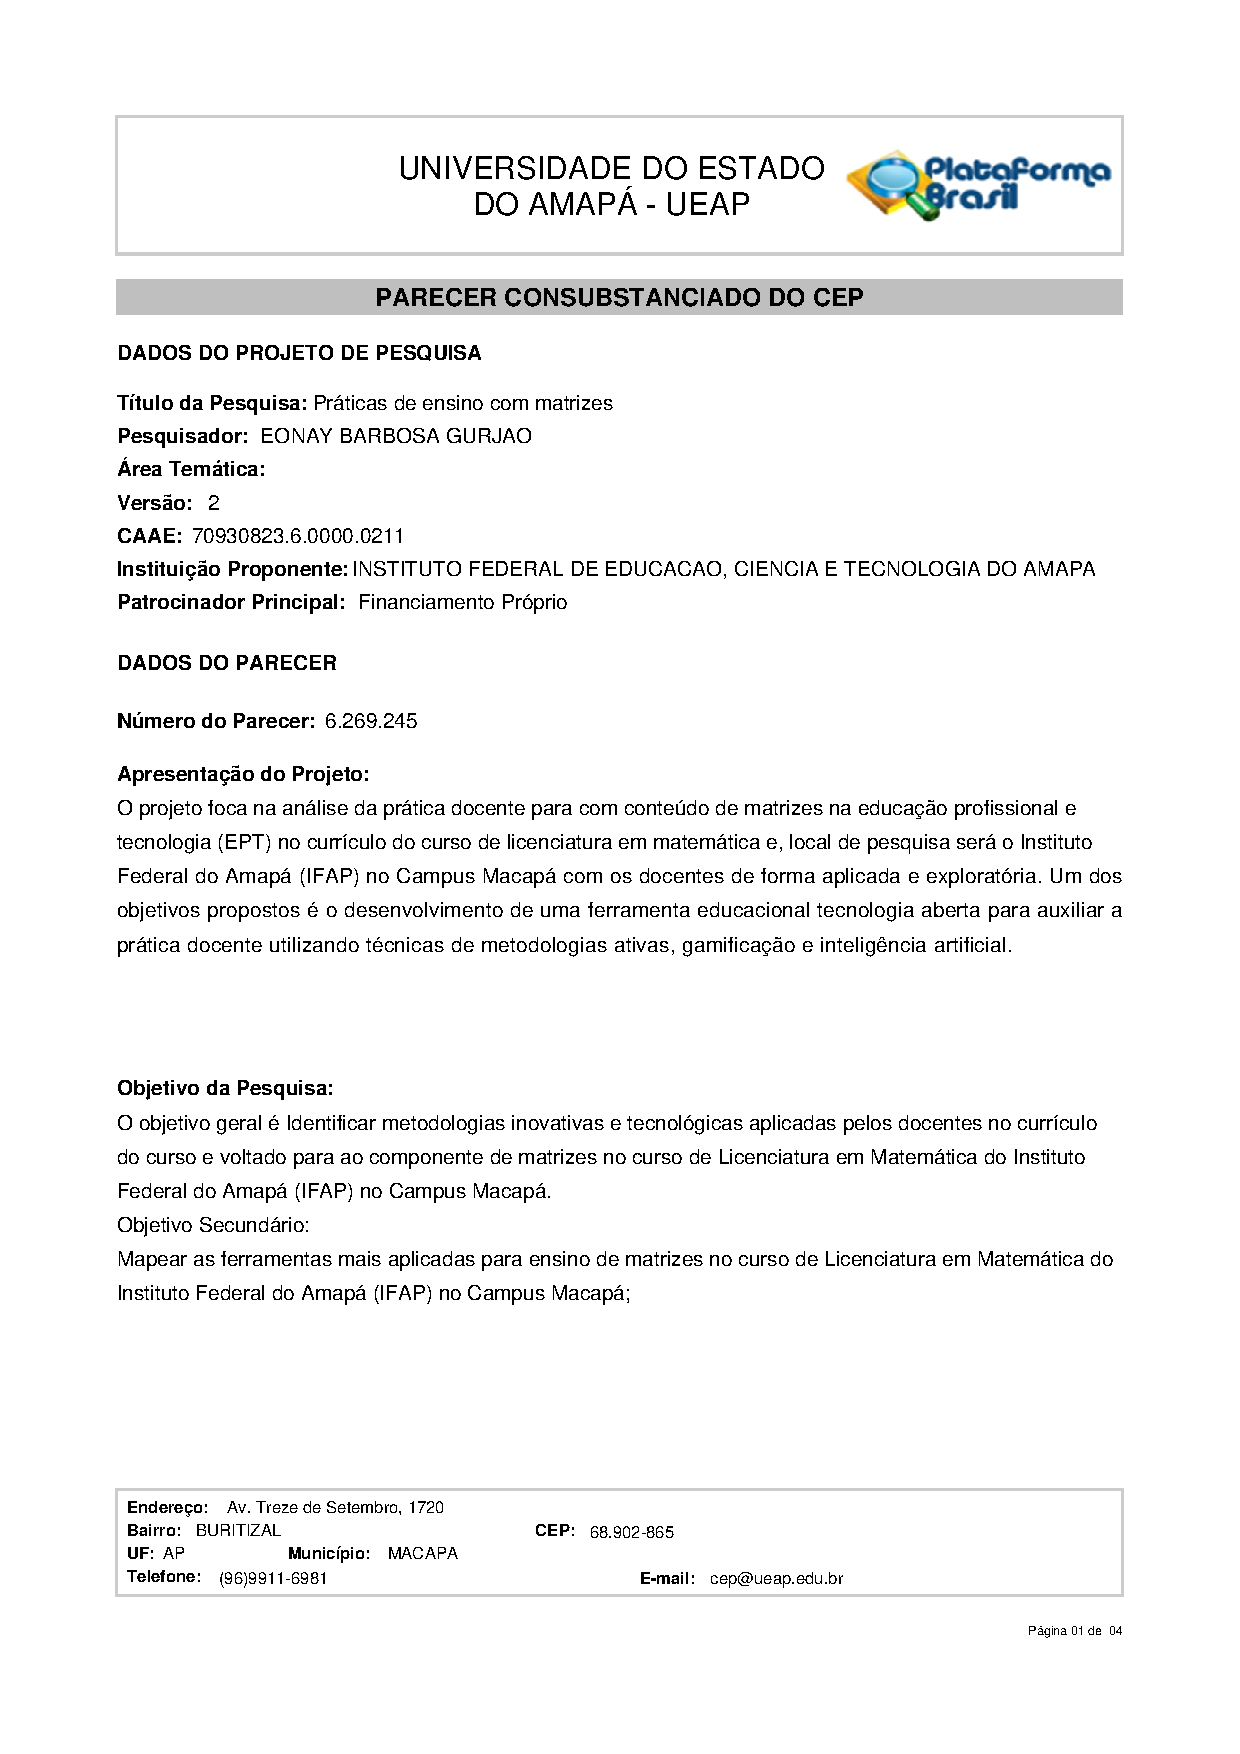
\includepdf[pages=-]{PosTextuais/cep.pdf}


% Anexo 02
\chapter{Termo de Anuência Institucional}
\begin{center}
    Documento emitido via Sistema Unificado de Administração Pública - SUAP do Instituto Federal do Amapá - IFAP.    
\end{center}
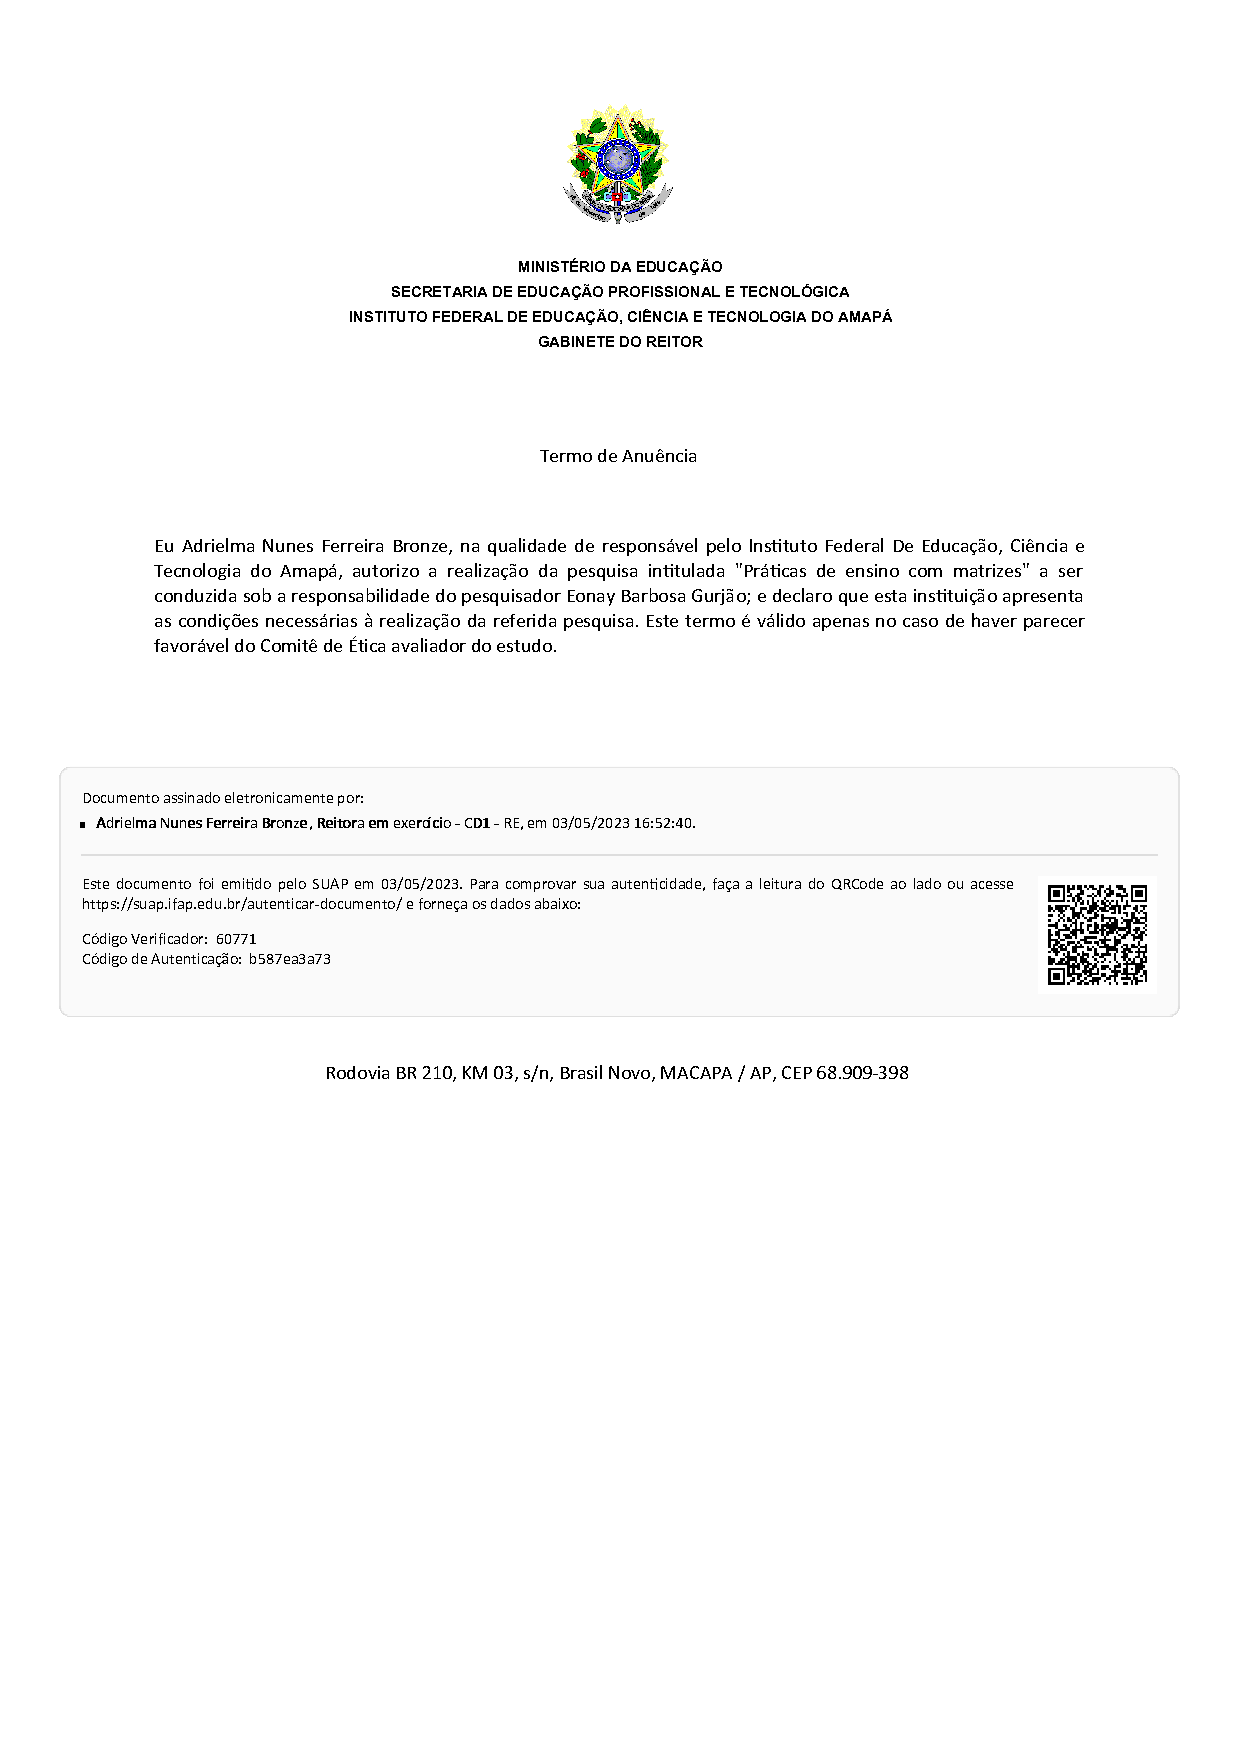
\includepdf[pages=-]{PosTextuais/anuencia.pdf}


% Anexo 03
\chapter{Submissão CNMAC 2023}
\begin{center}
    Documento recebido via Email com o aceite de artigo submetido.    
\end{center}
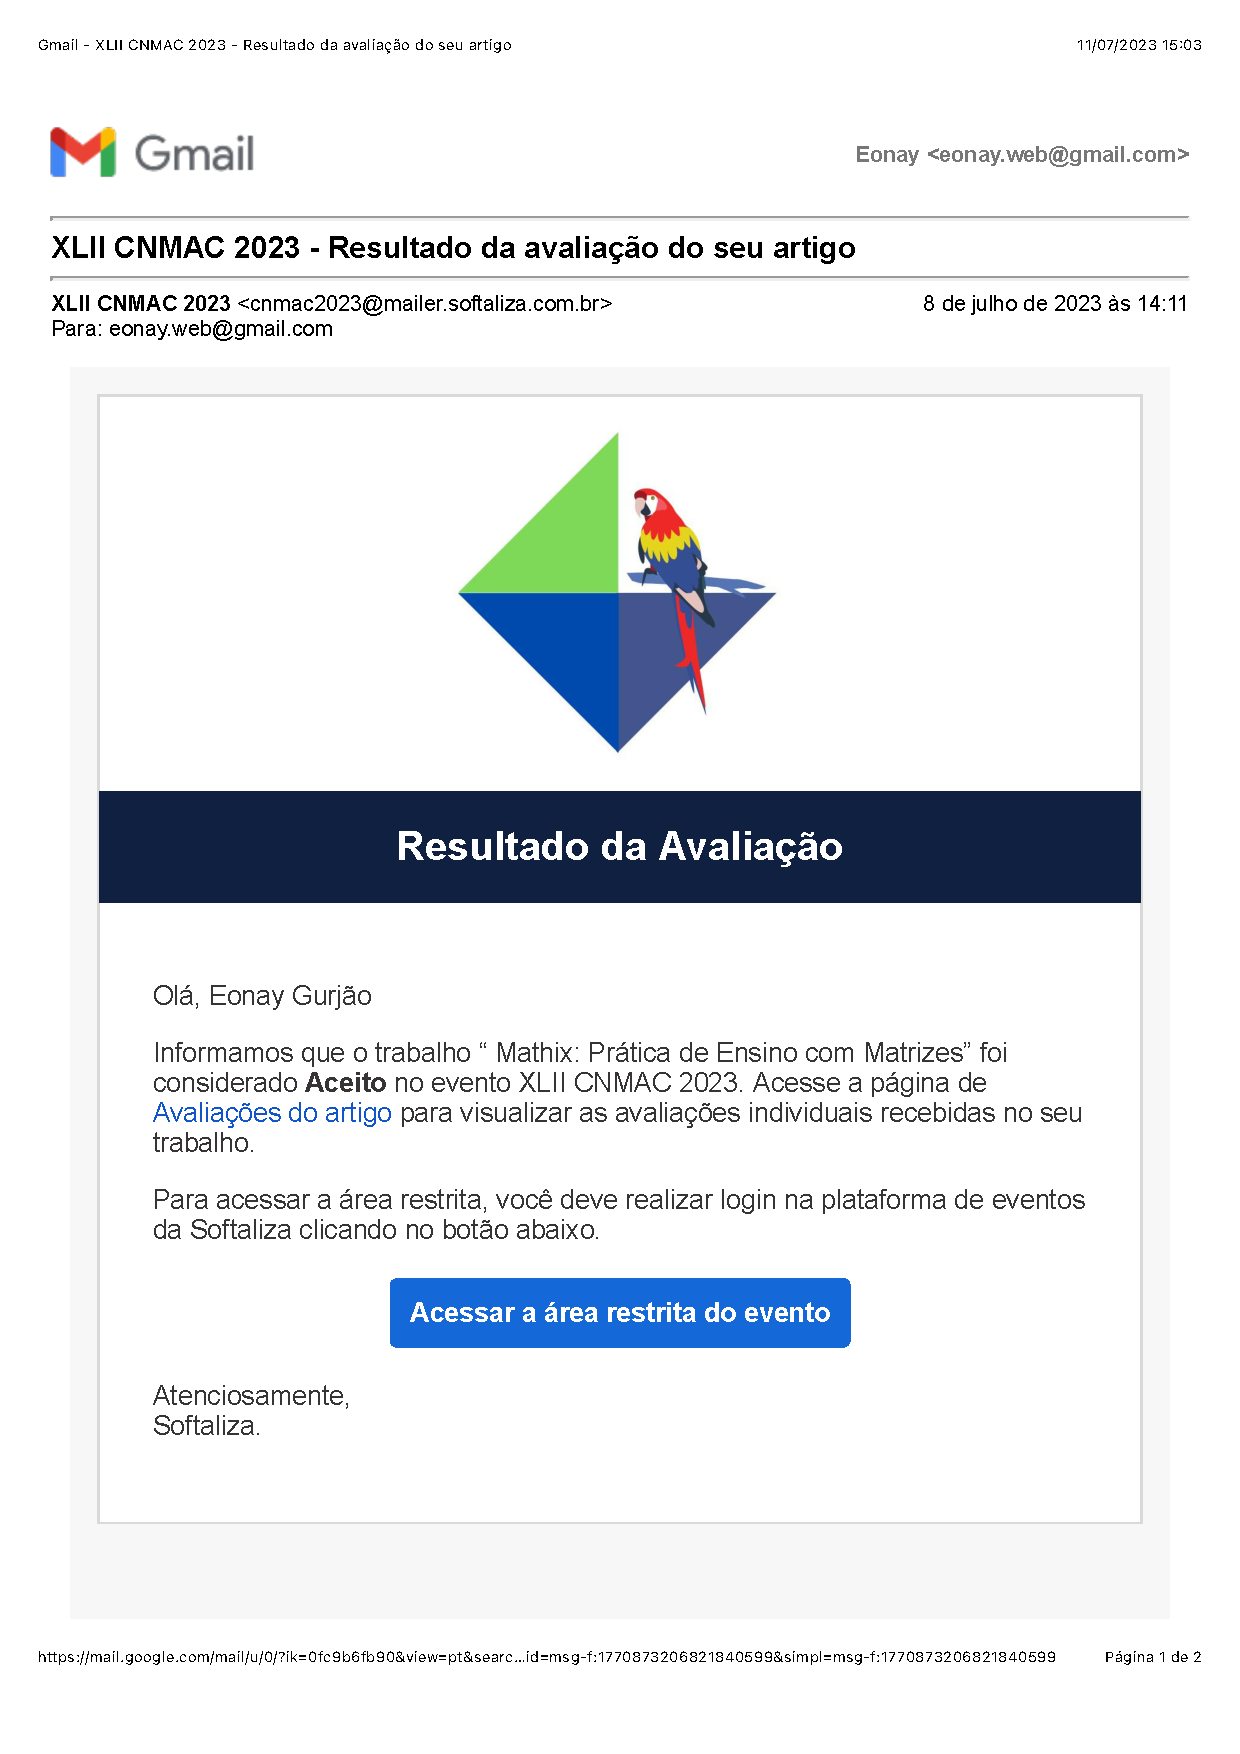
\includepdf[pages=-]{PosTextuais/submissao1.pdf}


% Anexo 04
\chapter{Submissão SENACEM 2024}
\begin{center}
    Documento recebido via Email para com a submissao do artigo para avaliação.    
\end{center}
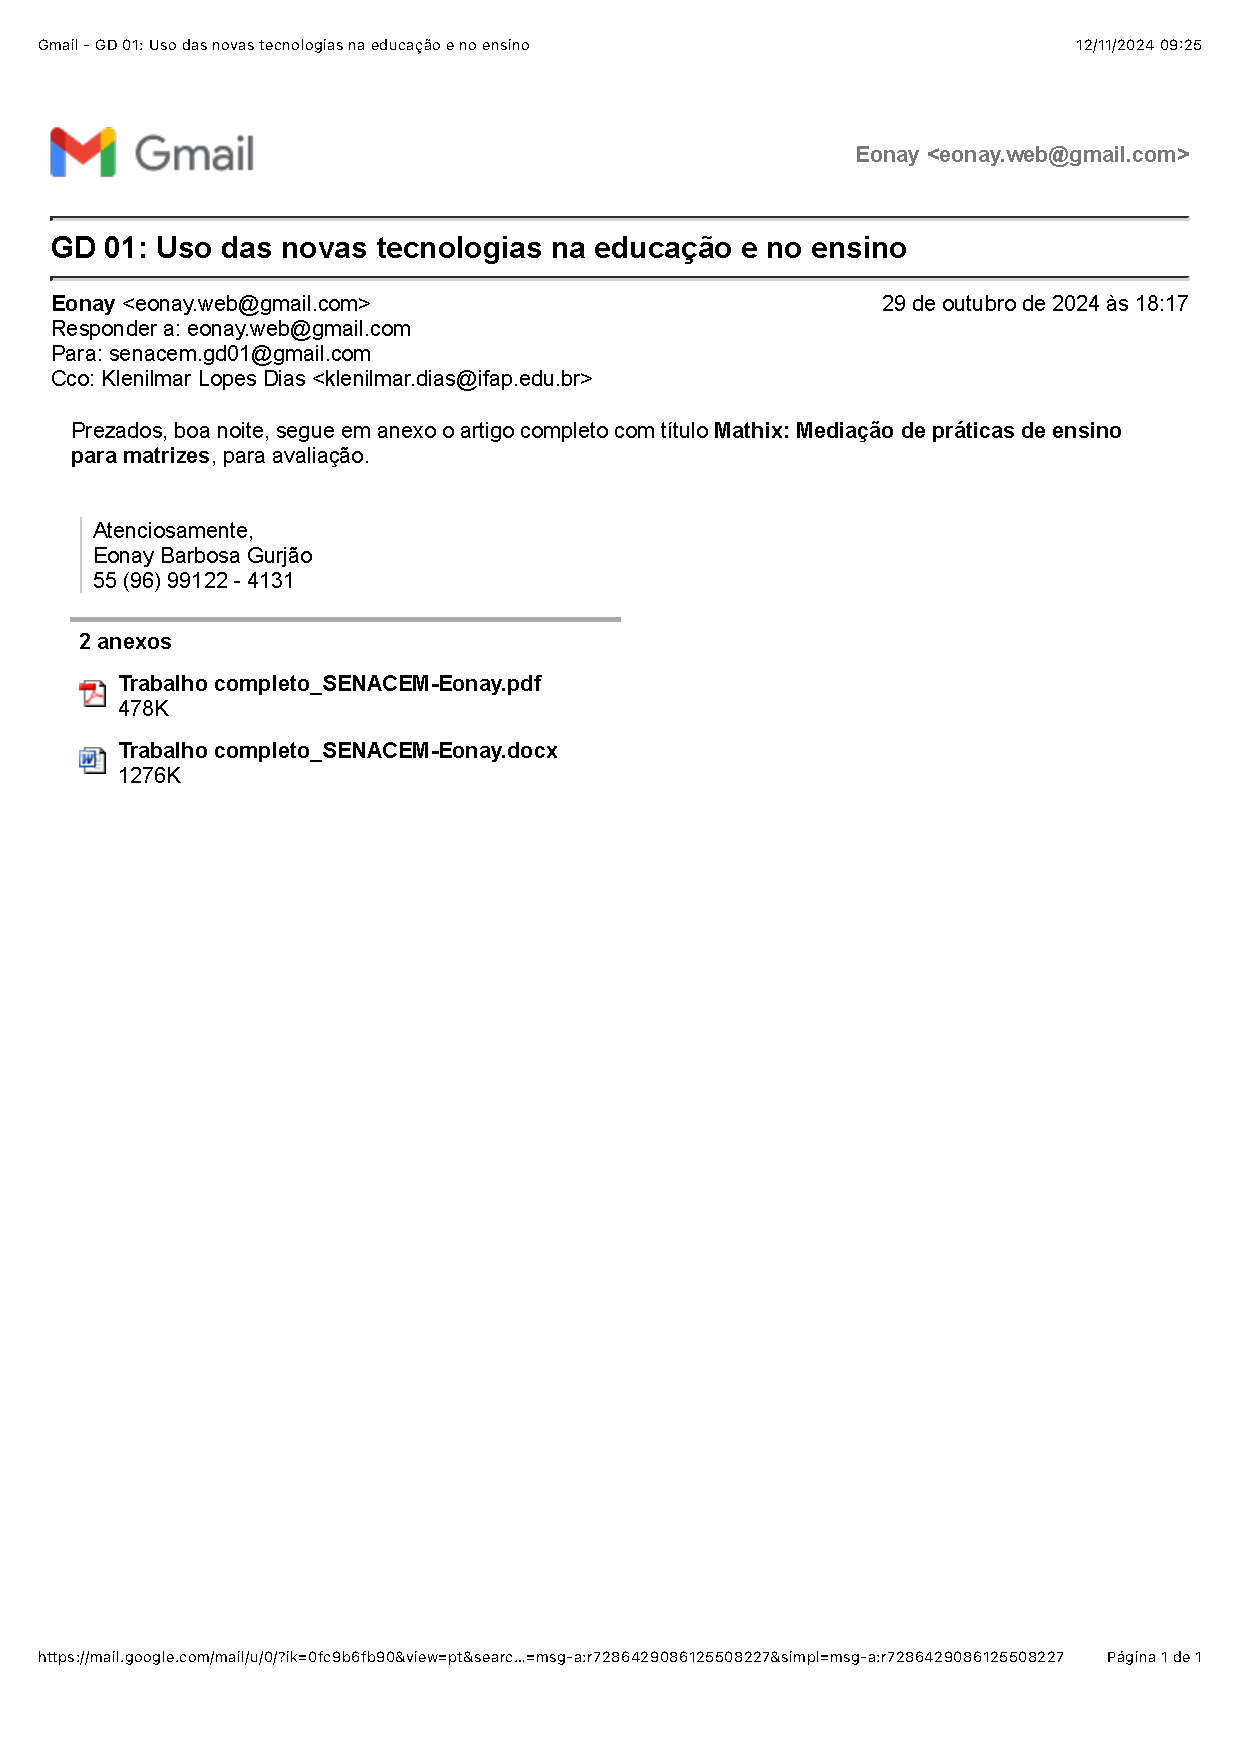
\includepdf[pages=-]{PosTextuais/submissao2.pdf}


% Anexo 05
\chapter{Relatório de Acesso aos Questionários }
\begin{center}
    Relatório de acesso aos questionário de avaliação emitidos via plataforma Survio.
\end{center}

\newpage
\begin{center}
    Relatório de acesso a avaliação do Produto Educacional.
    \newline
    \newline
    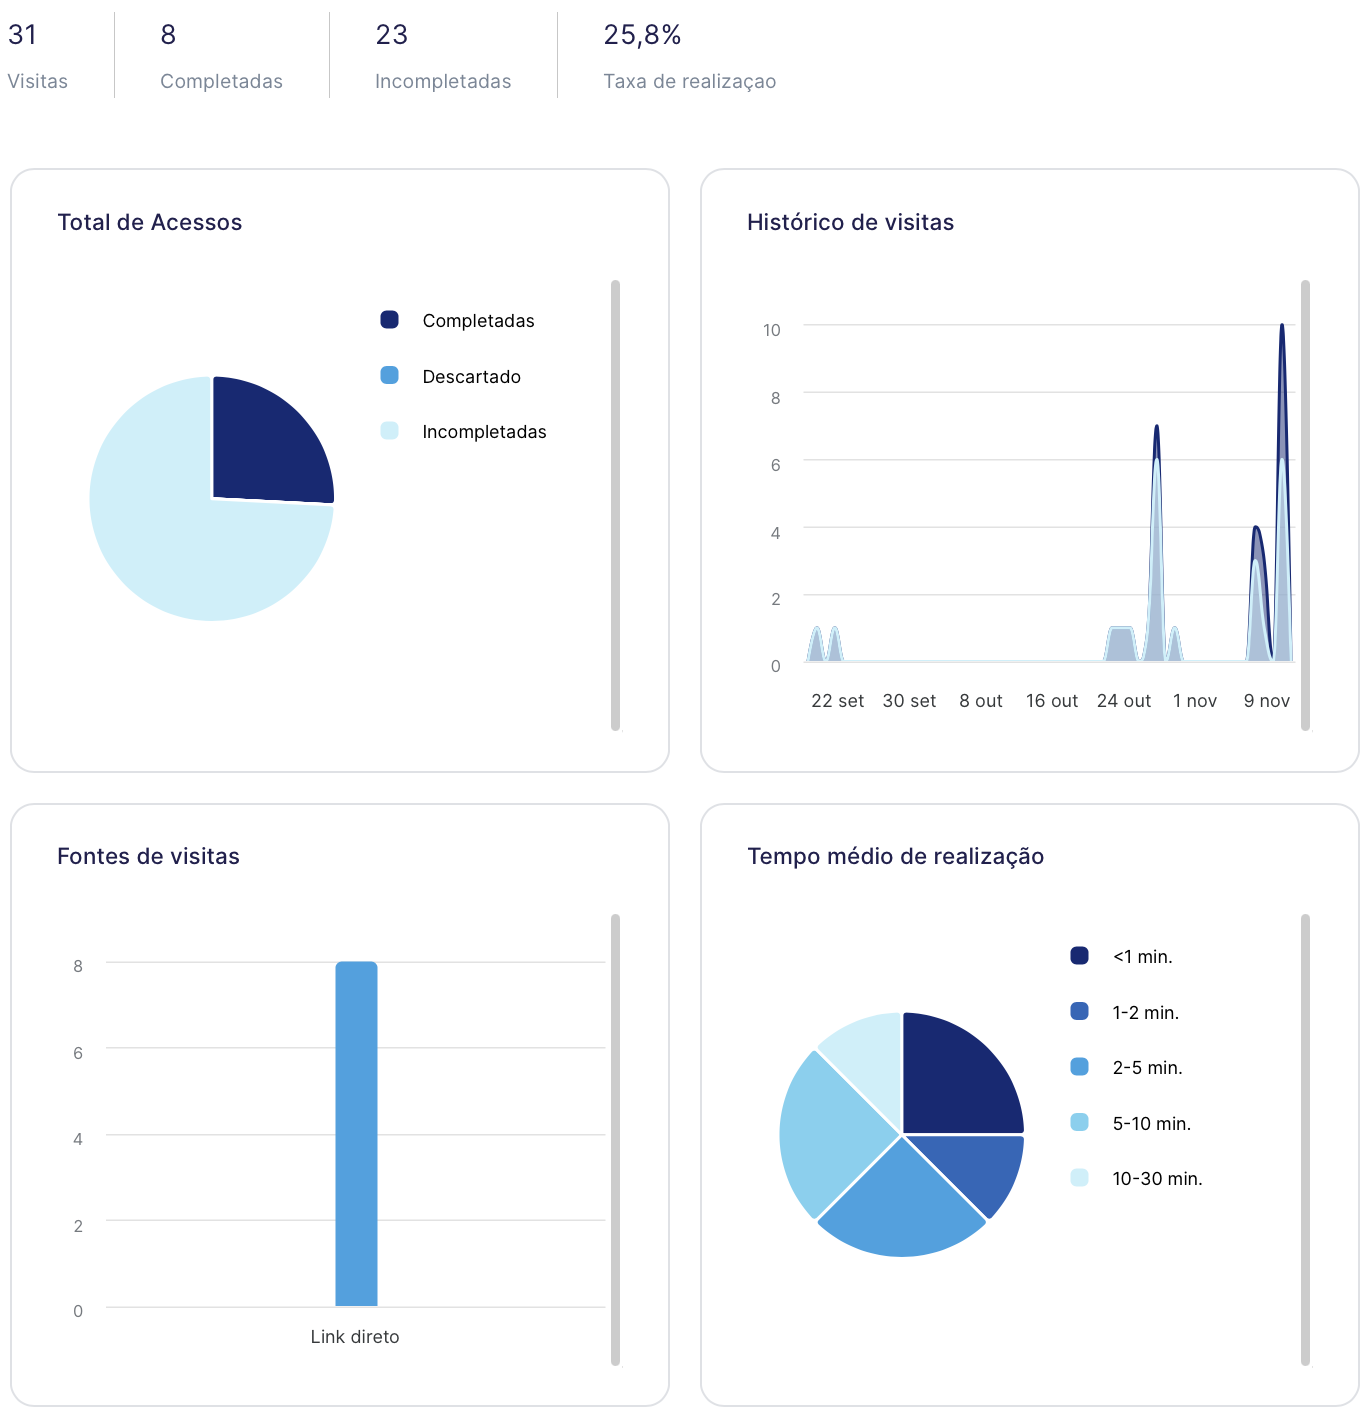
\includegraphics[width=\textwidth]{pos-textuais/anexo_pe.png}
\end{center}

\newpage
\begin{center}
    Relatório de acesso a avaliação de Interface de Usuário (UI) do Produto Educacional.
    \newline
    \newline
    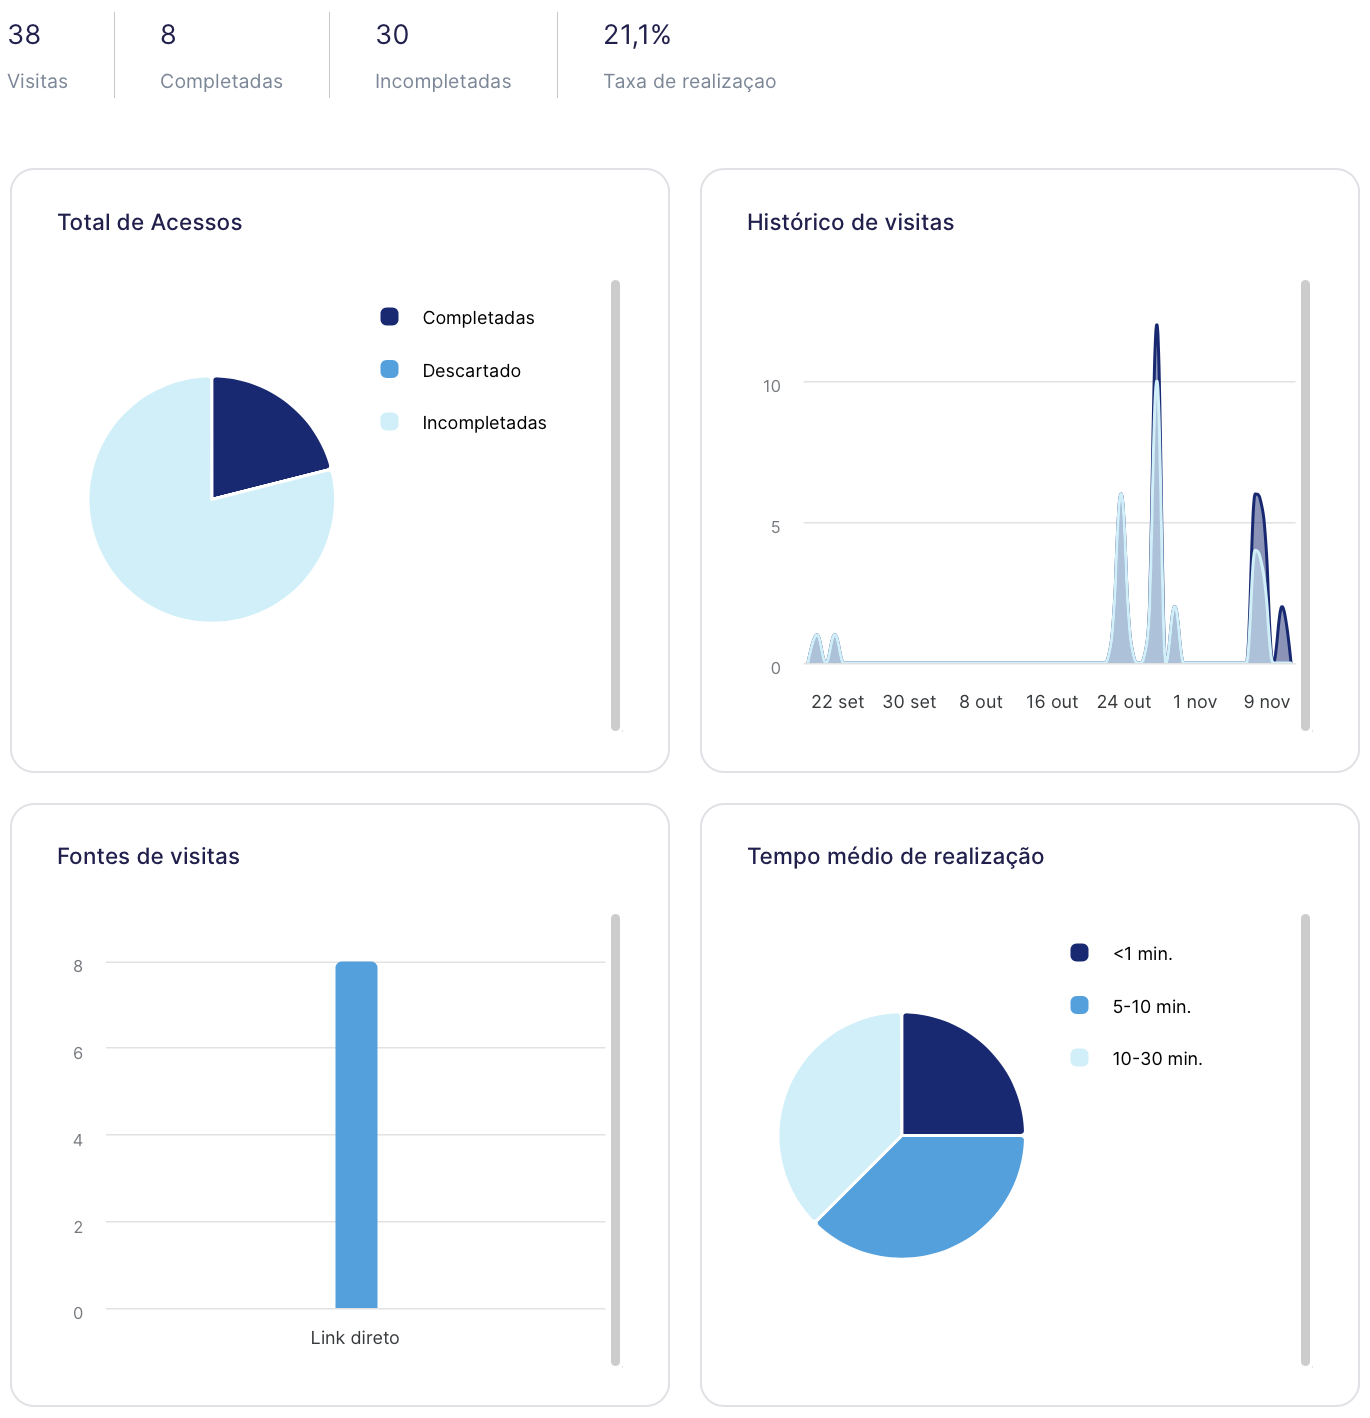
\includegraphics[width=\textwidth]{pos-textuais/anexo_ui.png}
\end{center}


\newpage
\begin{center}
    Relatório de acesso a avaliação de Experiência de Usuário (UX) do Produto Educacional.
    \newline
    \newline
    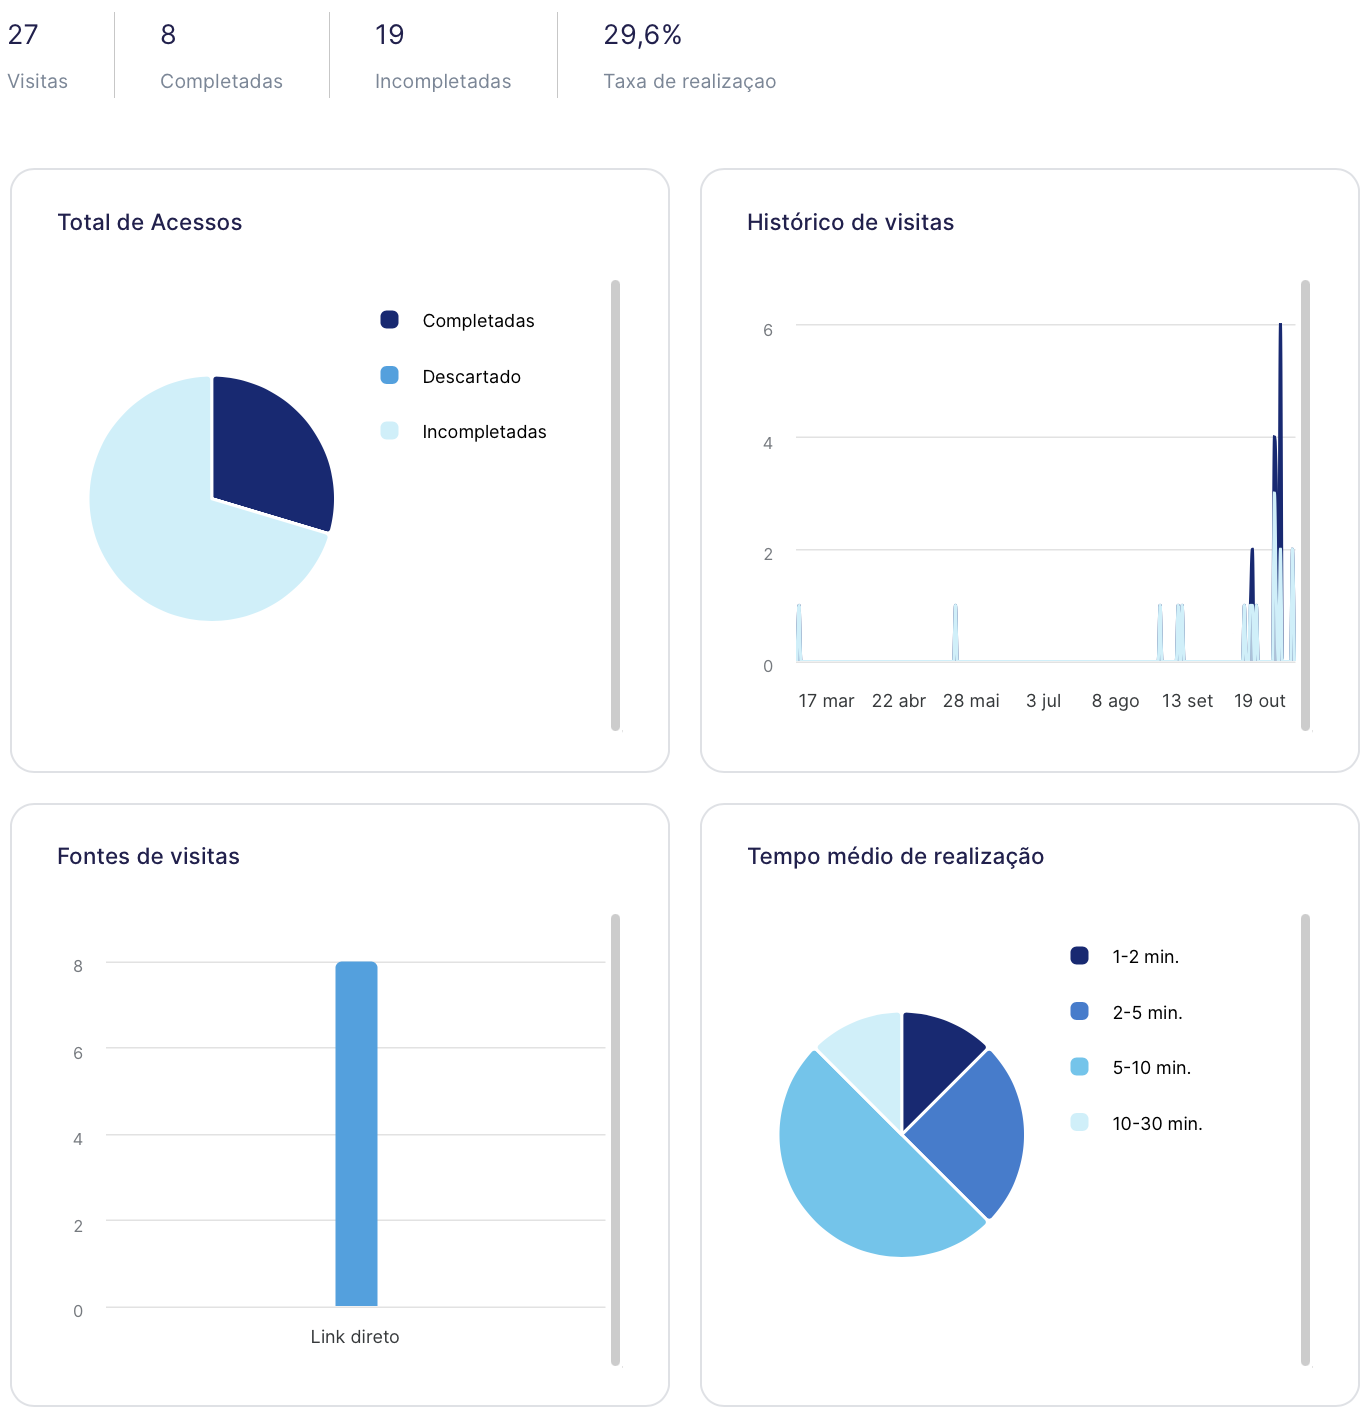
\includegraphics[width=\textwidth]{pos-textuais/anexo_ux.png}
\end{center}

\end{anexosenv}

%\phantompart  \printindex  % Indice Remissivo
% ----------------------------------------------------------
\end{document}  % fim do documento
